% Options for packages loaded elsewhere
\PassOptionsToPackage{unicode}{hyperref}
\PassOptionsToPackage{hyphens}{url}
%
\documentclass[
]{book}
\usepackage{lmodern}
\usepackage{amsmath}
\usepackage{ifxetex,ifluatex}
\ifnum 0\ifxetex 1\fi\ifluatex 1\fi=0 % if pdftex
  \usepackage[T1]{fontenc}
  \usepackage[utf8]{inputenc}
  \usepackage{textcomp} % provide euro and other symbols
  \usepackage{amssymb}
\else % if luatex or xetex
  \usepackage{unicode-math}
  \defaultfontfeatures{Scale=MatchLowercase}
  \defaultfontfeatures[\rmfamily]{Ligatures=TeX,Scale=1}
\fi
% Use upquote if available, for straight quotes in verbatim environments
\IfFileExists{upquote.sty}{\usepackage{upquote}}{}
\IfFileExists{microtype.sty}{% use microtype if available
  \usepackage[]{microtype}
  \UseMicrotypeSet[protrusion]{basicmath} % disable protrusion for tt fonts
}{}
\makeatletter
\@ifundefined{KOMAClassName}{% if non-KOMA class
  \IfFileExists{parskip.sty}{%
    \usepackage{parskip}
  }{% else
    \setlength{\parindent}{0pt}
    \setlength{\parskip}{6pt plus 2pt minus 1pt}}
}{% if KOMA class
  \KOMAoptions{parskip=half}}
\makeatother
\usepackage{xcolor}
\IfFileExists{xurl.sty}{\usepackage{xurl}}{} % add URL line breaks if available
\IfFileExists{bookmark.sty}{\usepackage{bookmark}}{\usepackage{hyperref}}
\hypersetup{
  pdftitle={Applied SNA with R},
  pdfauthor={George G. Vega Yon},
  hidelinks,
  pdfcreator={LaTeX via pandoc}}
\urlstyle{same} % disable monospaced font for URLs
\usepackage{color}
\usepackage{fancyvrb}
\newcommand{\VerbBar}{|}
\newcommand{\VERB}{\Verb[commandchars=\\\{\}]}
\DefineVerbatimEnvironment{Highlighting}{Verbatim}{commandchars=\\\{\}}
% Add ',fontsize=\small' for more characters per line
\usepackage{framed}
\definecolor{shadecolor}{RGB}{248,248,248}
\newenvironment{Shaded}{\begin{snugshade}}{\end{snugshade}}
\newcommand{\AlertTok}[1]{\textcolor[rgb]{0.94,0.16,0.16}{#1}}
\newcommand{\AnnotationTok}[1]{\textcolor[rgb]{0.56,0.35,0.01}{\textbf{\textit{#1}}}}
\newcommand{\AttributeTok}[1]{\textcolor[rgb]{0.77,0.63,0.00}{#1}}
\newcommand{\BaseNTok}[1]{\textcolor[rgb]{0.00,0.00,0.81}{#1}}
\newcommand{\BuiltInTok}[1]{#1}
\newcommand{\CharTok}[1]{\textcolor[rgb]{0.31,0.60,0.02}{#1}}
\newcommand{\CommentTok}[1]{\textcolor[rgb]{0.56,0.35,0.01}{\textit{#1}}}
\newcommand{\CommentVarTok}[1]{\textcolor[rgb]{0.56,0.35,0.01}{\textbf{\textit{#1}}}}
\newcommand{\ConstantTok}[1]{\textcolor[rgb]{0.00,0.00,0.00}{#1}}
\newcommand{\ControlFlowTok}[1]{\textcolor[rgb]{0.13,0.29,0.53}{\textbf{#1}}}
\newcommand{\DataTypeTok}[1]{\textcolor[rgb]{0.13,0.29,0.53}{#1}}
\newcommand{\DecValTok}[1]{\textcolor[rgb]{0.00,0.00,0.81}{#1}}
\newcommand{\DocumentationTok}[1]{\textcolor[rgb]{0.56,0.35,0.01}{\textbf{\textit{#1}}}}
\newcommand{\ErrorTok}[1]{\textcolor[rgb]{0.64,0.00,0.00}{\textbf{#1}}}
\newcommand{\ExtensionTok}[1]{#1}
\newcommand{\FloatTok}[1]{\textcolor[rgb]{0.00,0.00,0.81}{#1}}
\newcommand{\FunctionTok}[1]{\textcolor[rgb]{0.00,0.00,0.00}{#1}}
\newcommand{\ImportTok}[1]{#1}
\newcommand{\InformationTok}[1]{\textcolor[rgb]{0.56,0.35,0.01}{\textbf{\textit{#1}}}}
\newcommand{\KeywordTok}[1]{\textcolor[rgb]{0.13,0.29,0.53}{\textbf{#1}}}
\newcommand{\NormalTok}[1]{#1}
\newcommand{\OperatorTok}[1]{\textcolor[rgb]{0.81,0.36,0.00}{\textbf{#1}}}
\newcommand{\OtherTok}[1]{\textcolor[rgb]{0.56,0.35,0.01}{#1}}
\newcommand{\PreprocessorTok}[1]{\textcolor[rgb]{0.56,0.35,0.01}{\textit{#1}}}
\newcommand{\RegionMarkerTok}[1]{#1}
\newcommand{\SpecialCharTok}[1]{\textcolor[rgb]{0.00,0.00,0.00}{#1}}
\newcommand{\SpecialStringTok}[1]{\textcolor[rgb]{0.31,0.60,0.02}{#1}}
\newcommand{\StringTok}[1]{\textcolor[rgb]{0.31,0.60,0.02}{#1}}
\newcommand{\VariableTok}[1]{\textcolor[rgb]{0.00,0.00,0.00}{#1}}
\newcommand{\VerbatimStringTok}[1]{\textcolor[rgb]{0.31,0.60,0.02}{#1}}
\newcommand{\WarningTok}[1]{\textcolor[rgb]{0.56,0.35,0.01}{\textbf{\textit{#1}}}}
\usepackage{longtable,booktabs}
\usepackage{calc} % for calculating minipage widths
% Correct order of tables after \paragraph or \subparagraph
\usepackage{etoolbox}
\makeatletter
\patchcmd\longtable{\par}{\if@noskipsec\mbox{}\fi\par}{}{}
\makeatother
% Allow footnotes in longtable head/foot
\IfFileExists{footnotehyper.sty}{\usepackage{footnotehyper}}{\usepackage{footnote}}
\makesavenoteenv{longtable}
\usepackage{graphicx}
\makeatletter
\def\maxwidth{\ifdim\Gin@nat@width>\linewidth\linewidth\else\Gin@nat@width\fi}
\def\maxheight{\ifdim\Gin@nat@height>\textheight\textheight\else\Gin@nat@height\fi}
\makeatother
% Scale images if necessary, so that they will not overflow the page
% margins by default, and it is still possible to overwrite the defaults
% using explicit options in \includegraphics[width, height, ...]{}
\setkeys{Gin}{width=\maxwidth,height=\maxheight,keepaspectratio}
% Set default figure placement to htbp
\makeatletter
\def\fps@figure{htbp}
\makeatother
\setlength{\emergencystretch}{3em} % prevent overfull lines
\providecommand{\tightlist}{%
  \setlength{\itemsep}{0pt}\setlength{\parskip}{0pt}}
\setcounter{secnumdepth}{5}
\usepackage{booktabs}
\usepackage{hyperref}
  \hypersetup{allcolors=blue, colorlinks=true}

\usepackage{apacite}
\usepackage{setspace}
\onehalfspacing

\usepackage{arev}
\usepackage[T1]{fontenc}

\usepackage[margin=1in]{geometry}

\ifluatex
  \usepackage{selnolig}  % disable illegal ligatures
\fi
\newlength{\cslhangindent}
\setlength{\cslhangindent}{1.5em}
\newlength{\csllabelwidth}
\setlength{\csllabelwidth}{3em}
\newenvironment{CSLReferences}[2] % #1 hanging-ident, #2 entry spacing
 {% don't indent paragraphs
  \setlength{\parindent}{0pt}
  % turn on hanging indent if param 1 is 1
  \ifodd #1 \everypar{\setlength{\hangindent}{\cslhangindent}}\ignorespaces\fi
  % set entry spacing
  \ifnum #2 > 0
  \setlength{\parskip}{#2\baselineskip}
  \fi
 }%
 {}
\usepackage{calc}
\newcommand{\CSLBlock}[1]{#1\hfill\break}
\newcommand{\CSLLeftMargin}[1]{\parbox[t]{\csllabelwidth}{#1}}
\newcommand{\CSLRightInline}[1]{\parbox[t]{\linewidth - \csllabelwidth}{#1}\break}
\newcommand{\CSLIndent}[1]{\hspace{\cslhangindent}#1}

\title{Applied SNA with R}
\author{George G. Vega Yon}
\date{2021-04-27}

\begin{document}
\maketitle

{
\setcounter{tocdepth}{1}
\tableofcontents
}
\hypertarget{about-this-book}{%
\chapter{About this book}\label{about-this-book}}

\renewcommand{\Pr}[1]{\mbox{Pr}\left(#1\right)}
\renewcommand{\exp}[1]{\mbox{exp}\left\{#1\right\}}

This book will be build as part of a workshop on Applied Social Network Analysis with R. Its contents will be populated as the sessions take place, and for now there is particular program that we will follow, instead, we have the following workflow:

\begin{enumerate}
\def\labelenumi{\arabic{enumi}.}
\item
  Participants will share their data and what they need to do with it.
\item
  Based on their data, I'll be preparing the sessions trying to show attendees how would I approach the problem, and at the same time, teach by example about the R language.
\item
  Materials will be published on this website and, hopefully, video recordings of the sessions.
\end{enumerate}

At least in the first version, the book will be organized by session, this is, one chapter per session.

All the book materials can be downloaded from \url{https://github.com/gvegayon/appliedsnar}

In general, we will besides of R itself, we will be using R studio and the following R packages: dplyr for data management, stringr for data cleaning, and of course igraph, netdiffuseR (a bit of a bias here), and statnet for our neat network analysis.\footnote{Some of you may be wondering ``what about ggplot2 and friends? What about \href{https://www.tidyverse.org/}{\texttt{tidyverse}},'' well, my short answer is I jumped into R before all of that was that popular. When I started plots were all about \href{https://CRAN.R-project.org/package=lattice}{\texttt{lattice}}, and after a couple of years on that, about base R graphics. What I'm saying is that so far I have not find a compelling reason to leave my ``old-practices'' and embrace all the \texttt{tidyverse} movement (religion?).}

\hypertarget{introduction}{%
\chapter{Introduction}\label{introduction}}

For this book we need the following

\protect\hyperlink{ref-R}{R Core Team} (\protect\hyperlink{ref-R}{2017b})

\begin{enumerate}
\def\labelenumi{\arabic{enumi}.}
\item
  Install R from CRAN: \url{https://www.r-project.org/}
\item
  (optional) Install Rstudio: \url{https://rstudio.org}
\end{enumerate}

While I find RStudio extreamly useful, it is not necesary to use it with R.

\hypertarget{r-basics}{%
\chapter{R Basics}\label{r-basics}}

\hypertarget{what-is-r}{%
\section{What is R}\label{what-is-r}}

A good reference book for both new and advanced user is \href{https://nostarch.com/artofr.htm}{``The Art of R programming''} (\protect\hyperlink{ref-Matloff2011}{Matloff 2011})\footnote{\href{http://heather.cs.ucdavis.edu/~matloff/145/PLN/RMaterials/NSPpart.pdf}{Here} a free pdf version distributed by the author.}

\hypertarget{how-to-install-packages}{%
\section{How to install packages}\label{how-to-install-packages}}

Nowadays there are two ways of installing R packages (that I'm aware of), either using \texttt{install.packages}, which is a function shipped with R, or use the devtools R package to install a package from some remote repository other than CRAN, here is a couple of examples:

\begin{Shaded}
\begin{Highlighting}[]
\CommentTok{\# This will install the igraph package from CRAN}
\SpecialCharTok{\textgreater{}} \FunctionTok{install.packages}\NormalTok{(}\StringTok{"netdiffuseR"}\NormalTok{)}

\CommentTok{\# This will install the bleeding{-}edge version from the project\textquotesingle{}s github repo!}
\SpecialCharTok{\textgreater{}}\NormalTok{ devtools}\SpecialCharTok{::}\FunctionTok{install\_github}\NormalTok{(}\StringTok{"USCCANA/netdiffuseR"}\NormalTok{)}
\end{Highlighting}
\end{Shaded}

The first one, using \texttt{install.packages}, installs the CRAN version of \texttt{netdiffuseR}, whereas the second installs whatever version is plublished on \url{https://github.com/USCCANA/netdiffuseR}, which is usually called the development version.

In some cases users may want/need to install packages from command line as some packages need extra configuration to be installed. But we won't need to look at it now.

\hypertarget{network-nomination-data}{%
\chapter{Network Nomination Data}\label{network-nomination-data}}

The data can be downloaded from \href{https://cdn.rawgit.com/gvegayon/appliedsnar/fdc0d26f/03-sns.dta}{here}.

The codebook for the data provided here is in \protect\hyperlink{sns-data}{the appendix}.

This chapter's goals are:

\begin{enumerate}
\def\labelenumi{\arabic{enumi}.}
\item
  Read the data into R,
\item
  Create a network with it,
\item
  Compute descriptive statistics
\item
  Visualize the network
\end{enumerate}

\hypertarget{data-preprocessing}{%
\section{Data preprocessing}\label{data-preprocessing}}

\hypertarget{reading-the-data-into-r}{%
\subsection{Reading the data into R}\label{reading-the-data-into-r}}

R has several ways of reading data in. You data can be Raw plain files like CSV, tab delimited or specified by column width, for which you can use the \href{https://cran.r-project.org/package=readr}{\texttt{readr}} package (\protect\hyperlink{ref-R-readr}{Wickham, Hester, and Francois 2017}); or it can be binary files like dta (Stata), Octave, SPSS, for which \href{https://cran.r-project.org/package=readr}{\texttt{foreign}} (\protect\hyperlink{ref-R-foreign}{R Core Team 2017a}) can be used; or it could be excel files in which case you should be using \href{https://cran.r-project.org/package=readxl}{\texttt{readxl}} (\protect\hyperlink{ref-R-readxl}{Wickham and Bryan 2017}). In our case, the data for this session is in Stata format:

\begin{Shaded}
\begin{Highlighting}[]
\FunctionTok{library}\NormalTok{(foreign)}

\CommentTok{\# Reading the data}
\NormalTok{dat }\OtherTok{\textless{}{-}}\NormalTok{ foreign}\SpecialCharTok{::}\FunctionTok{read.dta}\NormalTok{(}\StringTok{"03{-}sns.dta"}\NormalTok{)}

\CommentTok{\# Taking a look at the data\textquotesingle{}s first 5 columns and 5 rows}
\NormalTok{dat[}\DecValTok{1}\SpecialCharTok{:}\DecValTok{5}\NormalTok{, }\DecValTok{1}\SpecialCharTok{:}\DecValTok{10}\NormalTok{]}
\end{Highlighting}
\end{Shaded}

\begin{verbatim}
##   photoid school hispanic female1 female2 female3 female4 grades1 grades2
## 1       1    111        1      NA      NA       0       0      NA      NA
## 2       2    111        1       0      NA      NA       0     3.0      NA
## 3       7    111        0       1       1       1       1     5.0     4.5
## 4      13    111        1       1       1       1       1     2.5     2.5
## 5      14    111        1       1       1       1      NA     3.0     3.5
##   grades3
## 1     3.5
## 2      NA
## 3     4.0
## 4     2.5
## 5     3.5
\end{verbatim}

\hypertarget{creating-a-unique-id-for-each-participant}{%
\subsection{Creating a unique id for each participant}\label{creating-a-unique-id-for-each-participant}}

Now suppose that we want to create a unique id using the school and photo id. In this case, since both variables are numeric, a good way of doing it is to encode the id such that, for example, the last three \texttt{x} numbers are the photoid and the first ones are the school id. To do this we need to take into account the range of the variables. Here, \texttt{photoid} has the following range:

\begin{Shaded}
\begin{Highlighting}[]
\NormalTok{(photo\_id\_ran }\OtherTok{\textless{}{-}} \FunctionTok{range}\NormalTok{(dat}\SpecialCharTok{$}\NormalTok{photoid))}
\end{Highlighting}
\end{Shaded}

\begin{verbatim}
## [1]    1 2074
\end{verbatim}

As the variable spans up to 2074, we need to set the last 4 units of the variable to store the \texttt{photoid}. We will use \texttt{dplyr} (\protect\hyperlink{ref-R-dplyr}{Wickham et al. 2017}) and \texttt{magrittr} (\protect\hyperlink{ref-R-magrittr}{Bache and Wickham 2014}){]} (the pipe operator, \texttt{\%\textgreater{}\%}) to create this variable, and we will call it\ldots{} \texttt{id} (mind blowing, right?):

\begin{Shaded}
\begin{Highlighting}[]
\FunctionTok{library}\NormalTok{(dplyr)}
\end{Highlighting}
\end{Shaded}

\begin{verbatim}
## 
## Attaching package: 'dplyr'
\end{verbatim}

\begin{verbatim}
## The following objects are masked from 'package:stats':
## 
##     filter, lag
\end{verbatim}

\begin{verbatim}
## The following objects are masked from 'package:base':
## 
##     intersect, setdiff, setequal, union
\end{verbatim}

\begin{Shaded}
\begin{Highlighting}[]
\FunctionTok{library}\NormalTok{(magrittr)}

\NormalTok{(dat }\SpecialCharTok{\%\textless{}\textgreater{}\%} \FunctionTok{mutate}\NormalTok{(}\AttributeTok{id =}\NormalTok{ school}\SpecialCharTok{*}\DecValTok{10000} \SpecialCharTok{+}\NormalTok{ photoid)) }\SpecialCharTok{\%\textgreater{}\%}
\NormalTok{  head }\SpecialCharTok{\%\textgreater{}\%}
  \FunctionTok{select}\NormalTok{(school, photoid, id)}
\end{Highlighting}
\end{Shaded}

\begin{verbatim}
##   school photoid      id
## 1    111       1 1110001
## 2    111       2 1110002
## 3    111       7 1110007
## 4    111      13 1110013
## 5    111      14 1110014
## 6    111      15 1110015
\end{verbatim}

Wow, what happend in the last three lines of code! What is that \texttt{\%\textgreater{}\%}? Well, that's the \href{http://r4ds.had.co.nz/pipes.html}{piping operator}, and it is a very nice way of writing nested function calls. In this case, instead of having write something like

\begin{Shaded}
\begin{Highlighting}[]
\NormalTok{dat\_filtered}\SpecialCharTok{$}\NormalTok{id }\OtherTok{\textless{}{-}}\NormalTok{ dat\_filtered}\SpecialCharTok{$}\NormalTok{school}\SpecialCharTok{*}\DecValTok{10000} \SpecialCharTok{+}\NormalTok{ dat\_filtered}\SpecialCharTok{$}\NormalTok{photoid}
\FunctionTok{subset}\NormalTok{(}\FunctionTok{head}\NormalTok{(dat\_filtered), }\AttributeTok{select =} \FunctionTok{c}\NormalTok{(school, photoid, id))}
\end{Highlighting}
\end{Shaded}

\hypertarget{creating-a-network}{%
\section{Creating a network}\label{creating-a-network}}

\begin{itemize}
\item
  We want to build a social network. For that, we either use an adjacency matrix or an edgelist.
\item
  Each individual of the SNS data nomitated 19 friends from school. We will use those nominations to create the social network.
\item
  In this case, we will create the network by coercing the dataset into an edgelist.
\end{itemize}

\hypertarget{from-survey-to-edgelist}{%
\subsection{From survey to edgelist}\label{from-survey-to-edgelist}}

Let's start by loading a couple of handy R packages for this task, \texttt{tidyr} (\protect\hyperlink{ref-R-tidyr}{Wickham and Henry 2017}), which we will use to reshape the data, and \texttt{stringr} (\protect\hyperlink{ref-R-stringr}{Wickham 2017}), which we will use to process strings using \emph{regular expressions}\footnote{Please refer to the help file \texttt{?\textquotesingle{}regular\ expression\textquotesingle{}} in R. The R package \texttt{rex} (\protect\hyperlink{ref-R-rex}{Ushey, Hester, and Krzyzanowski 2017}) is a very nice companion for writing regular expressions. There's also a neat (but experimental) RStudio addin that can be very helpful for understanding how regular expressions work, the \href{https://github.com/gadenbuie/regexplain}{regexplain} addin.}.

\begin{Shaded}
\begin{Highlighting}[]
\FunctionTok{library}\NormalTok{(tidyr)}
\FunctionTok{library}\NormalTok{(stringr)}
\end{Highlighting}
\end{Shaded}

Optionally, we can use the \texttt{tibble} type of object which is an alternative to the actual \texttt{data.frame}. This object is claimed to provide \emph{more efficient methods for matrices and data frames}.

\begin{Shaded}
\begin{Highlighting}[]
\NormalTok{dat }\OtherTok{\textless{}{-}} \FunctionTok{as\_tibble}\NormalTok{(dat)}
\end{Highlighting}
\end{Shaded}

What I like from tibbles is that when you print them on the console these actually look nice:

\begin{Shaded}
\begin{Highlighting}[]
\NormalTok{dat}
\end{Highlighting}
\end{Shaded}

\begin{verbatim}
## # A tibble: 2,164 x 100
##    photoid school hispanic female1 female2 female3 female4 grades1 grades2
##      <int>  <int>    <dbl>   <int>   <int>   <int>   <int>   <dbl>   <dbl>
##  1       1    111        1      NA      NA       0       0    NA      NA  
##  2       2    111        1       0      NA      NA       0     3      NA  
##  3       7    111        0       1       1       1       1     5       4.5
##  4      13    111        1       1       1       1       1     2.5     2.5
##  5      14    111        1       1       1       1      NA     3       3.5
##  6      15    111        1       0       0       0       0     2.5     2.5
##  7      20    111        1       1       1       1       1     2.5     2.5
##  8      22    111        1      NA      NA       0       0    NA      NA  
##  9      25    111        0       1       1      NA       1     4.5     3.5
## 10      27    111        1       0      NA       0       0     3.5    NA  
## # ... with 2,154 more rows, and 91 more variables: grades3 <dbl>,
## #   grades4 <dbl>, eversmk1 <int>, eversmk2 <int>, eversmk3 <int>,
## #   eversmk4 <int>, everdrk1 <int>, everdrk2 <int>, everdrk3 <int>,
## #   everdrk4 <int>, home1 <int>, home2 <int>, home3 <int>, home4 <int>,
## #   sch_friend11 <int>, sch_friend12 <int>, sch_friend13 <int>,
## #   sch_friend14 <int>, sch_friend15 <int>, sch_friend16 <int>,
## #   sch_friend17 <int>, sch_friend18 <int>, sch_friend19 <int>,
## #   sch_friend110 <int>, sch_friend111 <int>, sch_friend112 <int>,
## #   sch_friend113 <int>, sch_friend114 <int>, sch_friend115 <int>,
## #   sch_friend116 <int>, sch_friend117 <int>, sch_friend118 <int>,
## #   sch_friend119 <int>, sch_friend21 <int>, sch_friend22 <int>,
## #   sch_friend23 <int>, sch_friend24 <int>, sch_friend25 <int>,
## #   sch_friend26 <int>, sch_friend27 <int>, sch_friend28 <int>,
## #   sch_friend29 <int>, sch_friend210 <int>, sch_friend211 <int>,
## #   sch_friend212 <int>, sch_friend213 <int>, sch_friend214 <int>,
## #   sch_friend215 <int>, sch_friend216 <int>, sch_friend217 <int>,
## #   sch_friend218 <int>, sch_friend219 <int>, sch_friend31 <int>,
## #   sch_friend32 <int>, sch_friend33 <int>, sch_friend34 <int>,
## #   sch_friend35 <int>, sch_friend36 <int>, sch_friend37 <int>,
## #   sch_friend38 <int>, sch_friend39 <int>, sch_friend310 <int>,
## #   sch_friend311 <int>, sch_friend312 <int>, sch_friend313 <int>,
## #   sch_friend314 <int>, sch_friend315 <int>, sch_friend316 <int>,
## #   sch_friend317 <int>, sch_friend318 <int>, sch_friend319 <int>,
## #   sch_friend41 <int>, sch_friend42 <int>, sch_friend43 <int>,
## #   sch_friend44 <int>, sch_friend45 <int>, sch_friend46 <int>,
## #   sch_friend47 <int>, sch_friend48 <int>, sch_friend49 <int>,
## #   sch_friend410 <int>, sch_friend411 <int>, sch_friend412 <int>,
## #   sch_friend413 <int>, sch_friend414 <int>, sch_friend415 <int>,
## #   sch_friend416 <int>, sch_friend417 <int>, sch_friend418 <int>,
## #   sch_friend419 <int>, id <dbl>
\end{verbatim}

\begin{Shaded}
\begin{Highlighting}[]
\CommentTok{\# Maybe too much piping... but its cool!}
\NormalTok{net }\OtherTok{\textless{}{-}}\NormalTok{ dat }\SpecialCharTok{\%\textgreater{}\%} 
  \FunctionTok{select}\NormalTok{(id, school, }\FunctionTok{starts\_with}\NormalTok{(}\StringTok{"sch\_friend"}\NormalTok{)) }\SpecialCharTok{\%\textgreater{}\%}
  \FunctionTok{gather}\NormalTok{(}\AttributeTok{key =} \StringTok{"varname"}\NormalTok{, }\AttributeTok{value =} \StringTok{"content"}\NormalTok{, }\SpecialCharTok{{-}}\NormalTok{id, }\SpecialCharTok{{-}}\NormalTok{school) }\SpecialCharTok{\%\textgreater{}\%}
  \FunctionTok{filter}\NormalTok{(}\SpecialCharTok{!}\FunctionTok{is.na}\NormalTok{(content)) }\SpecialCharTok{\%\textgreater{}\%}
  \FunctionTok{mutate}\NormalTok{(}
    \AttributeTok{friendid =}\NormalTok{ school}\SpecialCharTok{*}\DecValTok{10000} \SpecialCharTok{+}\NormalTok{ content,}
    \AttributeTok{year     =} \FunctionTok{as.integer}\NormalTok{(}\FunctionTok{str\_extract}\NormalTok{(varname, }\StringTok{"(?\textless{}=[a{-}z])[0{-}9]"}\NormalTok{)),}
    \AttributeTok{nnom     =} \FunctionTok{as.integer}\NormalTok{(}\FunctionTok{str\_extract}\NormalTok{(varname, }\StringTok{"(?\textless{}=[a{-}z][0{-}9])[0{-}9]+"}\NormalTok{))}
\NormalTok{  )}
\end{Highlighting}
\end{Shaded}

Let's take a look at this step by step:

\begin{enumerate}
\def\labelenumi{\arabic{enumi}.}
\item
  First, we subset the data: We want to keep \texttt{id,\ school,\ sch\_friend*}. For the later we use the function \texttt{starts\_with} (from the \texttt{tidyselect} package). This allows us to select all variables that starts with the word ``\texttt{sch\_friend},'' which means that \texttt{sch\_friend11,\ sch\_friend12,\ ...} will all be selected.

\begin{Shaded}
\begin{Highlighting}[]
\NormalTok{dat }\SpecialCharTok{\%\textgreater{}\%} 
  \FunctionTok{select}\NormalTok{(id, school, }\FunctionTok{starts\_with}\NormalTok{(}\StringTok{"sch\_friend"}\NormalTok{))}
\end{Highlighting}
\end{Shaded}

\begin{verbatim}
## # A tibble: 2,164 x 78
##        id school sch_friend11 sch_friend12 sch_friend13 sch_friend14
##     <dbl>  <int>        <int>        <int>        <int>        <int>
##  1 1.11e6    111           NA           NA           NA           NA
##  2 1.11e6    111          424          423          426          289
##  3 1.11e6    111          629          505           NA           NA
##  4 1.11e6    111          232          569           NA           NA
##  5 1.11e6    111          582          134           41          592
##  6 1.11e6    111           26          488           81          138
##  7 1.11e6    111          528           NA          492          395
##  8 1.11e6    111           NA           NA           NA           NA
##  9 1.11e6    111          135          185          553           84
## 10 1.11e6    111          346          168          559            5
## # ... with 2,154 more rows, and 72 more variables: sch_friend15 <int>,
## #   sch_friend16 <int>, sch_friend17 <int>, sch_friend18 <int>,
## #   sch_friend19 <int>, sch_friend110 <int>, sch_friend111 <int>,
## #   sch_friend112 <int>, sch_friend113 <int>, sch_friend114 <int>,
## #   sch_friend115 <int>, sch_friend116 <int>, sch_friend117 <int>,
## #   sch_friend118 <int>, sch_friend119 <int>, sch_friend21 <int>,
## #   sch_friend22 <int>, sch_friend23 <int>, sch_friend24 <int>,
## #   sch_friend25 <int>, sch_friend26 <int>, sch_friend27 <int>,
## #   sch_friend28 <int>, sch_friend29 <int>, sch_friend210 <int>,
## #   sch_friend211 <int>, sch_friend212 <int>, sch_friend213 <int>,
## #   sch_friend214 <int>, sch_friend215 <int>, sch_friend216 <int>,
## #   sch_friend217 <int>, sch_friend218 <int>, sch_friend219 <int>,
## #   sch_friend31 <int>, sch_friend32 <int>, sch_friend33 <int>,
## #   sch_friend34 <int>, sch_friend35 <int>, sch_friend36 <int>,
## #   sch_friend37 <int>, sch_friend38 <int>, sch_friend39 <int>,
## #   sch_friend310 <int>, sch_friend311 <int>, sch_friend312 <int>,
## #   sch_friend313 <int>, sch_friend314 <int>, sch_friend315 <int>,
## #   sch_friend316 <int>, sch_friend317 <int>, sch_friend318 <int>,
## #   sch_friend319 <int>, sch_friend41 <int>, sch_friend42 <int>,
## #   sch_friend43 <int>, sch_friend44 <int>, sch_friend45 <int>,
## #   sch_friend46 <int>, sch_friend47 <int>, sch_friend48 <int>,
## #   sch_friend49 <int>, sch_friend410 <int>, sch_friend411 <int>,
## #   sch_friend412 <int>, sch_friend413 <int>, sch_friend414 <int>,
## #   sch_friend415 <int>, sch_friend416 <int>, sch_friend417 <int>,
## #   sch_friend418 <int>, sch_friend419 <int>
\end{verbatim}
\item
  Then, we reshape it to \emph{long} format: By transposing all the \texttt{sch\_friend*} to long. We do this by means of the function \texttt{gather} (from the \texttt{tidyr} package). This is an alternative to the \texttt{reshape} function, and I personally find it easier to use. Let's see how it works:

\begin{Shaded}
\begin{Highlighting}[]
\NormalTok{dat }\SpecialCharTok{\%\textgreater{}\%} 
  \FunctionTok{select}\NormalTok{(id, school, }\FunctionTok{starts\_with}\NormalTok{(}\StringTok{"sch\_friend"}\NormalTok{)) }\SpecialCharTok{\%\textgreater{}\%}
  \FunctionTok{gather}\NormalTok{(}\AttributeTok{key =} \StringTok{"varname"}\NormalTok{, }\AttributeTok{value =} \StringTok{"content"}\NormalTok{, }\SpecialCharTok{{-}}\NormalTok{id, }\SpecialCharTok{{-}}\NormalTok{school)}
\end{Highlighting}
\end{Shaded}

\begin{verbatim}
## # A tibble: 164,464 x 4
##         id school varname      content
##      <dbl>  <int> <chr>          <int>
##  1 1110001    111 sch_friend11      NA
##  2 1110002    111 sch_friend11     424
##  3 1110007    111 sch_friend11     629
##  4 1110013    111 sch_friend11     232
##  5 1110014    111 sch_friend11     582
##  6 1110015    111 sch_friend11      26
##  7 1110020    111 sch_friend11     528
##  8 1110022    111 sch_friend11      NA
##  9 1110025    111 sch_friend11     135
## 10 1110027    111 sch_friend11     346
## # ... with 164,454 more rows
\end{verbatim}

  In this case the \texttt{key} parameter sets the name of the variable that will contain the name of the variable that was reshaped, while \texttt{value} is the name of the variable that will hold the content of the data (that's why I named those like that). The \texttt{-id,\ -school} bit tells the function to ``drop'' those variables before reshaping, in other words, ``reshape everything but \texttt{id} and \texttt{school}.''

  Also, notice that we passed from 2164 rows to 19 (nominations) * 2164 (subjects) * 4 (waves) = 164464 rows, as expected.
\item
  As the nomination data can be empty for some cells, we need to take care of those cases, the \texttt{NA}s, so we filter the data:

\begin{Shaded}
\begin{Highlighting}[]
\NormalTok{dat }\SpecialCharTok{\%\textgreater{}\%} 
  \FunctionTok{select}\NormalTok{(id, school, }\FunctionTok{starts\_with}\NormalTok{(}\StringTok{"sch\_friend"}\NormalTok{)) }\SpecialCharTok{\%\textgreater{}\%}
  \FunctionTok{gather}\NormalTok{(}\AttributeTok{key =} \StringTok{"varname"}\NormalTok{, }\AttributeTok{value =} \StringTok{"content"}\NormalTok{, }\SpecialCharTok{{-}}\NormalTok{id, }\SpecialCharTok{{-}}\NormalTok{school) }\SpecialCharTok{\%\textgreater{}\%}
  \FunctionTok{filter}\NormalTok{(}\SpecialCharTok{!}\FunctionTok{is.na}\NormalTok{(content))}
\end{Highlighting}
\end{Shaded}

\begin{verbatim}
## # A tibble: 39,561 x 4
##         id school varname      content
##      <dbl>  <int> <chr>          <int>
##  1 1110002    111 sch_friend11     424
##  2 1110007    111 sch_friend11     629
##  3 1110013    111 sch_friend11     232
##  4 1110014    111 sch_friend11     582
##  5 1110015    111 sch_friend11      26
##  6 1110020    111 sch_friend11     528
##  7 1110025    111 sch_friend11     135
##  8 1110027    111 sch_friend11     346
##  9 1110029    111 sch_friend11     369
## 10 1110030    111 sch_friend11     462
## # ... with 39,551 more rows
\end{verbatim}
\item
  And finally, we create three new variables from this dataset: \texttt{friendid}, \texttt{year}, and \texttt{nom\_num} (nomination number). All this using regular expressions:

\begin{Shaded}
\begin{Highlighting}[]
\NormalTok{dat }\SpecialCharTok{\%\textgreater{}\%} 
  \FunctionTok{select}\NormalTok{(id, school, }\FunctionTok{starts\_with}\NormalTok{(}\StringTok{"sch\_friend"}\NormalTok{)) }\SpecialCharTok{\%\textgreater{}\%}
  \FunctionTok{gather}\NormalTok{(}\AttributeTok{key =} \StringTok{"varname"}\NormalTok{, }\AttributeTok{value =} \StringTok{"content"}\NormalTok{, }\SpecialCharTok{{-}}\NormalTok{id, }\SpecialCharTok{{-}}\NormalTok{school) }\SpecialCharTok{\%\textgreater{}\%}
  \FunctionTok{filter}\NormalTok{(}\SpecialCharTok{!}\FunctionTok{is.na}\NormalTok{(content)) }\SpecialCharTok{\%\textgreater{}\%}
  \FunctionTok{mutate}\NormalTok{(}
    \AttributeTok{friendid =}\NormalTok{ school}\SpecialCharTok{*}\DecValTok{10000} \SpecialCharTok{+}\NormalTok{ content,}
    \AttributeTok{year     =} \FunctionTok{as.integer}\NormalTok{(}\FunctionTok{str\_extract}\NormalTok{(varname, }\StringTok{"(?\textless{}=[a{-}z])[0{-}9]"}\NormalTok{)),}
    \AttributeTok{nnom     =} \FunctionTok{as.integer}\NormalTok{(}\FunctionTok{str\_extract}\NormalTok{(varname, }\StringTok{"(?\textless{}=[a{-}z][0{-}9])[0{-}9]+"}\NormalTok{))}
\NormalTok{    )}
\end{Highlighting}
\end{Shaded}

\begin{verbatim}
## # A tibble: 39,561 x 7
##         id school varname      content friendid  year  nnom
##      <dbl>  <int> <chr>          <int>    <dbl> <int> <int>
##  1 1110002    111 sch_friend11     424  1110424     1     1
##  2 1110007    111 sch_friend11     629  1110629     1     1
##  3 1110013    111 sch_friend11     232  1110232     1     1
##  4 1110014    111 sch_friend11     582  1110582     1     1
##  5 1110015    111 sch_friend11      26  1110026     1     1
##  6 1110020    111 sch_friend11     528  1110528     1     1
##  7 1110025    111 sch_friend11     135  1110135     1     1
##  8 1110027    111 sch_friend11     346  1110346     1     1
##  9 1110029    111 sch_friend11     369  1110369     1     1
## 10 1110030    111 sch_friend11     462  1110462     1     1
## # ... with 39,551 more rows
\end{verbatim}

  The regular expression \texttt{(?\textless{}={[}a-z{]})} matches a string that is preceeded by any letter from \emph{a} to \emph{z}, whereas the expression \texttt{{[}0-9{]}} matches a single number. Hence, from the string \texttt{"sch\_friend12"}, the regular expression will only match the \texttt{1}, as it is the only number followed by a letter. On the other hand, the expression \texttt{(?\textless{}={[}a-z{]}{[}0-9{]})} matches a string that is preceeded by a letter from \emph{a} to \emph{z} and a number from \emph{0} to \emph{9}; and the expression \texttt{{[}0-9{]}+} matches a string of numbers--so it could be more than one. Hence, from the string \texttt{"sch\_friend12"}, we will get \texttt{2}. We can actually se this

\begin{Shaded}
\begin{Highlighting}[]
\FunctionTok{str\_extract}\NormalTok{(}\StringTok{"sch\_friend12"}\NormalTok{, }\StringTok{"(?\textless{}=[a{-}z])[0{-}9]"}\NormalTok{)}
\end{Highlighting}
\end{Shaded}

\begin{verbatim}
## [1] "1"
\end{verbatim}

\begin{Shaded}
\begin{Highlighting}[]
\FunctionTok{str\_extract}\NormalTok{(}\StringTok{"sch\_friend12"}\NormalTok{, }\StringTok{"(?\textless{}=[a{-}z][0{-}9])[0{-}9]+"}\NormalTok{)}
\end{Highlighting}
\end{Shaded}

\begin{verbatim}
## [1] "2"
\end{verbatim}

  And finally, the \texttt{as.integer} function coerces the returning value from the \texttt{str\_extract} function from \texttt{character} to \texttt{integer}. Now that we have this edgelist, we can create an igraph object
\end{enumerate}

\hypertarget{igraph-network}{%
\subsection{igraph network}\label{igraph-network}}

For coercing the edgelist into an igraph object, we will be using the \texttt{graph\_from\_data\_frame} function in igraph (\protect\hyperlink{ref-R-igraph}{Csardi and Nepusz 2006}). This function receives a data frame where the two first columns are sorce(ego) and target(alter), whether is it directed or not, and an optional data frame with vertices, in which's first column should contain the vertex ids.

Using the optional \texttt{vertices} argument is a good practice since by doing so you are telling the function what is the set of vertex ids that you are expecting to find. Using the original dataset, we will create a data frame name vertices:

\begin{Shaded}
\begin{Highlighting}[]
\NormalTok{vertex\_attrs }\OtherTok{\textless{}{-}}\NormalTok{ dat }\SpecialCharTok{\%\textgreater{}\%} 
  \FunctionTok{select}\NormalTok{(id, school, hispanic, female1, }\FunctionTok{starts\_with}\NormalTok{(}\StringTok{"eversmk"}\NormalTok{))}
\end{Highlighting}
\end{Shaded}

Now, let's now use the function \texttt{graph\_from\_data\_frame} to create an \texttt{igraph} object:

\begin{Shaded}
\begin{Highlighting}[]
\FunctionTok{library}\NormalTok{(igraph)}

\NormalTok{ig\_year1 }\OtherTok{\textless{}{-}}\NormalTok{ net }\SpecialCharTok{\%\textgreater{}\%}
  \FunctionTok{filter}\NormalTok{(year }\SpecialCharTok{==} \StringTok{"1"}\NormalTok{) }\SpecialCharTok{\%\textgreater{}\%} 
  \FunctionTok{select}\NormalTok{(id, friendid, nnom) }\SpecialCharTok{\%\textgreater{}\%}
  \FunctionTok{graph\_from\_data\_frame}\NormalTok{(}
    \AttributeTok{vertices =}\NormalTok{ vertex\_attrs}
\NormalTok{  )}
\end{Highlighting}
\end{Shaded}

\begin{verbatim}
## Error in graph_from_data_frame(., vertices = vertex_attrs): Some vertex names in edge list are not listed in vertex data frame
\end{verbatim}

Ups! It seems that individuals are making nominations to other students that were not included on the survery. How to solve that? Well, it all depends on what you need to do! In this case, we will go for the \emph{quietly-remove-em'-and-don't-tell} strategy:

\begin{Shaded}
\begin{Highlighting}[]
\NormalTok{ig\_year1 }\OtherTok{\textless{}{-}}\NormalTok{ net }\SpecialCharTok{\%\textgreater{}\%}
  \FunctionTok{filter}\NormalTok{(year }\SpecialCharTok{==} \StringTok{"1"}\NormalTok{) }\SpecialCharTok{\%\textgreater{}\%}
  
  \CommentTok{\# Extra line, all nominations must be in ego too.}
  \FunctionTok{filter}\NormalTok{(friendid }\SpecialCharTok{\%in\%}\NormalTok{ id) }\SpecialCharTok{\%\textgreater{}\%} 
  
  \FunctionTok{select}\NormalTok{(id, friendid, nnom) }\SpecialCharTok{\%\textgreater{}\%}
  \FunctionTok{graph\_from\_data\_frame}\NormalTok{(}
    \AttributeTok{vertices =}\NormalTok{ vertex\_attrs}
\NormalTok{    )}

\NormalTok{ig\_year1}
\end{Highlighting}
\end{Shaded}

\begin{verbatim}
## IGRAPH 71220e9 DN-- 2164 9514 -- 
## + attr: name (v/c), school (v/n), hispanic (v/n), female1 (v/n),
## | eversmk1 (v/n), eversmk2 (v/n), eversmk3 (v/n), eversmk4 (v/n),
## | nnom (e/n)
## + edges from 71220e9 (vertex names):
##  [1] 1110007->1110629 1110013->1110232 1110014->1110582 1110015->1110026
##  [5] 1110025->1110135 1110027->1110346 1110029->1110369 1110035->1110034
##  [9] 1110040->1110390 1110041->1110557 1110044->1110027 1110046->1110030
## [13] 1110050->1110086 1110057->1110263 1110069->1110544 1110071->1110167
## [17] 1110072->1110289 1110073->1110014 1110075->1110352 1110084->1110305
## [21] 1110086->1110206 1110093->1110040 1110094->1110483 1110095->1110043
## + ... omitted several edges
\end{verbatim}

So there we have, our network with 2164 nodes and 9514 edges. The next steps: get some descriptive stats and visualize our network.

\hypertarget{network-descriptive-stats}{%
\section{Network descriptive stats}\label{network-descriptive-stats}}

While we could do all networks at once, in this part we will focus on computing some network statistics for one of the schools only. We start by school 111. The first question that you should be asking your self now is, ``how can I get that information from the igraph object?.'' Well, vertex attributes and edges attributes can be accessed via the \texttt{V} and \texttt{E} functions respectively; moreover, we can list what vertex/edge attributes are available:

\begin{Shaded}
\begin{Highlighting}[]
\FunctionTok{list.vertex.attributes}\NormalTok{(ig\_year1)}
\end{Highlighting}
\end{Shaded}

\begin{verbatim}
## [1] "name"     "school"   "hispanic" "female1"  "eversmk1" "eversmk2" "eversmk3"
## [8] "eversmk4"
\end{verbatim}

\begin{Shaded}
\begin{Highlighting}[]
\FunctionTok{list.edge.attributes}\NormalTok{(ig\_year1) }
\end{Highlighting}
\end{Shaded}

\begin{verbatim}
## [1] "nnom"
\end{verbatim}

Just like we would do with data frames, accessing vertex attributes is done via the dollar sign operator \texttt{\$} together with the \texttt{V} function, for example, accessing the first 10 elements of the variable \texttt{hispanic} can be done as follows:

\begin{Shaded}
\begin{Highlighting}[]
\FunctionTok{V}\NormalTok{(ig\_year1)}\SpecialCharTok{$}\NormalTok{hispanic[}\DecValTok{1}\SpecialCharTok{:}\DecValTok{10}\NormalTok{]}
\end{Highlighting}
\end{Shaded}

\begin{verbatim}
##  [1] 1 1 0 1 1 1 1 1 0 1
\end{verbatim}

Now that you know how to access vertex attributes, we can get the network corresponding to school 111 by identifying which vertices are part of it and pass that information to the \texttt{induced\_subgraph} function:

\begin{Shaded}
\begin{Highlighting}[]
\CommentTok{\# Which ids are from school 111?}
\NormalTok{school111ids }\OtherTok{\textless{}{-}} \FunctionTok{which}\NormalTok{(}\FunctionTok{V}\NormalTok{(ig\_year1)}\SpecialCharTok{$}\NormalTok{school }\SpecialCharTok{==} \DecValTok{111}\NormalTok{)}

\CommentTok{\# Creating a subgraph}
\NormalTok{ig\_year1\_111 }\OtherTok{\textless{}{-}} \FunctionTok{induced\_subgraph}\NormalTok{(}
  \AttributeTok{graph =}\NormalTok{ ig\_year1,}
  \AttributeTok{vids  =}\NormalTok{ school111ids}
\NormalTok{)}
\end{Highlighting}
\end{Shaded}

The \texttt{which} function in R returns a vector of indices indicating which elements are true. In our case it will return a vector of indices of the vertices which have the attribute \texttt{school} equal to 111. Now that we have our subgraph, we can compute different centrality measures\footnote{For more information about the different centrality measurements, please take a look at the ``Centrality'' article on \href{https://en.wikipedia.org/wiki/Centrality}{Wikipedia}.} for each vertex and store them in the igraph object itself:

\begin{Shaded}
\begin{Highlighting}[]
\CommentTok{\# Computing centrality measures for each vertex}
\FunctionTok{V}\NormalTok{(ig\_year1\_111)}\SpecialCharTok{$}\NormalTok{indegree   }\OtherTok{\textless{}{-}} \FunctionTok{degree}\NormalTok{(ig\_year1\_111, }\AttributeTok{mode =} \StringTok{"in"}\NormalTok{)}
\FunctionTok{V}\NormalTok{(ig\_year1\_111)}\SpecialCharTok{$}\NormalTok{outdegree  }\OtherTok{\textless{}{-}} \FunctionTok{degree}\NormalTok{(ig\_year1\_111, }\AttributeTok{mode =} \StringTok{"out"}\NormalTok{)}
\FunctionTok{V}\NormalTok{(ig\_year1\_111)}\SpecialCharTok{$}\NormalTok{closeness  }\OtherTok{\textless{}{-}} \FunctionTok{closeness}\NormalTok{(ig\_year1\_111, }\AttributeTok{mode =} \StringTok{"total"}\NormalTok{)}
\end{Highlighting}
\end{Shaded}

\begin{verbatim}
## Warning in closeness(ig_year1_111, mode = "total"): At centrality.c:
## 2784 :closeness centrality is not well-defined for disconnected graphs
\end{verbatim}

\begin{Shaded}
\begin{Highlighting}[]
\FunctionTok{V}\NormalTok{(ig\_year1\_111)}\SpecialCharTok{$}\NormalTok{betweeness }\OtherTok{\textless{}{-}} \FunctionTok{betweenness}\NormalTok{(ig\_year1\_111, }\AttributeTok{normalized =} \ConstantTok{TRUE}\NormalTok{)}
\end{Highlighting}
\end{Shaded}

From here, we can \emph{go back} to our old habits and get the set of vertex attributes as a data frame so we can compute some summary statistics on the centrality measurements that we just got

\begin{Shaded}
\begin{Highlighting}[]
\CommentTok{\# Extracting each vectex features as a data.frame}
\NormalTok{stats }\OtherTok{\textless{}{-}} \FunctionTok{as\_data\_frame}\NormalTok{(ig\_year1\_111, }\AttributeTok{what =} \StringTok{"vertices"}\NormalTok{)}

\CommentTok{\# Computing quantiles for each variable}
\NormalTok{stats\_degree }\OtherTok{\textless{}{-}} \FunctionTok{with}\NormalTok{(stats, \{}
 \FunctionTok{cbind}\NormalTok{(}
   \AttributeTok{indegree   =} \FunctionTok{quantile}\NormalTok{(indegree, }\FunctionTok{c}\NormalTok{(.}\DecValTok{025}\NormalTok{, .}\DecValTok{5}\NormalTok{, .}\DecValTok{975}\NormalTok{)),}
   \AttributeTok{outdegree  =} \FunctionTok{quantile}\NormalTok{(outdegree, }\FunctionTok{c}\NormalTok{(.}\DecValTok{025}\NormalTok{, .}\DecValTok{5}\NormalTok{, .}\DecValTok{975}\NormalTok{)),}
   \AttributeTok{closeness  =} \FunctionTok{quantile}\NormalTok{(closeness, }\FunctionTok{c}\NormalTok{(.}\DecValTok{025}\NormalTok{, .}\DecValTok{5}\NormalTok{, .}\DecValTok{975}\NormalTok{)),}
   \AttributeTok{betweeness =} \FunctionTok{quantile}\NormalTok{(betweeness, }\FunctionTok{c}\NormalTok{(.}\DecValTok{025}\NormalTok{, .}\DecValTok{5}\NormalTok{, .}\DecValTok{975}\NormalTok{))}
\NormalTok{ )}
\NormalTok{\})}

\NormalTok{stats\_degree}
\end{Highlighting}
\end{Shaded}

\begin{verbatim}
##       indegree outdegree    closeness  betweeness
## 2.5%         0         0 3.526640e-06 0.000000000
## 50%          4         4 1.595431e-05 0.001879006
## 97.5%       16        16 1.601822e-05 0.016591048
\end{verbatim}

The \texttt{with} function is somewhat similar to what \texttt{dplyr} allows us to do when we want to work with the dataset but without mentioning its name everytime that we ask for a variable. Without using the \texttt{with} function, the previous could have been done as follows:

\begin{Shaded}
\begin{Highlighting}[]
\NormalTok{stats\_degree }\OtherTok{\textless{}{-}} 
 \FunctionTok{cbind}\NormalTok{(}
   \AttributeTok{indegree   =} \FunctionTok{quantile}\NormalTok{(stats}\SpecialCharTok{$}\NormalTok{indegree, }\FunctionTok{c}\NormalTok{(.}\DecValTok{025}\NormalTok{, .}\DecValTok{5}\NormalTok{, .}\DecValTok{975}\NormalTok{)),}
   \AttributeTok{outdegree  =} \FunctionTok{quantile}\NormalTok{(stats}\SpecialCharTok{$}\NormalTok{outdegree, }\FunctionTok{c}\NormalTok{(.}\DecValTok{025}\NormalTok{, .}\DecValTok{5}\NormalTok{, .}\DecValTok{975}\NormalTok{)),}
   \AttributeTok{closeness  =} \FunctionTok{quantile}\NormalTok{(stats}\SpecialCharTok{$}\NormalTok{closeness, }\FunctionTok{c}\NormalTok{(.}\DecValTok{025}\NormalTok{, .}\DecValTok{5}\NormalTok{, .}\DecValTok{975}\NormalTok{)),}
   \AttributeTok{betweeness =} \FunctionTok{quantile}\NormalTok{(stats}\SpecialCharTok{$}\NormalTok{betweeness, }\FunctionTok{c}\NormalTok{(.}\DecValTok{025}\NormalTok{, .}\DecValTok{5}\NormalTok{, .}\DecValTok{975}\NormalTok{))}
\NormalTok{ )}
\end{Highlighting}
\end{Shaded}

Now we will compute some statistics at the graph level:

\begin{Shaded}
\begin{Highlighting}[]
\FunctionTok{cbind}\NormalTok{(}
  \AttributeTok{size    =} \FunctionTok{vcount}\NormalTok{(ig\_year1\_111),}
  \AttributeTok{nedges  =} \FunctionTok{ecount}\NormalTok{(ig\_year1\_111),}
  \AttributeTok{density =} \FunctionTok{edge\_density}\NormalTok{(ig\_year1\_111),}
  \AttributeTok{recip   =} \FunctionTok{reciprocity}\NormalTok{(ig\_year1\_111),}
  \AttributeTok{centr   =} \FunctionTok{centr\_betw}\NormalTok{(ig\_year1\_111)}\SpecialCharTok{$}\NormalTok{centralization,}
  \AttributeTok{pathLen =} \FunctionTok{mean\_distance}\NormalTok{(ig\_year1\_111)}
\NormalTok{  )}
\end{Highlighting}
\end{Shaded}

\begin{verbatim}
##      size nedges     density     recip      centr pathLen
## [1,]  533   2638 0.009303277 0.3731513 0.02179154 4.23678
\end{verbatim}

Triadic census

\begin{Shaded}
\begin{Highlighting}[]
\NormalTok{triadic }\OtherTok{\textless{}{-}} \FunctionTok{triad\_census}\NormalTok{(ig\_year1\_111)}
\NormalTok{triadic}
\end{Highlighting}
\end{Shaded}

\begin{verbatim}
##  [1] 24059676   724389   290849     3619     3383     4401     3219     2997
##  [9]      407       33      836      235      163      137      277       85
\end{verbatim}

To get a nicer view of this, we can use a table that I retrieved from \texttt{?triad\_census}. Moreover, instead of looking a the raw counts, we can normalize the \texttt{triadic} object by its sum so we get proportions instead\footnote{During our workshop, Prof.~De la Haye suggested using \({n \choose 3}\) as a normalizing constant. It turns out that \texttt{sum(triadic)\ =\ choose(n,\ 3)}! So either approach is correct.}

\begin{Shaded}
\begin{Highlighting}[]
\NormalTok{knitr}\SpecialCharTok{::}\FunctionTok{kable}\NormalTok{(}\FunctionTok{cbind}\NormalTok{(}
  \AttributeTok{Pcent =}\NormalTok{ triadic}\SpecialCharTok{/}\FunctionTok{sum}\NormalTok{(triadic)}\SpecialCharTok{*}\DecValTok{100}\NormalTok{,}
  \FunctionTok{read.csv}\NormalTok{(}\StringTok{"triadic\_census.csv"}\NormalTok{)}
\NormalTok{  ), }\AttributeTok{digits =} \DecValTok{2}\NormalTok{)}
\end{Highlighting}
\end{Shaded}

\begin{tabular}{r|l|l}
\hline
Pcent & code & description\\
\hline
95.88 & 003 & A,B,C, the empty graph.\\
\hline
2.89 & 012 & A->B, C, the graph with a single directed edge.\\
\hline
1.16 & 102 & A<->B, C, the graph with a mutual connection between two vertices.\\
\hline
0.01 & 021D & A<-B->C, the out-star.\\
\hline
0.01 & 021U & A->B<-C, the in-star.\\
\hline
0.02 & 021C & A->B->C, directed line.\\
\hline
0.01 & 111D & A<->B<-C.\\
\hline
0.01 & 111U & A<->B->C.\\
\hline
0.00 & 030T & A->B<-C, A->C.\\
\hline
0.00 & 030C & A<-B<-C, A->C.\\
\hline
0.00 & 201 & A<->B<->C.\\
\hline
0.00 & 120D & A<-B->C, A<->C.\\
\hline
0.00 & 120U & A->B<-C, A<->C.\\
\hline
0.00 & 120C & A->B->C, A<->C.\\
\hline
0.00 & 210 & A->B<->C, A<->C.\\
\hline
0.00 & 300 & A<->B<->C, A<->C, the complete graph.\\
\hline
\end{tabular}

\hypertarget{plotting-the-network-in-igraph}{%
\section{Plotting the network in igraph}\label{plotting-the-network-in-igraph}}

\hypertarget{single-plot}{%
\subsection{Single plot}\label{single-plot}}

Let's take a look at how does our network looks like when we use the default parameters in the plot method of the igraph object:

\begin{Shaded}
\begin{Highlighting}[]
\FunctionTok{plot}\NormalTok{(ig\_year1)}
\end{Highlighting}
\end{Shaded}

\begin{figure}

{\centering 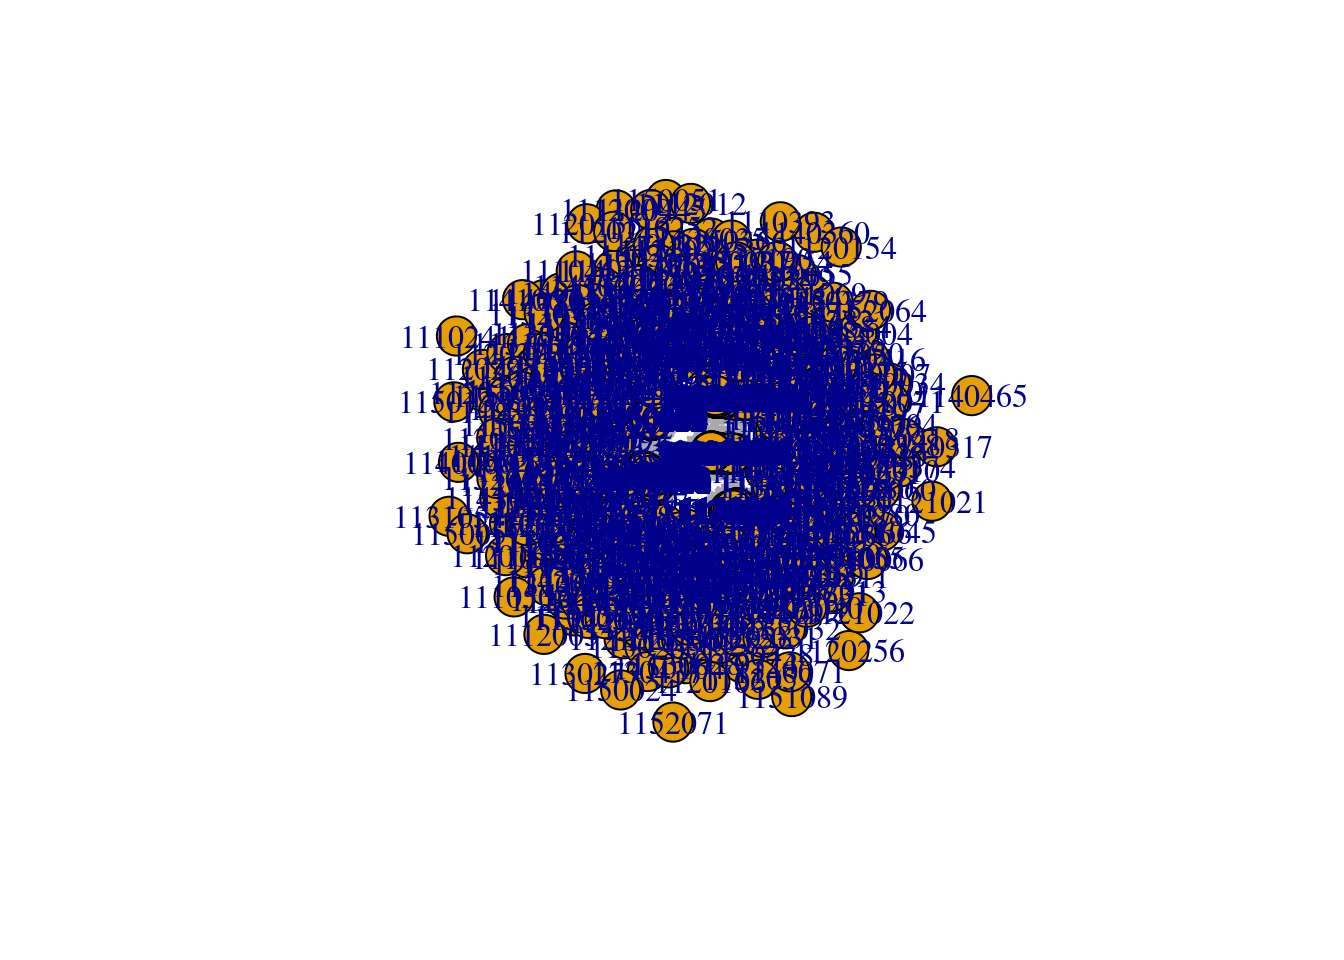
\includegraphics{03-week-1-sns-study_files/figure-latex/03-plot-raw-1} 

}

\caption{A not very nice network plot. This is what we get with the default parameters in igraph.}\label{fig:03-plot-raw}
\end{figure}

Not very nice, right? A couple of things with this plot:

\begin{enumerate}
\def\labelenumi{\arabic{enumi}.}
\item
  We are looking at all schools simultaneously, which does not make sense. So, instead of plotting \texttt{ig\_year1}, we will focus on \texttt{ig\_year1\_111}.
\item
  All the vertices have the same size, and more over, are overalaping. So, instead of using the default size, we will size the vertices by indegree using the \texttt{degree} function, and passing the vector of degrees to \texttt{vertex.size}.\footnote{Figuring out what is the optimal vertex size is a bit tricky. Without getting too technical, there's no other way of getting \emph{nice} vertex size other than just playing with different values of it. A nice solution to this is using \href{https://www.rdocumentation.org/packages/netdiffuseR/versions/1.17.0/topics/rescale_vertex_igraph}{\texttt{netdiffuseR::igraph\_vertex\_rescale}} which rescales the vertices so that these keep their aspect ratio to a predefined proportion of the screen.}
\item
  Given the number of vertices in these networks, the labels are not useful here. So we will remove them by setting \texttt{vertex.label\ =\ NA}. Moreover, we will reduce the size of the arrows' tip by setting \texttt{edge.arrow.size\ =\ 0.25}.
\item
  And finally, we will set the color of each vertex to be a function of whether the individual is hispanic or not. For this last bit we need to go a bit more of programming:
\end{enumerate}

\begin{Shaded}
\begin{Highlighting}[]
\NormalTok{col\_hispanic }\OtherTok{\textless{}{-}} \FunctionTok{V}\NormalTok{(ig\_year1\_111)}\SpecialCharTok{$}\NormalTok{hispanic }\SpecialCharTok{+} \DecValTok{1}
\NormalTok{col\_hispanic }\OtherTok{\textless{}{-}} \FunctionTok{coalesce}\NormalTok{(col\_hispanic, }\DecValTok{3}\NormalTok{) }
\NormalTok{col\_hispanic }\OtherTok{\textless{}{-}} \FunctionTok{c}\NormalTok{(}\StringTok{"steelblue"}\NormalTok{, }\StringTok{"tomato"}\NormalTok{, }\StringTok{"white"}\NormalTok{)[col\_hispanic]}
\end{Highlighting}
\end{Shaded}

Line by line, we did the following:

\begin{enumerate}
\def\labelenumi{\arabic{enumi}.}
\item
  The first line added one to all no \texttt{NA} values, so that the 0s (non-hispanic) turned to 1s and the 1s (hispanic) turned to 2s.
\item
  The second line replaced all \texttt{NA}s with the number 3, so that our vector \texttt{col\_hispanic} now ranges from 1 to 3 with no \texttt{NA}s in it.
\item
  In the last line we created a vector of colors. Essentially, what we are doing here is telling R to create a vector of length \texttt{length(col\_hispanic)} by selecting elements by index from the vector \texttt{c("steelblue",\ "tomato",\ "white")}. This way, if, for example, the first element of the vector \texttt{col\_hispanic} was a 3, our new vector of colors would have a \texttt{"white"} in it.
\end{enumerate}

To make sure we know we are right, let's print the first 10 elements of our new vector of colors together with the original \texttt{hispanic} column:

\begin{Shaded}
\begin{Highlighting}[]
\FunctionTok{cbind}\NormalTok{(}
  \AttributeTok{original =} \FunctionTok{V}\NormalTok{(ig\_year1\_111)}\SpecialCharTok{$}\NormalTok{hispanic[}\DecValTok{1}\SpecialCharTok{:}\DecValTok{10}\NormalTok{],}
  \AttributeTok{colors   =}\NormalTok{ col\_hispanic[}\DecValTok{1}\SpecialCharTok{:}\DecValTok{10}\NormalTok{]}
\NormalTok{  )}
\end{Highlighting}
\end{Shaded}

\begin{verbatim}
##       original colors     
##  [1,] "1"      "tomato"   
##  [2,] "1"      "tomato"   
##  [3,] "0"      "steelblue"
##  [4,] "1"      "tomato"   
##  [5,] "1"      "tomato"   
##  [6,] "1"      "tomato"   
##  [7,] "1"      "tomato"   
##  [8,] "1"      "tomato"   
##  [9,] "0"      "steelblue"
## [10,] "1"      "tomato"
\end{verbatim}

With our nice vector of colors, now we can pass it to \texttt{plot.igraph} (which we call implicitly by just calling \texttt{plot}), via the \texttt{vertex.color} argument:

\begin{Shaded}
\begin{Highlighting}[]
\CommentTok{\# Fancy graph}
\FunctionTok{set.seed}\NormalTok{(}\DecValTok{1}\NormalTok{)}
\FunctionTok{plot}\NormalTok{(}
\NormalTok{  ig\_year1\_111,}
  \AttributeTok{vertex.size     =} \FunctionTok{degree}\NormalTok{(ig\_year1\_111)}\SpecialCharTok{/}\DecValTok{10} \SpecialCharTok{+}\DecValTok{1}\NormalTok{,}
  \AttributeTok{vertex.label    =} \ConstantTok{NA}\NormalTok{,}
  \AttributeTok{edge.arrow.size =}\NormalTok{ .}\DecValTok{25}\NormalTok{,}
  \AttributeTok{vertex.color    =}\NormalTok{ col\_hispanic}
\NormalTok{  )}
\end{Highlighting}
\end{Shaded}

\begin{figure}
\centering
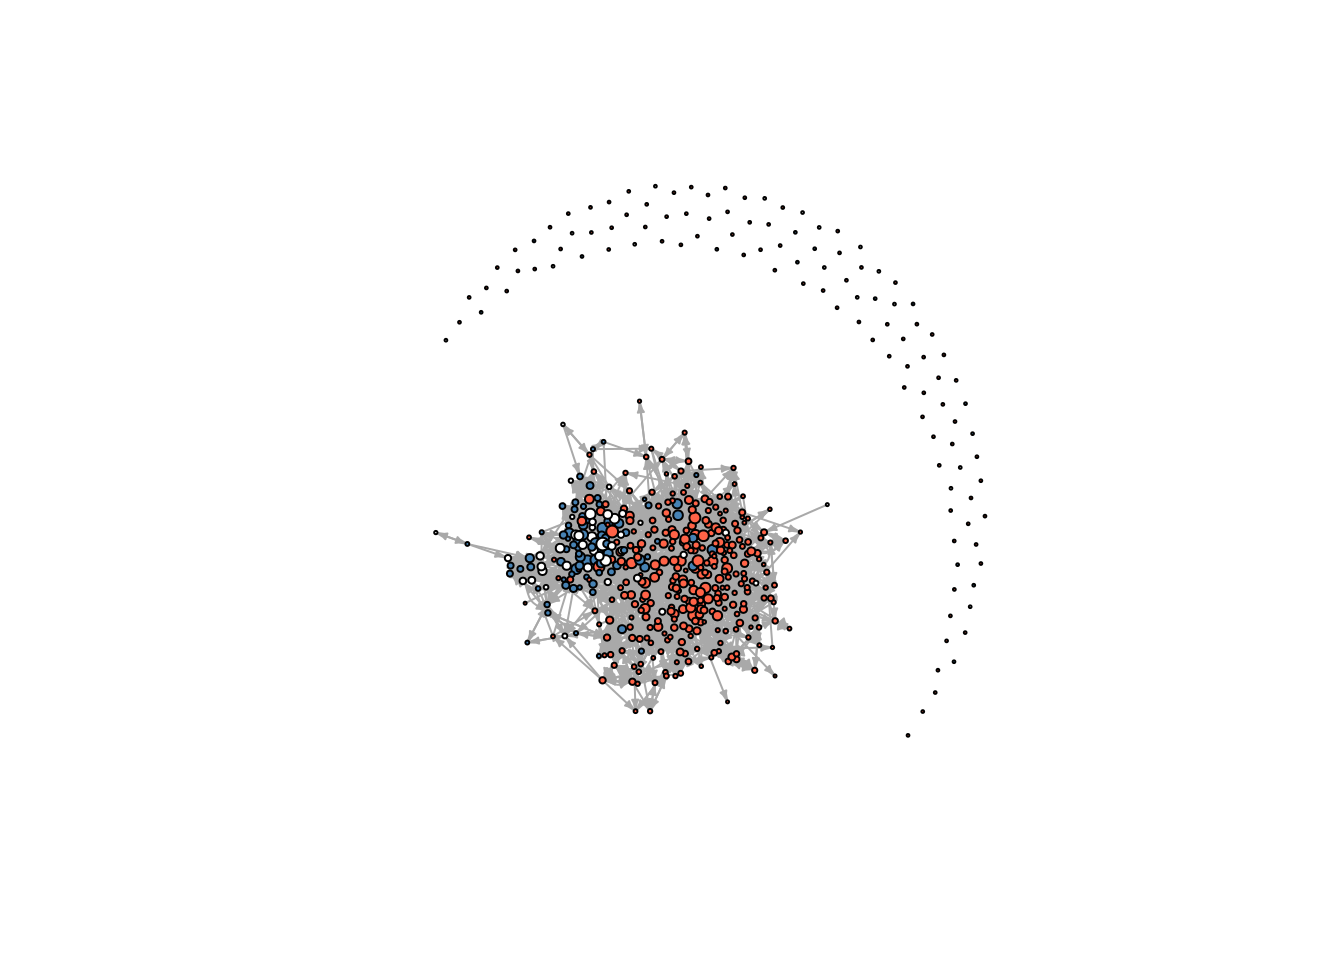
\includegraphics{03-week-1-sns-study_files/figure-latex/03-plot-neat1-1.pdf}
\caption{\label{fig:03-plot-neat1}Friends network in time 1 for school 111.}
\end{figure}

Nice! So it does look better. The only problem is that we have a lot of isolates. Let's try again by drawing the same plot without isolates. To do so we need to filter the graph, for which we will use the function \texttt{induced\_subgraph}

\begin{Shaded}
\begin{Highlighting}[]
\CommentTok{\# Which vertices are not isolates?}
\NormalTok{which\_ids }\OtherTok{\textless{}{-}} \FunctionTok{which}\NormalTok{(}\FunctionTok{degree}\NormalTok{(ig\_year1\_111, }\AttributeTok{mode =} \StringTok{"total"}\NormalTok{) }\SpecialCharTok{\textgreater{}} \DecValTok{0}\NormalTok{)}

\CommentTok{\# Getting the subgraph}
\NormalTok{ig\_year1\_111\_sub }\OtherTok{\textless{}{-}} \FunctionTok{induced\_subgraph}\NormalTok{(ig\_year1\_111, which\_ids)}

\CommentTok{\# We need to get the same subset in col\_hispanic}
\NormalTok{col\_hispanic }\OtherTok{\textless{}{-}}\NormalTok{ col\_hispanic[which\_ids]}
\end{Highlighting}
\end{Shaded}

\begin{Shaded}
\begin{Highlighting}[]
\CommentTok{\# Fancy graph}
\FunctionTok{set.seed}\NormalTok{(}\DecValTok{1}\NormalTok{)}
\FunctionTok{plot}\NormalTok{(}
\NormalTok{  ig\_year1\_111\_sub,}
  \AttributeTok{vertex.size     =} \FunctionTok{degree}\NormalTok{(ig\_year1\_111\_sub)}\SpecialCharTok{/}\DecValTok{5} \SpecialCharTok{+}\DecValTok{1}\NormalTok{,}
  \AttributeTok{vertex.label    =} \ConstantTok{NA}\NormalTok{,}
  \AttributeTok{edge.arrow.size =}\NormalTok{ .}\DecValTok{25}\NormalTok{,}
  \AttributeTok{vertex.color    =}\NormalTok{ col\_hispanic}
\NormalTok{  )}
\end{Highlighting}
\end{Shaded}

\begin{figure}
\centering
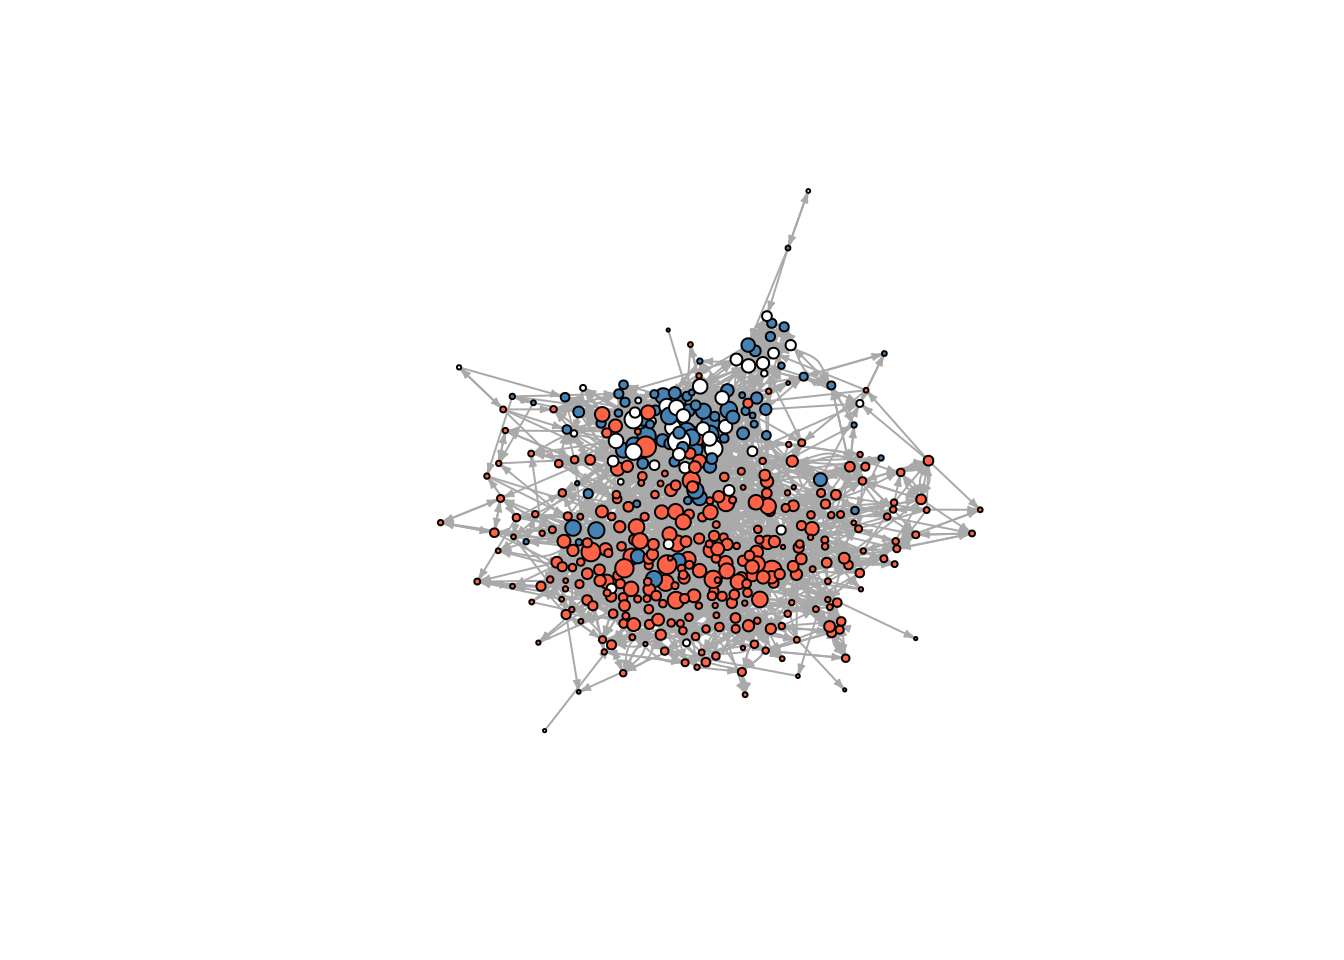
\includegraphics{03-week-1-sns-study_files/figure-latex/03-plot-neat2-1.pdf}
\caption{\label{fig:03-plot-neat2}Friends network in time 1 for school 111. The graph excludes isolates.}
\end{figure}

Now that's better! An interesting pattern that shows up is that individuals seem to cluster by whether they are hispanic or not.

We can actually write this as a function so that, instead of us copying and pasting the code \(n\) times (supposing that we want to crate a plot similar to this \(n\) times). The next subsection does that.

\hypertarget{multiple-plots}{%
\subsection{Multiple plots}\label{multiple-plots}}

When you are repeating yourself over and over again, it is a good idea to write down a sequence of commands as a function. In this case, since we will be running the same type of plot for all schools/waves, we write a function in which the only things that changes are: (a) the school id, and (b) the color of the nodes.

\begin{Shaded}
\begin{Highlighting}[]
\NormalTok{myplot }\OtherTok{\textless{}{-}} \ControlFlowTok{function}\NormalTok{(}
\NormalTok{  net,}
\NormalTok{  schoolid,}
  \AttributeTok{mindgr =} \DecValTok{1}\NormalTok{,}
  \AttributeTok{vcol   =} \StringTok{"tomato"}\NormalTok{,}
\NormalTok{  ...) \{}
  
  \CommentTok{\# Creating a subgraph}
\NormalTok{  subnet }\OtherTok{\textless{}{-}} \FunctionTok{induced\_subgraph}\NormalTok{(}
\NormalTok{    net,}
    \FunctionTok{which}\NormalTok{(}\FunctionTok{degree}\NormalTok{(net, }\AttributeTok{mode =} \StringTok{"all"}\NormalTok{) }\SpecialCharTok{\textgreater{}=}\NormalTok{ mindgr }\SpecialCharTok{\&} \FunctionTok{V}\NormalTok{(net)}\SpecialCharTok{$}\NormalTok{school }\SpecialCharTok{==}\NormalTok{ schoolid)}
\NormalTok{  )}
  
  \CommentTok{\# Fancy graph}
  \FunctionTok{set.seed}\NormalTok{(}\DecValTok{1}\NormalTok{)}
  \FunctionTok{plot}\NormalTok{(}
\NormalTok{    subnet,}
    \AttributeTok{vertex.size     =} \FunctionTok{degree}\NormalTok{(subnet)}\SpecialCharTok{/}\DecValTok{5}\NormalTok{,}
    \AttributeTok{vertex.label    =} \ConstantTok{NA}\NormalTok{,}
    \AttributeTok{edge.arrow.size =}\NormalTok{ .}\DecValTok{25}\NormalTok{,}
    \AttributeTok{vertex.color    =}\NormalTok{ vcol,}
\NormalTok{    ...}
\NormalTok{    )}
\NormalTok{\}}
\end{Highlighting}
\end{Shaded}

The function definition:

\begin{enumerate}
\def\labelenumi{\arabic{enumi}.}
\item
  The \texttt{myplot\ \textless{}-\ function({[}arguments{]})\ \{{[}body\ of\ the\ function{]}\}} tells R that we are going to create a function called \texttt{myplot}.
\item
  In the arguments part, we are declaring 4 specific arguments: \texttt{net}, \texttt{schoolid}, \texttt{mindgr}, and \texttt{vcol}. These are an igraph object, the school id, the minimum degree that a vertex must have to be included in the plot, and the color of the vertices. Notice that, as a difference from other programming languages, in R we don't need to declare the types that these objects are.
\item
  The elipsis object, \texttt{...}, is a special object in R that allows us passing other arguments without us specifying which. In our case, if you take a look at the \texttt{plot} bit of the body of the function, you will see that we also added \texttt{...}; this means that whatever other arguments (different from the ones that we explicitly defined) are passed to the function, these will be passed to the function \texttt{plot}, moreover, to the \texttt{plot.gexf} function (since the \texttt{subnet} object is actually an igraph object). In practice, this implies that we can, for example, set the argument \texttt{edge.arrow.size} when calling \texttt{myplot}, even though we did not included it in the function definition! (See \texttt{?dotsMethods} in R for more details).
\end{enumerate}

In the following lines of code, using our new function, we will plot each schools' network in the same plotting device (window) with the help of the \texttt{par} function, and add legend with the \texttt{legend}:

\begin{Shaded}
\begin{Highlighting}[]
\CommentTok{\# Plotting all together}
\NormalTok{oldpar }\OtherTok{\textless{}{-}} \FunctionTok{par}\NormalTok{(}\AttributeTok{no.readonly =} \ConstantTok{TRUE}\NormalTok{)}
\FunctionTok{par}\NormalTok{(}\AttributeTok{mfrow =} \FunctionTok{c}\NormalTok{(}\DecValTok{2}\NormalTok{, }\DecValTok{3}\NormalTok{), }\AttributeTok{mai =} \FunctionTok{rep}\NormalTok{(}\DecValTok{0}\NormalTok{, }\DecValTok{4}\NormalTok{), }\AttributeTok{oma=} \FunctionTok{c}\NormalTok{(}\DecValTok{1}\NormalTok{, }\DecValTok{0}\NormalTok{, }\DecValTok{0}\NormalTok{, }\DecValTok{0}\NormalTok{))}
\FunctionTok{myplot}\NormalTok{(ig\_year1, }\DecValTok{111}\NormalTok{, }\AttributeTok{vcol =} \StringTok{"tomato"}\NormalTok{)}
\FunctionTok{myplot}\NormalTok{(ig\_year1, }\DecValTok{112}\NormalTok{, }\AttributeTok{vcol =} \StringTok{"steelblue"}\NormalTok{)}
\FunctionTok{myplot}\NormalTok{(ig\_year1, }\DecValTok{113}\NormalTok{, }\AttributeTok{vcol =} \StringTok{"black"}\NormalTok{)}
\FunctionTok{myplot}\NormalTok{(ig\_year1, }\DecValTok{114}\NormalTok{, }\AttributeTok{vcol =} \StringTok{"gold"}\NormalTok{)}
\FunctionTok{myplot}\NormalTok{(ig\_year1, }\DecValTok{115}\NormalTok{, }\AttributeTok{vcol =} \StringTok{"white"}\NormalTok{)}
\FunctionTok{par}\NormalTok{(oldpar)}

\CommentTok{\# A fancy legend}
\FunctionTok{legend}\NormalTok{(}
  \StringTok{"bottomright"}\NormalTok{,}
  \AttributeTok{legend =} \FunctionTok{c}\NormalTok{(}\DecValTok{111}\NormalTok{, }\DecValTok{112}\NormalTok{, }\DecValTok{113}\NormalTok{, }\DecValTok{114}\NormalTok{, }\DecValTok{115}\NormalTok{),}
  \AttributeTok{pt.bg  =} \FunctionTok{c}\NormalTok{(}\StringTok{"tomato"}\NormalTok{, }\StringTok{"steelblue"}\NormalTok{, }\StringTok{"black"}\NormalTok{, }\StringTok{"gold"}\NormalTok{, }\StringTok{"white"}\NormalTok{),}
  \AttributeTok{pch    =} \DecValTok{21}\NormalTok{,}
  \AttributeTok{cex    =} \DecValTok{1}\NormalTok{,}
  \AttributeTok{bty    =} \StringTok{"n"}\NormalTok{,}
  \AttributeTok{title  =} \StringTok{"School"}
\NormalTok{  )}
\end{Highlighting}
\end{Shaded}

\begin{figure}
\centering
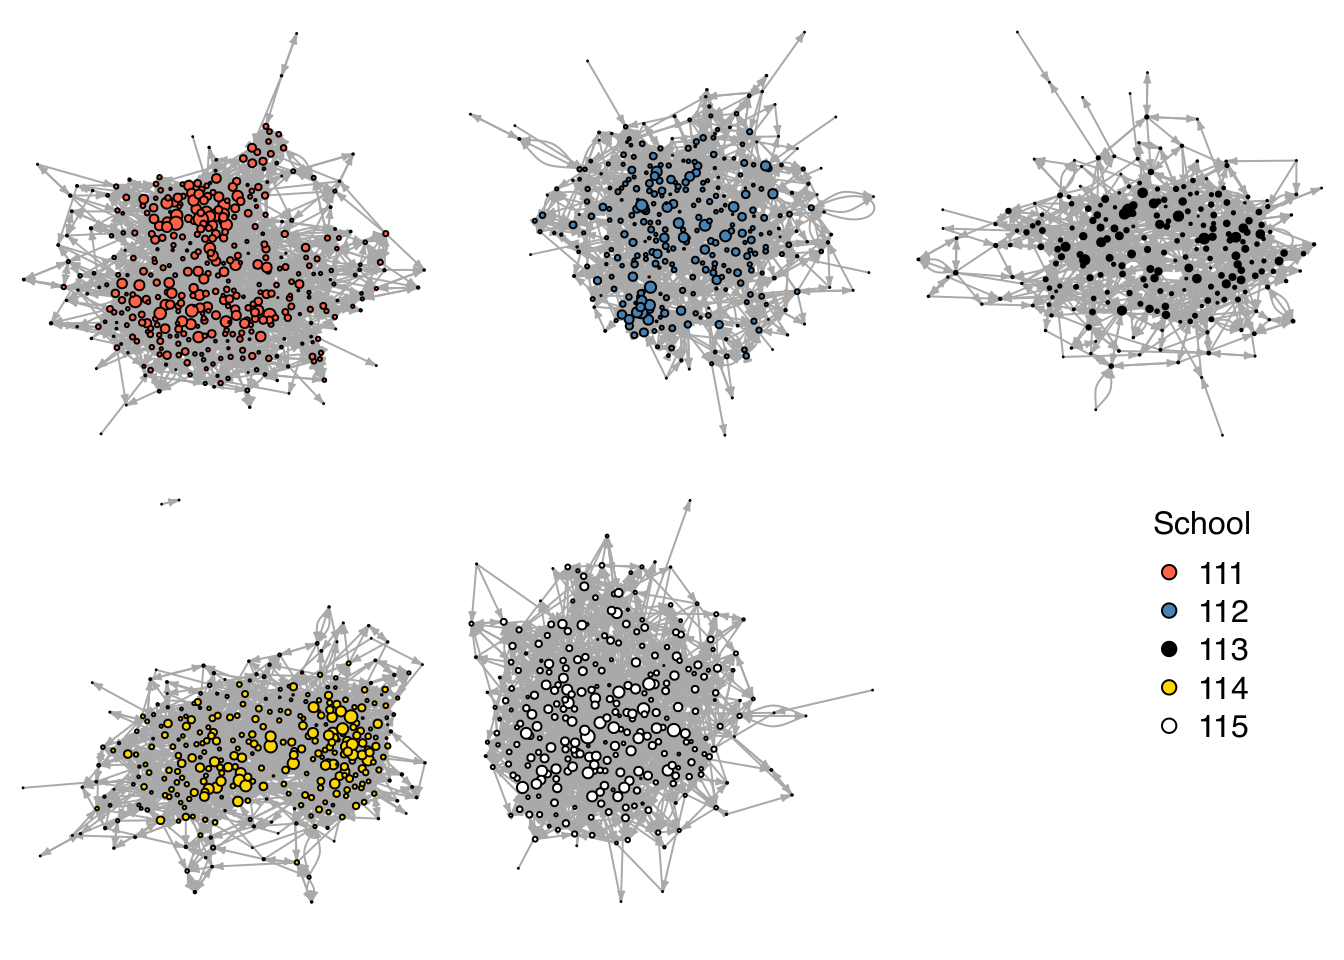
\includegraphics{03-week-1-sns-study_files/figure-latex/03-myplot-call-1.pdf}
\caption{\label{fig:03-myplot-call}All 5 schools in time 1. Again, the graphs exclude isolates.}
\end{figure}

So what happend here?

\begin{itemize}
\item
  \texttt{oldpar\ \textless{}-\ par(no.readonly\ =\ TRUE)} This line stores the current parameters for plotting. Since we are going to be changing them, we better make sure we are able to go back!.
\item
  \texttt{par(mfrow\ =\ c(2,\ 3),\ mai\ =\ rep(0,\ 4),\ oma=rep(0,\ 4))} Here we are setting various things at the same time. \texttt{mfrow} specifies how many \emph{figures} will be drawn and in what order, in particular, we are asking the plotting device to allow for 2*3 = 6 plots organized in 2 rows and 3 columns, and these will be drawn by row.

  \texttt{mai} specifies the size of the margins in inches. Setting all margins equal to zero (which is what we are doing now) gives more space to the network itself. The same is true for \texttt{oma}. See \texttt{?par} for more info.
\item
  \texttt{myplot(ig\_year1,\ ...)} This is simply calling our plotting function. The neat part of this is that, since we set \texttt{mfrow\ =\ c(2,\ 3)}, R takes care of \emph{distributing} the plots in the device.
\item
  \texttt{par(oldpar)} This line allows us to restore the plotting parameters.
\end{itemize}

\hypertarget{statistical-tests}{%
\section{Statistical tests}\label{statistical-tests}}

\hypertarget{is-nomination-number-correlated-with-indegree}{%
\subsection{Is nomination number correlated with indegree?}\label{is-nomination-number-correlated-with-indegree}}

Hypothesis: Individuals that on average are among the first nominations of their peers are more popular

\begin{Shaded}
\begin{Highlighting}[]
\CommentTok{\# Getting all the data in long format}
\NormalTok{edgelist }\OtherTok{\textless{}{-}} \FunctionTok{as\_long\_data\_frame}\NormalTok{(ig\_year1) }\SpecialCharTok{\%\textgreater{}\%}
\NormalTok{  as\_tibble}

\CommentTok{\# Computing indegree (again) and average nomination number}
\CommentTok{\# Include "On a scale from one to five how close do you feel"}
\CommentTok{\# Also for egocentric friends (A. Friends)}
\NormalTok{indeg\_nom\_cor }\OtherTok{\textless{}{-}} \FunctionTok{group\_by}\NormalTok{(edgelist, to, to\_name, to\_school) }\SpecialCharTok{\%\textgreater{}\%}
  \FunctionTok{summarise}\NormalTok{(}
    \AttributeTok{indeg   =} \FunctionTok{length}\NormalTok{(nnom),}
    \AttributeTok{nom\_avg =} \DecValTok{1}\SpecialCharTok{/}\FunctionTok{mean}\NormalTok{(nnom)}
\NormalTok{  ) }\SpecialCharTok{\%\textgreater{}\%}
  \FunctionTok{rename}\NormalTok{(}
    \AttributeTok{school =}\NormalTok{ to\_school}
\NormalTok{  )}

\NormalTok{indeg\_nom\_cor}
\end{Highlighting}
\end{Shaded}

\begin{verbatim}
## # A tibble: 1,561 x 5
## # Groups:   to, to_name [1,561]
##       to to_name school indeg nom_avg
##    <dbl> <chr>    <int> <int>   <dbl>
##  1     2 1110002    111    22   0.222
##  2     3 1110007    111     7   0.175
##  3     4 1110013    111     6   0.171
##  4     5 1110014    111    19   0.134
##  5     6 1110015    111     3   0.15 
##  6     7 1110020    111     6   0.154
##  7     9 1110025    111     6   0.214
##  8    10 1110027    111    13   0.220
##  9    11 1110029    111    14   0.131
## 10    12 1110030    111     6   0.222
## # ... with 1,551 more rows
\end{verbatim}

\begin{Shaded}
\begin{Highlighting}[]
\CommentTok{\# Using pearson\textquotesingle{}s correlation}
\FunctionTok{with}\NormalTok{(indeg\_nom\_cor, }\FunctionTok{cor.test}\NormalTok{(indeg, nom\_avg))}
\end{Highlighting}
\end{Shaded}

\begin{verbatim}
## 
##  Pearson's product-moment correlation
## 
## data:  indeg and nom_avg
## t = -12.254, df = 1559, p-value < 2.2e-16
## alternative hypothesis: true correlation is not equal to 0
## 95 percent confidence interval:
##  -0.3409964 -0.2504653
## sample estimates:
##        cor 
## -0.2963965
\end{verbatim}

\begin{Shaded}
\begin{Highlighting}[]
\FunctionTok{save.image}\NormalTok{(}\StringTok{"03.rda"}\NormalTok{)}
\end{Highlighting}
\end{Shaded}

\hypertarget{exponential-random-graph-models}{%
\chapter{Exponential Random Graph Models}\label{exponential-random-graph-models}}

I strongly suggest reading the vignette included in the \texttt{ergm} R package

\begin{Shaded}
\begin{Highlighting}[]
\FunctionTok{vignette}\NormalTok{(}\StringTok{"ergm"}\NormalTok{, }\AttributeTok{package=}\StringTok{"ergm"}\NormalTok{)}
\end{Highlighting}
\end{Shaded}

So what are ERGMs anyway\ldots{}

\begin{quote}
The purpose of ERGMs, in a nutshell, is to describe parsimoniously the local selection forces
that shape the global structure of a network. To this end, a network dataset, like those
depicted in Figure 1, may be considered like the response in a regression model, where the
predictors are things like ``propensity for individuals of the same sex to form partnerships'' or
``propensity for individuals to form triangles of partnerships.'' In Figure 1(b), for example, it
is evident that the individual nodes appear to cluster in groups of the same numerical labels
(which turn out to be students' grades, 7 through 12); thus, an ERGM can help us quantify
the strength of this intra-group effect.

--- (\protect\hyperlink{ref-Hunter2008}{David R. Hunter et al. 2008})
\end{quote}

\begin{figure}
\centering
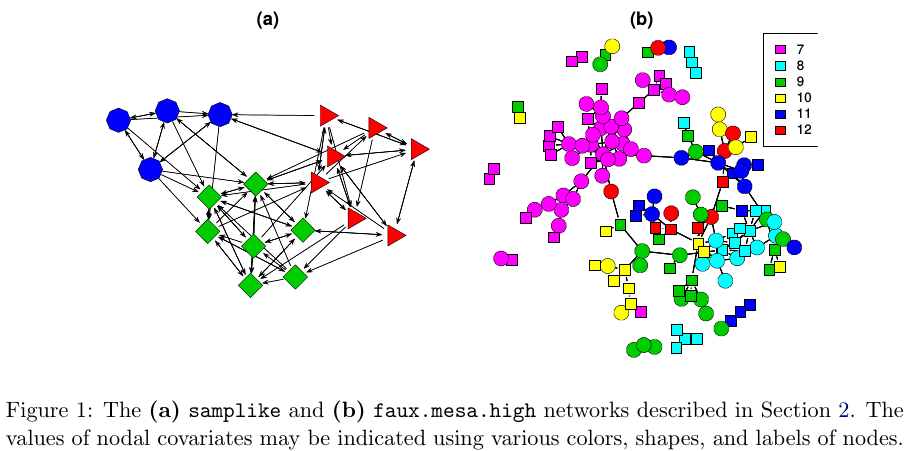
\includegraphics{hunter2008.png}
\caption{Source: Hunter et al.~(2008)}
\end{figure}

The distribution of \(\mathbf{Y}\) can be parameterized in the form

\[
\mbox{Pr}\left(\mathbf{Y}=\mathbf{y}|\theta, \mathcal{Y}\right) = \frac{\mbox{exp}\left\{\theta^{\mbox{T}}\mathbf{g}(\mathbf{y})\right\}}{\kappa\left(\theta, \mathcal{Y}\right)},\quad\mathbf{y}\in\mathcal{Y}
\label{eq:04-1}
\]

Where \(\theta\in\Omega\subset\mathbb{R}^q\) is the vector of model coefficients and \(\mathbf{g}(\mathbf{y})\) is a \emph{q}-vector of statistics based on the adjacency matrix \(\mathbf{y}\).

Model \eqref{eq:04-1} may be expanded by replacing \(\mathbf{g}(\mathbf{y})\) with \(\mathbf{g}(\mathbf{y}, \mathbf{X})\) to allow for additional covariate information \(\mathbf{X}\) about the network. The denominator,

\[
\kappa\left(\theta,\mathcal{Y}\right) = \sum_{\mathbf{y}\in\mathcal{Y}}\mbox{exp}\left\{\theta^{\mbox{T}}\mathbf{g}(\mathbf{y})\right\}
\]

Is the normalizing factor that ensures that equation \eqref{eq:04-1} is a legitimate probability distribution. Even after fixing \(\mathcal{Y}\) to be all the networks that have size \(n\), the size of \(\mathcal{Y}\) makes this type of models hard to estimate as there are \(N = 2^{n(n-1)}\) possible networks! (\protect\hyperlink{ref-Hunter2008}{David R. Hunter et al. 2008})

Recent developments include new forms of dependency structures, to take into account more general neighborhood effects. These models relax the one-step Markovian dependence assumptions, allowing investigation of longer range configurations, such as longer paths in the network or larger cycles (Pattison and Robins 2002). Models for bipartite (Faust and Skvoretz 1999) and tripartite (Mische and Robins 2000) network structures have also been developed. (\protect\hyperlink{ref-Hunter2008}{David R. Hunter et al. 2008, 9})

\hypertarget{a-naive-example}{%
\subsection{A naive example}\label{a-naive-example}}

In the simplest case, ergm is equivalent to a logistic regression

\begin{Shaded}
\begin{Highlighting}[]
\FunctionTok{library}\NormalTok{(ergm)}
\end{Highlighting}
\end{Shaded}

\begin{verbatim}
## Loading required package: network
\end{verbatim}

\begin{verbatim}
## network: Classes for Relational Data
## Version 1.16.1 created on 2020-10-06.
## copyright (c) 2005, Carter T. Butts, University of California-Irvine
##                     Mark S. Handcock, University of California -- Los Angeles
##                     David R. Hunter, Penn State University
##                     Martina Morris, University of Washington
##                     Skye Bender-deMoll, University of Washington
##  For citation information, type citation("network").
##  Type help("network-package") to get started.
\end{verbatim}

\begin{verbatim}
## 
## ergm: version 3.11.0, created on 2020-10-14
## Copyright (c) 2020, Mark S. Handcock, University of California -- Los Angeles
##                     David R. Hunter, Penn State University
##                     Carter T. Butts, University of California -- Irvine
##                     Steven M. Goodreau, University of Washington
##                     Pavel N. Krivitsky, UNSW Sydney
##                     Martina Morris, University of Washington
##                     with contributions from
##                     Li Wang
##                     Kirk Li, University of Washington
##                     Skye Bender-deMoll, University of Washington
##                     Chad Klumb
##                     Michał Bojanowski, Kozminski University
##                     Ben Bolker
## Based on "statnet" project software (statnet.org).
## For license and citation information see statnet.org/attribution
## or type citation("ergm").
\end{verbatim}

\begin{verbatim}
## NOTE: Versions before 3.6.1 had a bug in the implementation of the bd()
## constraint which distorted the sampled distribution somewhat. In
## addition, Sampson's Monks datasets had mislabeled vertices. See the
## NEWS and the documentation for more details.
\end{verbatim}

\begin{verbatim}
## NOTE: Some common term arguments pertaining to vertex attribute and
## level selection have changed in 3.10.0. See terms help for more
## details. Use 'options(ergm.term=list(version="3.9.4"))' to use old
## behavior.
\end{verbatim}

\begin{Shaded}
\begin{Highlighting}[]
\FunctionTok{data}\NormalTok{(}\StringTok{"sampson"}\NormalTok{)}

\NormalTok{samplike}
\end{Highlighting}
\end{Shaded}

\begin{verbatim}
##  Network attributes:
##   vertices = 18 
##   directed = TRUE 
##   hyper = FALSE 
##   loops = FALSE 
##   multiple = FALSE 
##   total edges= 88 
##     missing edges= 0 
##     non-missing edges= 88 
## 
##  Vertex attribute names: 
##     cloisterville group vertex.names 
## 
##  Edge attribute names: 
##     nominations
\end{verbatim}

\begin{Shaded}
\begin{Highlighting}[]
\NormalTok{y }\OtherTok{\textless{}{-}} \FunctionTok{sort}\NormalTok{(}\FunctionTok{as.vector}\NormalTok{(}\FunctionTok{as.matrix}\NormalTok{(samplike)))[}\SpecialCharTok{{-}}\FunctionTok{c}\NormalTok{(}\DecValTok{1}\SpecialCharTok{:}\DecValTok{18}\NormalTok{)]}
\FunctionTok{glm}\NormalTok{(y}\SpecialCharTok{\textasciitilde{}}\DecValTok{1}\NormalTok{, }\AttributeTok{family=}\FunctionTok{binomial}\NormalTok{(}\StringTok{"logit"}\NormalTok{))}
\end{Highlighting}
\end{Shaded}

\begin{verbatim}
## 
## Call:  glm(formula = y ~ 1, family = binomial("logit"))
## 
## Coefficients:
## (Intercept)  
##     -0.9072  
## 
## Degrees of Freedom: 305 Total (i.e. Null);  305 Residual
## Null Deviance:       367.2 
## Residual Deviance: 367.2     AIC: 369.2
\end{verbatim}

\begin{Shaded}
\begin{Highlighting}[]
\FunctionTok{ergm}\NormalTok{(samplike }\SpecialCharTok{\textasciitilde{}}\NormalTok{ edges)}
\end{Highlighting}
\end{Shaded}

\begin{verbatim}
## Starting maximum pseudolikelihood estimation (MPLE):
\end{verbatim}

\begin{verbatim}
## Evaluating the predictor and response matrix.
\end{verbatim}

\begin{verbatim}
## Maximizing the pseudolikelihood.
\end{verbatim}

\begin{verbatim}
## Finished MPLE.
\end{verbatim}

\begin{verbatim}
## Stopping at the initial estimate.
\end{verbatim}

\begin{verbatim}
## Evaluating log-likelihood at the estimate.
\end{verbatim}

\begin{verbatim}
## 
## Call:
## ergm(formula = samplike ~ edges)
## 
## 
## MLE Coefficients:
##   edges  
## -0.9072
\end{verbatim}

\begin{Shaded}
\begin{Highlighting}[]
\NormalTok{pr }\OtherTok{\textless{}{-}} \FunctionTok{mean}\NormalTok{(y)}
\FunctionTok{log}\NormalTok{(pr) }\SpecialCharTok{{-}} \FunctionTok{log}\NormalTok{(}\DecValTok{1}\SpecialCharTok{{-}}\NormalTok{pr) }\CommentTok{\# Logit function}
\end{Highlighting}
\end{Shaded}

\begin{verbatim}
## [1] -0.9071582
\end{verbatim}

\begin{Shaded}
\begin{Highlighting}[]
\FunctionTok{qlogis}\NormalTok{(pr)}
\end{Highlighting}
\end{Shaded}

\begin{verbatim}
## [1] -0.9071582
\end{verbatim}

\hypertarget{estimation-of-ergms}{%
\section{Estimation of ERGMs}\label{estimation-of-ergms}}

The ultimate goal is to be able to do statistical inference on the proposed model. In a \emph{normal} setting, we would be able to use Maximum-Likelihood-Estimation (MLE) which basically consists on finding the model parameters \(\theta\) that, given the observed data, maximizes the likelihood of the model. Such is usually done by applying \href{https://en.wikipedia.org/wiki/Newton\%27s_method_in_optimization}{Newton's method} which requires been able to compute the log-likelihood of the model. This is a bit more complicated in ERGMs.

In the case of ERGMs, since part of the likelihood involves a normalizing constant that is a function of all possible networks, this is not as straight forward as it is in the regular setting. This is why we rely on simulations.

In \texttt{statnet}, the default estimation method is based on a method proposed by (\protect\hyperlink{ref-Geyer1992}{Geyer and Thompson 1992}), Markov-Chain MLE, which uses Markov-Chain Monte Carlo for simulating networks and a modified version of the Newton-Raphson algorihm to do the paremeter estimation part.

The idea of MC-MLE for this family of statistical models is the fact that the expectation of normalizing constant ratios can be approximated using the law of large numbers. In particular, the following:

\[
\begin{aligned}
\frac{\kappa\left(\theta,\mathcal{Y}\right)}{\kappa\left(\theta_0,\mathcal{Y}\right)} & = %
  \frac{%
    \sum_{\mathbf{y}\in\mathcal{Y}}\mbox{exp}\left\{\theta^{\mbox{T}}\mathbf{g}(\mathbf{y})\right\}}{ %
    \sum_{\mathbf{y}\in\mathcal{Y}}\mbox{exp}\left\{\theta_0^{\mbox{T}}\mathbf{g}(\mathbf{y})\right\}
  } \\
& = \sum_{\mathbf{y}\in\mathcal{Y}}\left( %
  \frac{1}{%
    \sum_{\mathbf{y}\in\mathcal{Y}\mbox{exp}\left\{\theta_0^{\mbox{T}}\mathbf{g}(\mathbf{y})\right\}}%
  } \times %
  \mbox{exp}\left\{\theta^{\mbox{T}}\mathbf{g}(\mathbf{y})\right\} %
  \right) \\
& = \sum_{\mathbf{y}\in\mathcal{Y}}\left( %
  \frac{\mbox{exp}\left\{\theta_0^{\mbox{T}}\mathbf{g}(\mathbf{y})\right\}}{%
    \sum_{\mathbf{y}\in\mathcal{Y}\mbox{exp}\left\{\theta_0^{\mbox{T}}\mathbf{g}(\mathbf{y})\right\}}%
  } \times %
  \mbox{exp}\left\{(\theta - \theta_0)^{\mbox{T}}\mathbf{g}(\mathbf{y})\right\} %
  \right) \\
& = \sum_{\mathbf{y}\in\mathcal{Y}}\left( %
  \mbox{Pr}\left(Y = y|\mathcal{Y}, \theta_0\right) \times %
  \mbox{exp}\left\{(\theta - \theta_0)^{\mbox{T}}\mathbf{g}(\mathbf{y})\right\} %
  \right) \\
& = \mbox{E}_{\theta_0}\left(\mbox{exp}\left\{(\theta - \theta_0)^{\mbox{T}}\mathbf{g}(\mathbf{y})\right\} \right)
\end{aligned}
\]

The final line can be approximated by the law of large numbers. In particular, the MC-MLE algorithm uses this fact to maximize the ratio of log-likelihoods. The objective function can be approximated by simulating \(m\) networks from the distribution with parameter \(\theta_0\):

\[
l(\theta) - l(\theta_0) \approx (\theta - \theta_0)^{\mbox{T}}\mathbf{g}(\mathbf{y}_{obs}) - 
\mbox{log}{\left[\frac{1}{m}\sum_{i = 1}^m\mbox{exp}\left\{(\theta-\theta_0)^{\mbox{T}}\right\}\mathbf{g}(\mathbf{Y}_i)\right]}
\]

For more details see (\protect\hyperlink{ref-Hunter2008}{David R. Hunter et al. 2008}). A sketch of the algorithm follows:

\begin{enumerate}
\def\labelenumi{\arabic{enumi}.}
\item
  Initialize the algorithm with an initial guess of \(\theta\), call it \(\theta^{(t)}\) (must be a rather OK guess)
\item
  While (no convergence) do:

  \begin{enumerate}
  \def\labelenumii{\alph{enumii}.}
  \item
    Using \(\theta^{(t)}\), simulate \(M\) networks by means of small changes in the \(\mathbf{Y}_{obs}\) (the observed network). This part is done by using an importance-sampling method which weights each proposed network by it's likelihood conditional on \(\theta^{(t)}\)
  \item
    With the networks simulated, we can do the Newton step to update the parameter \(\theta^{(t)}\) (this is the iteration part in the \texttt{ergm} package): \(\theta^{(t)}\to\theta^{(t+1)}\).
  \item
    If convergence has been reach (which usually means that \(\theta^{(t)}\) and \(\theta^{(t + 1)}\) are not very different), then stop, otherwise, go to step a.
  \end{enumerate}
\end{enumerate}

For more details see (\protect\hyperlink{ref-lusher2012}{Lusher, Koskinen, and Robins 2012}; \protect\hyperlink{ref-admiraal2006}{Admiraal and Handcock 2006}; \protect\hyperlink{ref-Snijders2002}{T. A. Snijders 2002}; \protect\hyperlink{ref-Wang2009}{Wang et al. 2009}) provides details on the algorithm used by PNet (which is the same as the one used in \texttt{RSiena}). (\protect\hyperlink{ref-lusher2012}{Lusher, Koskinen, and Robins 2012}) provides a short discussion on differences between \texttt{ergm} and \texttt{PNet}.

\hypertarget{the-ergm-package}{%
\section{\texorpdfstring{The \texttt{ergm} package}{The ergm package}}\label{the-ergm-package}}

The \texttt{ergm} R package (\protect\hyperlink{ref-R-ergm}{Handcock et al. 2017})

From the previous section:\footnote{You can download the 03.rda file from \href{https://github.com/gvegayon/appliedsnar}{this link}.}

\begin{Shaded}
\begin{Highlighting}[]
\FunctionTok{library}\NormalTok{(igraph)}
\FunctionTok{library}\NormalTok{(magrittr)}
\FunctionTok{library}\NormalTok{(dplyr)}

\FunctionTok{load}\NormalTok{(}\StringTok{"03.rda"}\NormalTok{)}
\end{Highlighting}
\end{Shaded}

In this section we will use the \texttt{ergm} package (from the \texttt{statnet} suit of packages (\protect\hyperlink{ref-R-statnet}{Handcock et al. 2016})) suit, and the \texttt{intergraph} (\protect\hyperlink{ref-R-intergraph}{Bojanowski 2015}) package. The latter provides functions to go back and forth between \texttt{igraph} and \texttt{network} objects from the \texttt{igraph} and \texttt{network} packages respectively\footnote{Yes, the classes have the same name as the packages.}

\begin{Shaded}
\begin{Highlighting}[]
\FunctionTok{library}\NormalTok{(ergm)}
\FunctionTok{library}\NormalTok{(intergraph)}
\end{Highlighting}
\end{Shaded}

As a rather important side note, the order in which R packages are loaded matters. Why is this important to mention now? Well, it turns out that at least a couple of functions in the \texttt{network} package have the same name of some functions in the \texttt{igraph} package. When the \texttt{ergm} package is loaded, since it depends on \texttt{network}, it will load the \texttt{network} package first, which will \emph{mask} some functions in \texttt{igraph}. This becomes evident once you load \texttt{ergm} after loading \texttt{igraph}:

\begin{verbatim}
The following objects are masked from ‘package:igraph’:

  add.edges, add.vertices, %c%, delete.edges, delete.vertices, get.edge.attribute, get.edges,
  get.vertex.attribute, is.bipartite, is.directed, list.edge.attributes, list.vertex.attributes, %s%,
  set.edge.attribute, set.vertex.attribute
\end{verbatim}

What are the implications of this? If you call the function \texttt{list.edge.attributes} for an object of class \texttt{igraph} R will return an error as the first function that matches that name comes from the \texttt{network} package! To avoid this you can use the double colon notation:

\begin{Shaded}
\begin{Highlighting}[]
\NormalTok{igraph}\SpecialCharTok{::}\FunctionTok{list.edge.attributes}\NormalTok{(my\_igraph\_object)}
\NormalTok{network}\SpecialCharTok{::}\FunctionTok{list.edge.attributes}\NormalTok{(my\_network\_object)}
\end{Highlighting}
\end{Shaded}

Anyway\ldots{} Using the \texttt{asNetwork} function, we can coerce the igraph object into a network object so we can use it with the \texttt{ergm} function:

\begin{Shaded}
\begin{Highlighting}[]
\CommentTok{\# Creating the new network}
\NormalTok{network\_111 }\OtherTok{\textless{}{-}}\NormalTok{ intergraph}\SpecialCharTok{::}\FunctionTok{asNetwork}\NormalTok{(ig\_year1\_111)}

\CommentTok{\# Running a simple ergm (only fitting edge count)}
\FunctionTok{ergm}\NormalTok{(network\_111 }\SpecialCharTok{\textasciitilde{}}\NormalTok{ edges)}
\end{Highlighting}
\end{Shaded}

\begin{verbatim}
## [1] "Warning:  This network contains loops"
## [1] "Warning:  This network contains loops"
\end{verbatim}

\begin{verbatim}
## Starting maximum pseudolikelihood estimation (MPLE):
\end{verbatim}

\begin{verbatim}
## Evaluating the predictor and response matrix.
\end{verbatim}

\begin{verbatim}
## Maximizing the pseudolikelihood.
\end{verbatim}

\begin{verbatim}
## Finished MPLE.
\end{verbatim}

\begin{verbatim}
## Stopping at the initial estimate.
\end{verbatim}

\begin{verbatim}
## Evaluating log-likelihood at the estimate.
\end{verbatim}

\begin{verbatim}
## 
## MLE Coefficients:
##  edges  
## -4.734
\end{verbatim}

So what happened here! We got a warning. It turns out that our network has loops (didn't thought about it before!). Let's take a look on that with the \texttt{which\_loop} function

\begin{Shaded}
\begin{Highlighting}[]
\FunctionTok{E}\NormalTok{(ig\_year1\_111)[}\FunctionTok{which\_loop}\NormalTok{(ig\_year1\_111)]}
\end{Highlighting}
\end{Shaded}

\begin{verbatim}
## + 1/2638 edge from eecafe0 (vertex names):
## [1] 1110111->1110111
\end{verbatim}

We can get rid of these using the \texttt{igraph::-.igraph}. Moreover, just to illustrate how it can be done, let's get rid of the isolates using the same operator

\begin{Shaded}
\begin{Highlighting}[]
\CommentTok{\# Creating the new network}
\NormalTok{network\_111 }\OtherTok{\textless{}{-}}\NormalTok{ ig\_year1\_111}

\CommentTok{\# Removing loops}
\NormalTok{network\_111 }\OtherTok{\textless{}{-}}\NormalTok{ network\_111 }\SpecialCharTok{{-}} \FunctionTok{E}\NormalTok{(network\_111)[}\FunctionTok{which}\NormalTok{(}\FunctionTok{which\_loop}\NormalTok{(network\_111))]}

\CommentTok{\# Removing isolates}
\NormalTok{network\_111 }\OtherTok{\textless{}{-}}\NormalTok{ network\_111 }\SpecialCharTok{{-}} \FunctionTok{which}\NormalTok{(}\FunctionTok{degree}\NormalTok{(network\_111, }\AttributeTok{mode =} \StringTok{"all"}\NormalTok{) }\SpecialCharTok{==} \DecValTok{0}\NormalTok{)}

\CommentTok{\# Converting the network}
\NormalTok{network\_111 }\OtherTok{\textless{}{-}}\NormalTok{ intergraph}\SpecialCharTok{::}\FunctionTok{asNetwork}\NormalTok{(network\_111)}
\end{Highlighting}
\end{Shaded}

\texttt{asNetwork(simplify(ig\_year1\_111))}
\texttt{ig\_year1\_111\ \%\textgreater{}\%\ simplify\ \%\textgreater{}\%\ asNetwork}

A problem that we have on this data is the fact that some vertices have
missing values in the variables \texttt{hispanic}, \texttt{female1}, and \texttt{eversmk1}. For now,
we will proceed by imputing values based on the avareges:

\begin{Shaded}
\begin{Highlighting}[]
\ControlFlowTok{for}\NormalTok{ (v }\ControlFlowTok{in} \FunctionTok{c}\NormalTok{(}\StringTok{"hispanic"}\NormalTok{, }\StringTok{"female1"}\NormalTok{, }\StringTok{"eversmk1"}\NormalTok{)) \{}
\NormalTok{  tmpv }\OtherTok{\textless{}{-}}\NormalTok{ network\_111 }\SpecialCharTok{\%v\%}\NormalTok{ v}
\NormalTok{  tmpv[}\FunctionTok{is.na}\NormalTok{(tmpv)] }\OtherTok{\textless{}{-}} \FunctionTok{mean}\NormalTok{(tmpv, }\AttributeTok{na.rm =} \ConstantTok{TRUE}\NormalTok{) }\SpecialCharTok{\textgreater{}}\NormalTok{ .}\DecValTok{5}
\NormalTok{  network\_111 }\SpecialCharTok{\%v\%}\NormalTok{ v }\OtherTok{\textless{}{-}}\NormalTok{ tmpv}
\NormalTok{\}}
\end{Highlighting}
\end{Shaded}

\hypertarget{running-ergms}{%
\section{Running ERGMs}\label{running-ergms}}

Proposed workflow:

\begin{enumerate}
\def\labelenumi{\arabic{enumi}.}
\item
  Estimate the simplest model, adding one variable at a time.
\item
  After each estimation, run the \texttt{mcmc.diagnostics} function to see how good/bad behaved are the chains.
\item
  Run the \texttt{gof} function to see how good is the model at matching the network's structural statistics.
\end{enumerate}

What to use:

\begin{enumerate}
\def\labelenumi{\arabic{enumi}.}
\item
  \texttt{control.ergms}: Maximum number of iteration, seed for Pseudo-RNG, how many cores
\item
  \texttt{ergm.constraints}: Where to sample the network from. Gives stability and (in some cases) faster convergence as by constraining the model you are reducing the sample size.
\end{enumerate}

Here is an example of a couple of models that we could compare\footnote{Notice that this document may not include the usual messages that the \texttt{ergm} command generates during the estimation procedure. This is just to make it more printable-friendly.}

\begin{Shaded}
\begin{Highlighting}[]
\NormalTok{ans0 }\OtherTok{\textless{}{-}} \FunctionTok{ergm}\NormalTok{(}
\NormalTok{  network\_111 }\SpecialCharTok{\textasciitilde{}}
\NormalTok{    edges }\SpecialCharTok{+}
    \FunctionTok{nodematch}\NormalTok{(}\StringTok{"hispanic"}\NormalTok{) }\SpecialCharTok{+}
    \FunctionTok{nodematch}\NormalTok{(}\StringTok{"female1"}\NormalTok{) }\SpecialCharTok{+}
    \FunctionTok{nodematch}\NormalTok{(}\StringTok{"eversmk1"}\NormalTok{) }\SpecialCharTok{+}
\NormalTok{    mutual}
\NormalTok{    ,}
  \AttributeTok{constraints =} \SpecialCharTok{\textasciitilde{}}\FunctionTok{bd}\NormalTok{(}\AttributeTok{maxout =} \DecValTok{19}\NormalTok{),}
  \AttributeTok{control =} \FunctionTok{control.ergm}\NormalTok{(}
    \AttributeTok{seed        =} \DecValTok{1}\NormalTok{,}
    \AttributeTok{MCMLE.maxit =} \DecValTok{10}\NormalTok{,}
    \AttributeTok{parallel    =} \DecValTok{4}\NormalTok{,}
    \AttributeTok{CD.maxit    =} \DecValTok{10}
\NormalTok{    )}
\NormalTok{  )}
\end{Highlighting}
\end{Shaded}

\begin{verbatim}
## Warning in nobs.ergm(object, ...): The number of observed dyads in this
## network is ill-defined due to complex constraints on the sample space.
## Disable this warning with 'options(ergm.loglik.warn_dyads=FALSE)'.

## Warning in nobs.ergm(object, ...): The number of observed dyads in this
## network is ill-defined due to complex constraints on the sample space.
## Disable this warning with 'options(ergm.loglik.warn_dyads=FALSE)'.
\end{verbatim}

So what are we doing here:

\begin{enumerate}
\def\labelenumi{\arabic{enumi}.}
\item
  The model is controling for:

  \begin{enumerate}
  \def\labelenumii{\alph{enumii}.}
  \item
    \texttt{edges} Number of edges in the network (as opposed to its density)
  \item
    \texttt{nodematch("some-variable-name-here")} Includes a term that controls for homophily/heterophily
  \item
    \texttt{mutual} Number of mutual connections between \((i, j), (j, i)\). This can be related to, for example, triadic closure.
  \end{enumerate}
\end{enumerate}

For more on control parameters, see (\protect\hyperlink{ref-Morris2008}{Morris, Handcock, and Hunter 2008}).

\begin{Shaded}
\begin{Highlighting}[]
\NormalTok{ans1 }\OtherTok{\textless{}{-}} \FunctionTok{ergm}\NormalTok{(}
\NormalTok{  network\_111 }\SpecialCharTok{\textasciitilde{}}
\NormalTok{    edges }\SpecialCharTok{+}
    \FunctionTok{nodematch}\NormalTok{(}\StringTok{"hispanic"}\NormalTok{) }\SpecialCharTok{+}
    \FunctionTok{nodematch}\NormalTok{(}\StringTok{"female1"}\NormalTok{) }\SpecialCharTok{+}
    \FunctionTok{nodematch}\NormalTok{(}\StringTok{"eversmk1"}\NormalTok{)}
\NormalTok{    ,}
  \AttributeTok{constraints =} \SpecialCharTok{\textasciitilde{}}\FunctionTok{bd}\NormalTok{(}\AttributeTok{maxout =} \DecValTok{19}\NormalTok{),}
  \AttributeTok{control =} \FunctionTok{control.ergm}\NormalTok{(}
    \AttributeTok{seed        =} \DecValTok{1}\NormalTok{,}
    \AttributeTok{MCMLE.maxit =} \DecValTok{10}\NormalTok{,}
    \AttributeTok{parallel    =} \DecValTok{4}\NormalTok{,}
    \AttributeTok{CD.maxit    =} \DecValTok{10}
\NormalTok{    )}
\NormalTok{  )}
\end{Highlighting}
\end{Shaded}

\begin{verbatim}
## Warning in nobs.ergm(object, ...): The number of observed dyads in this
## network is ill-defined due to complex constraints on the sample space.
## Disable this warning with 'options(ergm.loglik.warn_dyads=FALSE)'.

## Warning in nobs.ergm(object, ...): The number of observed dyads in this
## network is ill-defined due to complex constraints on the sample space.
## Disable this warning with 'options(ergm.loglik.warn_dyads=FALSE)'.
\end{verbatim}

This example takes longer to compute

\begin{Shaded}
\begin{Highlighting}[]
\NormalTok{ans2 }\OtherTok{\textless{}{-}} \FunctionTok{ergm}\NormalTok{(}
\NormalTok{  network\_111 }\SpecialCharTok{\textasciitilde{}}
\NormalTok{    edges }\SpecialCharTok{+}
    \FunctionTok{nodematch}\NormalTok{(}\StringTok{"hispanic"}\NormalTok{) }\SpecialCharTok{+}
    \FunctionTok{nodematch}\NormalTok{(}\StringTok{"female1"}\NormalTok{) }\SpecialCharTok{+}
    \FunctionTok{nodematch}\NormalTok{(}\StringTok{"eversmk1"}\NormalTok{) }\SpecialCharTok{+} 
\NormalTok{    mutual }\SpecialCharTok{+}
\NormalTok{    balance}
\NormalTok{    ,}
  \AttributeTok{constraints =} \SpecialCharTok{\textasciitilde{}}\FunctionTok{bd}\NormalTok{(}\AttributeTok{maxout =} \DecValTok{19}\NormalTok{),}
  \AttributeTok{control =} \FunctionTok{control.ergm}\NormalTok{(}
    \AttributeTok{seed        =} \DecValTok{1}\NormalTok{,}
    \AttributeTok{MCMLE.maxit =} \DecValTok{10}\NormalTok{,}
    \AttributeTok{parallel    =} \DecValTok{4}\NormalTok{,}
    \AttributeTok{CD.maxit    =} \DecValTok{10}
\NormalTok{    )}
\NormalTok{  )}
\end{Highlighting}
\end{Shaded}

\begin{verbatim}
## Warning in nobs.ergm(object, ...): The number of observed dyads in this
## network is ill-defined due to complex constraints on the sample space.
## Disable this warning with 'options(ergm.loglik.warn_dyads=FALSE)'.

## Warning in nobs.ergm(object, ...): The number of observed dyads in this
## network is ill-defined due to complex constraints on the sample space.
## Disable this warning with 'options(ergm.loglik.warn_dyads=FALSE)'.
\end{verbatim}

Now, a nice trick to see all regressions in the same table, we can use the \texttt{texreg} package (\protect\hyperlink{ref-R-texreg}{Leifeld 2013}) which supports \texttt{ergm} ouputs!

\begin{Shaded}
\begin{Highlighting}[]
\FunctionTok{library}\NormalTok{(texreg)}
\end{Highlighting}
\end{Shaded}

\begin{verbatim}
## Version:  1.37.5
## Date:     2020-06-17
## Author:   Philip Leifeld (University of Essex)
## 
## Consider submitting praise using the praise or praise_interactive functions.
## Please cite the JSS article in your publications -- see citation("texreg").
\end{verbatim}

\begin{verbatim}
## 
## Attaching package: 'texreg'
\end{verbatim}

\begin{verbatim}
## The following object is masked from 'package:magrittr':
## 
##     extract
\end{verbatim}

\begin{Shaded}
\begin{Highlighting}[]
\FunctionTok{screenreg}\NormalTok{(}\FunctionTok{list}\NormalTok{(ans0, ans1, ans2))}
\end{Highlighting}
\end{Shaded}

\begin{verbatim}
## Warning: This object was fit with 'ergm' version 3.10.4.5075 or earlier.
## Summarizing it with version 3.11 or later may return incorrect results or fail.

## Warning: This object was fit with 'ergm' version 3.10.4.5075 or earlier.
## Summarizing it with version 3.11 or later may return incorrect results or fail.

## Warning: This object was fit with 'ergm' version 3.10.4.5075 or earlier.
## Summarizing it with version 3.11 or later may return incorrect results or fail.
\end{verbatim}

\begin{verbatim}
## 
## ===============================================================
##                     Model 1        Model 2        Model 3      
## ---------------------------------------------------------------
## edges                   -5.64 ***      -5.52 ***      -5.58 ***
##                         (0.05)         (0.06)         (0.06)   
## nodematch.hispanic       0.36 ***       0.50 ***       0.40 ***
##                         (0.04)         (0.04)         (0.04)   
## nodematch.female1        0.83 ***       1.10 ***       0.83 ***
##                         (0.04)         (0.05)         (0.04)   
## nodematch.eversmk1       0.35 ***       0.46 ***       0.36 ***
##                         (0.04)         (0.05)         (0.04)   
## mutual                   4.09 ***                     -3.55 ***
##                         (0.07)                        (0.25)   
## balance                                                0.02 ***
##                                                       (0.00)   
## ---------------------------------------------------------------
## AIC                 -32986.67      -31399.10      -33035.32    
## BIC                 -32936.32      -31358.82      -32974.91    
## Log Likelihood       16498.33       15703.55       16523.66    
## ===============================================================
## *** p < 0.001; ** p < 0.01; * p < 0.05
\end{verbatim}

Or, if you are using rmarkdown, you can export the results using LaTeX or html, let's try the latter to see how it looks like here:

\begin{Shaded}
\begin{Highlighting}[]
\FunctionTok{library}\NormalTok{(texreg)}
\FunctionTok{texreg}\NormalTok{(}\FunctionTok{list}\NormalTok{(ans0, ans1, ans2))}
\end{Highlighting}
\end{Shaded}

\begin{verbatim}
## Warning: This object was fit with 'ergm' version 3.10.4.5075 or earlier.
## Summarizing it with version 3.11 or later may return incorrect results or fail.

## Warning: This object was fit with 'ergm' version 3.10.4.5075 or earlier.
## Summarizing it with version 3.11 or later may return incorrect results or fail.

## Warning: This object was fit with 'ergm' version 3.10.4.5075 or earlier.
## Summarizing it with version 3.11 or later may return incorrect results or fail.
\end{verbatim}

\begin{table}
\begin{center}
\begin{tabular}{l c c c}
\hline
 & Model 1 & Model 2 & Model 3 \\
\hline
edges              & $-5.64^{***}$ & $-5.52^{***}$ & $-5.58^{***}$ \\
                   & $(0.05)$      & $(0.06)$      & $(0.06)$      \\
nodematch.hispanic & $0.36^{***}$  & $0.50^{***}$  & $0.40^{***}$  \\
                   & $(0.04)$      & $(0.04)$      & $(0.04)$      \\
nodematch.female1  & $0.83^{***}$  & $1.10^{***}$  & $0.83^{***}$  \\
                   & $(0.04)$      & $(0.05)$      & $(0.04)$      \\
nodematch.eversmk1 & $0.35^{***}$  & $0.46^{***}$  & $0.36^{***}$  \\
                   & $(0.04)$      & $(0.05)$      & $(0.04)$      \\
mutual             & $4.09^{***}$  &               & $-3.55^{***}$ \\
                   & $(0.07)$      &               & $(0.25)$      \\
balance            &               &               & $0.02^{***}$  \\
                   &               &               & $(0.00)$      \\
\hline
AIC                & $-32986.67$   & $-31399.10$   & $-33035.32$   \\
BIC                & $-32936.32$   & $-31358.82$   & $-32974.91$   \\
Log Likelihood     & $16498.33$    & $15703.55$    & $16523.66$    \\
\hline
\multicolumn{4}{l}{\scriptsize{$^{***}p<0.001$; $^{**}p<0.01$; $^{*}p<0.05$}}
\end{tabular}
\caption{Statistical models}
\label{table:coefficients}
\end{center}
\end{table}

\hypertarget{model-goodness-of-fit}{%
\section{Model Goodness-of-Fit}\label{model-goodness-of-fit}}

In raw terms, once each chain has reach stationary distribution, we can say that there are no problems with autocorrelation and that each sample point is iid. This implies that, since we are running the model with more than 1 chain, we can use all the samples (chains) as a single dataset.

\begin{quote}
Recent changes in the ergm estimation algorithm mean that these plots can no longer be used to ensure that the mean statistics from the model match the observed network statistics. For that functionality, please use the GOF command: gof(object, GOF=\textasciitilde model).

---?ergm::mcmc.diagnostics
\end{quote}

Since \texttt{ans0} is the one model which did best, let's take a look at it's GOF statistics. First, lets see how the MCMC did. For this we can use the \texttt{mcmc.diagnostics} function including in the package. This function is actually a wrapper of a couple of functions from the \texttt{coda} package (\protect\hyperlink{ref-R-coda}{Plummer et al. 2006}) which is called upon the \texttt{\$sample} object which holds the \emph{centered} statistics from the sampled networks. This last point is important to consider since at first look it can be confusing to look at the \texttt{\$sample} object since it neither matches the observed statistics, nor the coefficients.

When calling the function \texttt{mcmc.diagnostics(ans0,\ centered\ =\ FALSE)}, you will see a lot of output including a couple of plots showing the trace and posterior distribution of the \emph{uncentered} statistics (\texttt{centered\ =\ FALSE}). In the next code chunks we will reproduce the output from the \texttt{mcmc.diagnostics} function step by step using the coda package. First we need to \emph{uncenter} the sample object:

\begin{Shaded}
\begin{Highlighting}[]
\CommentTok{\# Getting the centered sample}
\NormalTok{sample\_centered }\OtherTok{\textless{}{-}}\NormalTok{ ans0}\SpecialCharTok{$}\NormalTok{sample}

\CommentTok{\# Getting the observed statistics and turning it into a matrix so we can add it}
\CommentTok{\# to the samples}
\NormalTok{observed }\OtherTok{\textless{}{-}} \FunctionTok{summary}\NormalTok{(ans0}\SpecialCharTok{$}\NormalTok{formula)}
\NormalTok{observed }\OtherTok{\textless{}{-}} \FunctionTok{matrix}\NormalTok{(}
\NormalTok{  observed,}
  \AttributeTok{nrow  =} \FunctionTok{nrow}\NormalTok{(sample\_centered[[}\DecValTok{1}\NormalTok{]]),}
  \AttributeTok{ncol  =} \FunctionTok{length}\NormalTok{(observed),}
  \AttributeTok{byrow =} \ConstantTok{TRUE}
\NormalTok{  )}

\CommentTok{\# Now we uncenter the sample}
\NormalTok{sample\_uncentered }\OtherTok{\textless{}{-}} \FunctionTok{lapply}\NormalTok{(sample\_centered, }\ControlFlowTok{function}\NormalTok{(x) \{}
\NormalTok{  x }\SpecialCharTok{+}\NormalTok{ observed}
\NormalTok{\})}

\CommentTok{\# We have to make it an mcmc.list object}
\NormalTok{sample\_uncentered }\OtherTok{\textless{}{-}}\NormalTok{ coda}\SpecialCharTok{::}\FunctionTok{mcmc.list}\NormalTok{(sample\_uncentered)}
\end{Highlighting}
\end{Shaded}

This is what is called under the hood:

\begin{enumerate}
\def\labelenumi{\arabic{enumi}.}
\item
  \emph{Empirical means and sd, and quantiles}:

\begin{Shaded}
\begin{Highlighting}[]
\FunctionTok{summary}\NormalTok{(sample\_uncentered)}
\end{Highlighting}
\end{Shaded}

\begin{verbatim}
## 
## Iterations = 16384:1063936
## Thinning interval = 1024 
## Number of chains = 4 
## Sample size per chain = 1024 
## 
## 1. Empirical mean and standard deviation for each variable,
##    plus standard error of the mean:
## 
##                      Mean    SD Naive SE Time-series SE
## edges              2474.3 55.40   0.8656          4.129
## nodematch.hispanic 1836.5 43.56   0.6806          3.836
## nodematch.female1  1867.3 49.50   0.7735          4.900
## nodematch.eversmk1 1755.0 45.32   0.7081          2.926
## mutual              485.1 20.07   0.3136          3.544
## 
## 2. Quantiles for each variable:
## 
##                    2.5%  25%  50%  75% 97.5%
## edges              2365 2438 2475 2511  2580
## nodematch.hispanic 1747 1807 1838 1867  1918
## nodematch.female1  1778 1833 1866 1898  1975
## nodematch.eversmk1 1664 1726 1755 1784  1841
## mutual              446  472  485  498   527
\end{verbatim}
\item
  \emph{Cross correlation}:

\begin{Shaded}
\begin{Highlighting}[]
\NormalTok{coda}\SpecialCharTok{::}\FunctionTok{crosscorr}\NormalTok{(sample\_uncentered)}
\end{Highlighting}
\end{Shaded}

\begin{verbatim}
##                        edges nodematch.hispanic nodematch.female1
## edges              1.0000000          0.8099803         0.8419023
## nodematch.hispanic 0.8099803          1.0000000         0.6845240
## nodematch.female1  0.8419023          0.6845240         1.0000000
## nodematch.eversmk1 0.8127786          0.6668579         0.6946880
## mutual             0.7144121          0.6064003         0.6720229
##                    nodematch.eversmk1    mutual
## edges                       0.8127786 0.7144121
## nodematch.hispanic          0.6668579 0.6064003
## nodematch.female1           0.6946880 0.6720229
## nodematch.eversmk1          1.0000000 0.5909593
## mutual                      0.5909593 1.0000000
\end{verbatim}
\item
  \emph{Autocorrelation}: Just for now, we will only take a look at autocorrelation for chain 1 only. Autocorrelation should be rather low (in a general MCMC setting). If autocorrelation is high, then it means that your sample is not idd (no markov property). A way out to solve this is \emph{thinning} the sample.

\begin{Shaded}
\begin{Highlighting}[]
\NormalTok{coda}\SpecialCharTok{::}\FunctionTok{autocorr}\NormalTok{(sample\_uncentered)[[}\DecValTok{1}\NormalTok{]]}
\end{Highlighting}
\end{Shaded}

\begin{verbatim}
## , , edges
## 
##               edges nodematch.hispanic nodematch.female1 nodematch.eversmk1
## Lag 0     1.0000000          0.8139761         0.7795009          0.7837272
## Lag 1024  0.8868373          0.7222805         0.6971419          0.7006181
## Lag 5120  0.5948994          0.5251881         0.4922158          0.4847903
## Lag 10240 0.4600845          0.4504976         0.3755953          0.3949433
## Lag 51200 0.1982049          0.2079237         0.3221285          0.3131978
##              mutual
## Lag 0     0.6565207
## Lag 1024  0.6511008
## Lag 5120  0.6123226
## Lag 10240 0.5450916
## Lag 51200 0.3781621
## 
## , , nodematch.hispanic
## 
##               edges nodematch.hispanic nodematch.female1 nodematch.eversmk1
## Lag 0     0.8139761          1.0000000         0.6678498          0.5997413
## Lag 1024  0.7368708          0.8947521         0.6118379          0.5398809
## Lag 5120  0.5294057          0.6364242         0.4658087          0.3828159
## Lag 10240 0.4054664          0.4877295         0.3715878          0.2940047
## Lag 51200 0.2058656          0.1750285         0.3230496          0.2682960
##              mutual
## Lag 0     0.6338096
## Lag 1024  0.6235126
## Lag 5120  0.5759901
## Lag 10240 0.5148339
## Lag 51200 0.3923427
## 
## , , nodematch.female1
## 
##               edges nodematch.hispanic nodematch.female1 nodematch.eversmk1
## Lag 0     0.7795009          0.6678498         1.0000000          0.5886437
## Lag 1024  0.6998063          0.6046370         0.9102620          0.5273102
## Lag 5120  0.4930271          0.4699355         0.6838324          0.3701848
## Lag 10240 0.3680917          0.3863329         0.5241266          0.2933634
## Lag 51200 0.1291978          0.1212720         0.3078540          0.1884934
##              mutual
## Lag 0     0.6480628
## Lag 1024  0.6419102
## Lag 5120  0.6093541
## Lag 10240 0.5327467
## Lag 51200 0.3444436
## 
## , , nodematch.eversmk1
## 
##               edges nodematch.hispanic nodematch.female1 nodematch.eversmk1
## Lag 0     0.7837272          0.5997413         0.5886437          1.0000000
## Lag 1024  0.6948882          0.5391618         0.5277555          0.9024858
## Lag 5120  0.4488066          0.4103141         0.3543596          0.6426104
## Lag 10240 0.3440736          0.3622540         0.2786189          0.5235972
## Lag 51200 0.1413846          0.1251185         0.3037022          0.3427353
##              mutual
## Lag 0     0.5189905
## Lag 1024  0.5109281
## Lag 5120  0.4754632
## Lag 10240 0.4043018
## Lag 51200 0.2511635
## 
## , , mutual
## 
##               edges nodematch.hispanic nodematch.female1 nodematch.eversmk1
## Lag 0     0.6565207          0.6338096         0.6480628          0.5189905
## Lag 1024  0.6473638          0.6296240         0.6400673          0.5133709
## Lag 5120  0.6106484          0.6120531         0.6093092          0.4949412
## Lag 10240 0.5779115          0.6078153         0.5675734          0.4953194
## Lag 51200 0.3343059          0.3086253         0.4037995          0.4237535
##              mutual
## Lag 0     1.0000000
## Lag 1024  0.9825012
## Lag 5120  0.9123847
## Lag 10240 0.8212019
## Lag 51200 0.4968927
\end{verbatim}
\item
  \emph{Geweke Diagnostic}: From the function's help file:

  \begin{quote}
  ``If the samples are drawn from the stationary distribution of the chain, the two means are equal and Geweke's statistic has an asymptotically standard normal distribution. {[}\ldots{]}
  The Z-score is calculated under the assumption that the two parts of the chain are asymptotically independent, which requires that the sum of frac1 and frac2 be strictly less than 1.''"

  ---?coda::geweke.diag
  \end{quote}

  Let's take a look at a single chain:

\begin{Shaded}
\begin{Highlighting}[]
\NormalTok{coda}\SpecialCharTok{::}\FunctionTok{geweke.diag}\NormalTok{(sample\_uncentered)[[}\DecValTok{1}\NormalTok{]]}
\end{Highlighting}
\end{Shaded}

\begin{verbatim}
## 
## Fraction in 1st window = 0.1
## Fraction in 2nd window = 0.5 
## 
##              edges nodematch.hispanic  nodematch.female1 nodematch.eversmk1 
##             0.5295             0.4904             1.6354             0.6644 
##             mutual 
##             1.1170
\end{verbatim}
\item
  \emph{(not included) Gelman Diagnostic}: From the function's help file:

  \begin{quote}
  Gelman and Rubin (1992) propose a general approach to monitoring convergence of MCMC output in which m \textgreater{} 1 parallel chains are run with starting values that are overdispersed relative to the posterior distribution. Convergence is diagnosed when the chains have `forgotten' their initial values, and the output from all chains is indistinguishable. The gelman.diag diagnostic is applied to a single variable from the chain. It is based a comparison of within-chain and between-chain variances, and is similar to a classical analysis of variance.
  ---?coda::gelman.diag
  \end{quote}

  As a difference from the previous diagnostic statistic, this uses all chains simulatenously:

\begin{Shaded}
\begin{Highlighting}[]
\NormalTok{coda}\SpecialCharTok{::}\FunctionTok{gelman.diag}\NormalTok{(sample\_uncentered)}
\end{Highlighting}
\end{Shaded}

\begin{verbatim}
## Potential scale reduction factors:
## 
##                    Point est. Upper C.I.
## edges                    1.16       1.42
## nodematch.hispanic       1.10       1.28
## nodematch.female1        1.28       1.68
## nodematch.eversmk1       1.34       1.81
## mutual                   1.32       1.79
## 
## Multivariate psrf
## 
## 1.44
\end{verbatim}

  As a rule of thumb, values that are in the \([.9,1.1]\) are good.
\end{enumerate}

One nice feature of the \texttt{mcmc.diagnostics} function is the nice trace and posterior distribution plots that it generates. If you have the R package \texttt{latticeExtra} (\protect\hyperlink{ref-R-latticeExtra}{Sarkar and Andrews 2016}), the function will override the default plots used by \texttt{coda::plot.mcmc} and use lattice instead, creating a nicer looking plots. The next code chunk calls the \texttt{mcmc.diagnostic} function, but we suppress the rest of the output (see figure \ref{fig:coda-plots}).

\begin{Shaded}
\begin{Highlighting}[]
\FunctionTok{mcmc.diagnostics}\NormalTok{(ans0, }\AttributeTok{center =} \ConstantTok{FALSE}\NormalTok{) }\CommentTok{\# Suppressing all the output}
\end{Highlighting}
\end{Shaded}

\begin{figure}[!h]

{\centering 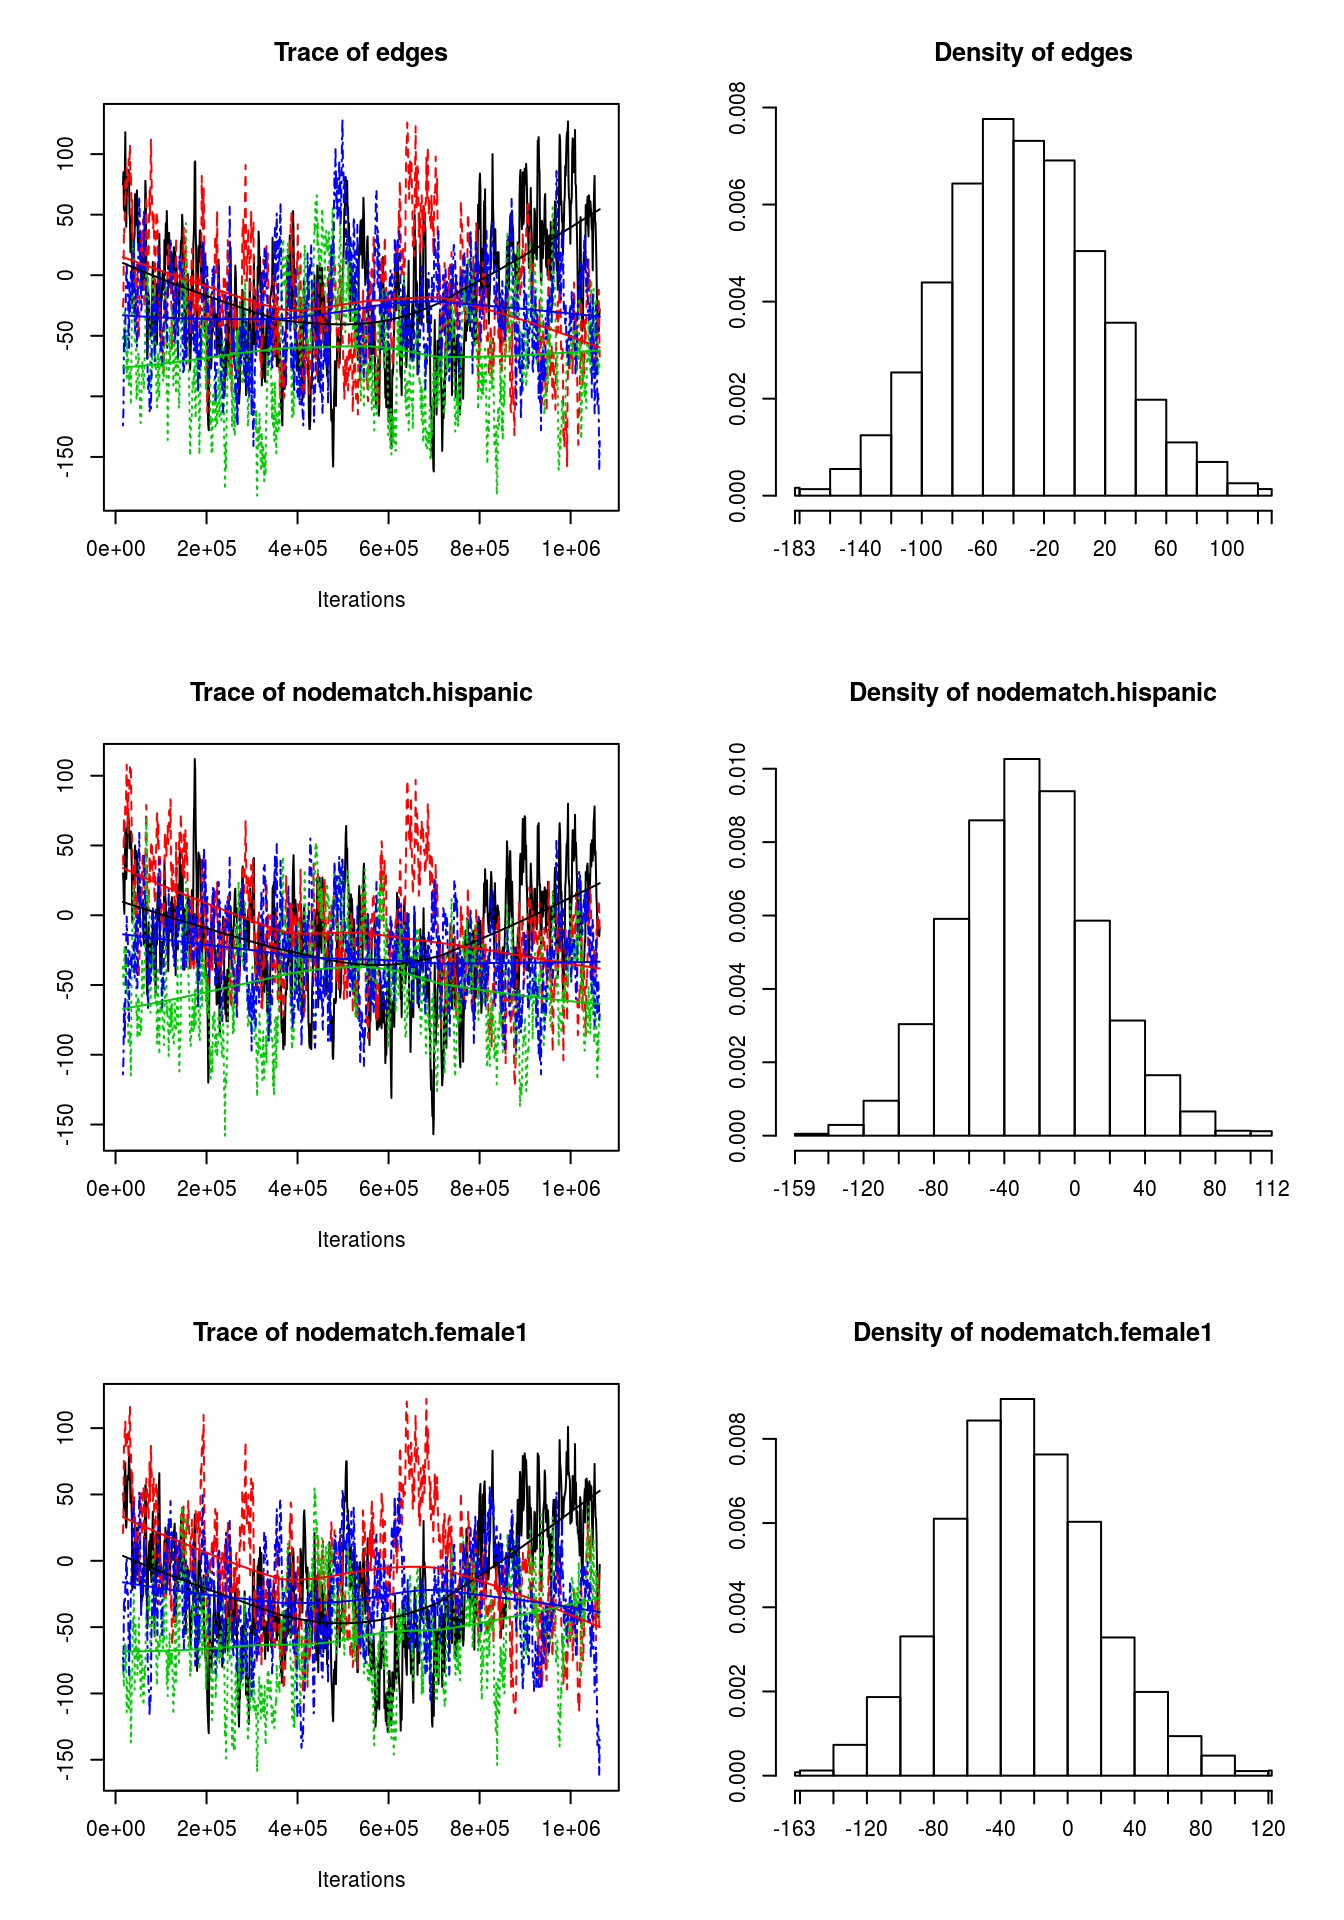
\includegraphics{04-ergms_files/figure-latex/coda-plots-1} 

}

\caption{Trace and posterior distribution of sampled network statistics.}\label{fig:coda-plots-1}
\end{figure}
\begin{figure}[!h]

{\centering 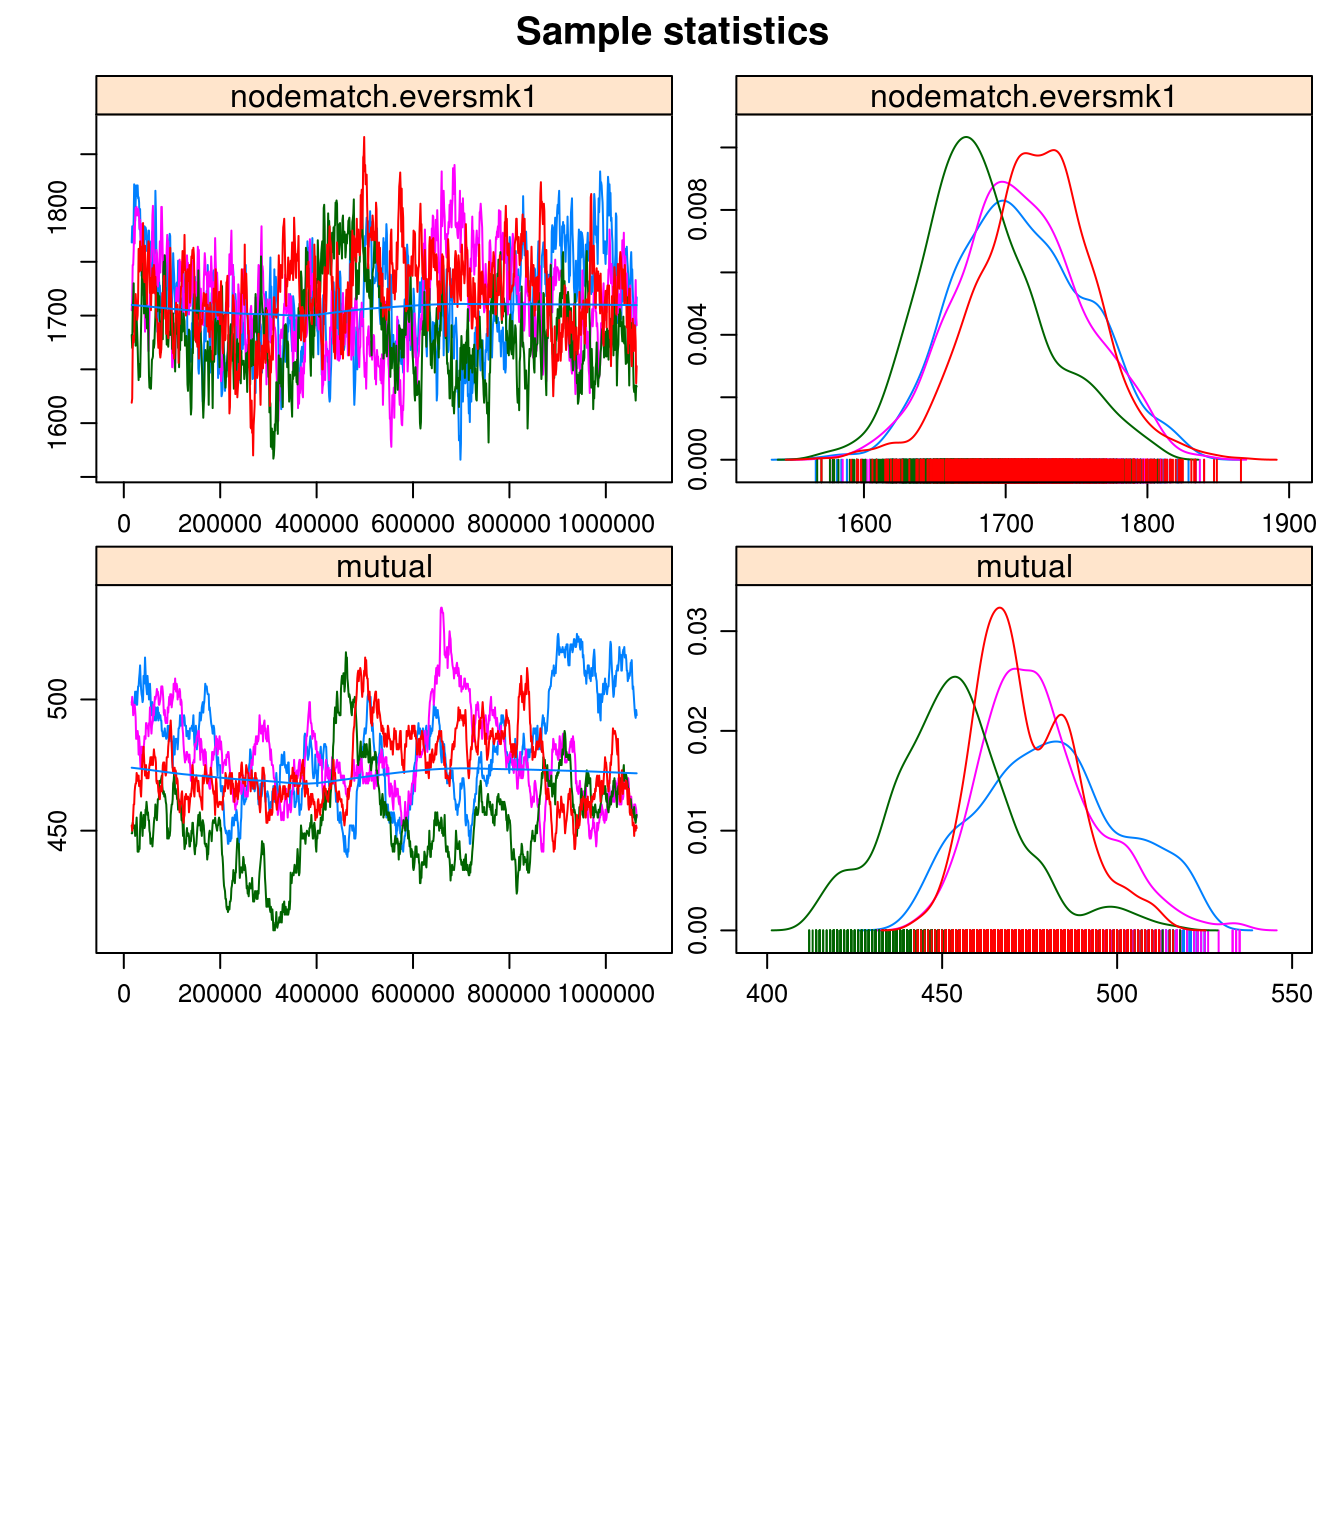
\includegraphics{04-ergms_files/figure-latex/coda-plots-2} 

}

\caption{Trace and posterior distribution of sampled network statistics (cont'd).}\label{fig:coda-plots-2}
\end{figure}

If we called the function \texttt{mcmc.diagnostics} this message appears at the end:

\begin{quote}
MCMC diagnostics shown here are from the last round of simulation, prior to computation of final parameter estimates. Because the final estimates are refinements of those used for this simulation run, these diagnostics may understate model performance. To directly assess the performance of the final model on in-model statistics, please use the GOF command: gof(ergmFitObject, GOF=\textasciitilde model).

---\texttt{mcmc.diagnostics(ans0)}
\end{quote}

Not that bad (although the \texttt{mutual} term could do better)!\footnote{The statnet wiki website as a very nice example of (very) bad and good mcmc diagnostics plots \href{https://statnet.org/trac/raw-attachment/wiki/Resources/ergm.fit.diagnostics.pdf}{here}.} First, observe that in the plot we see 4 different lines, why is that? Well, since we were running in parallel using 4 cores the algorithm actually ran 4 different chains of the MCMC algorithm. An eyeball test is to see if all the chains moved at about the same place, if we have that we can start thinking about model convergence from the mcmc perspective.

Once we are sure to have reach convergence on the MCMC algorithm, we can start thinking about how well does our model predicts the observed network's proterties. Besides of the statistics that define our ERGM, the \texttt{gof} function's default behavior show GOF for:

\begin{enumerate}
\def\labelenumi{\alph{enumi}.}
\tightlist
\item
  In degree distribution,
\item
  Out degree distribution,
\item
  Edge-wise shared partners, and
\item
  Geodesics
\end{enumerate}

Let's take a look at it

\begin{Shaded}
\begin{Highlighting}[]
\CommentTok{\# Computing and printing GOF estatistics}
\NormalTok{ans\_gof }\OtherTok{\textless{}{-}} \FunctionTok{gof}\NormalTok{(ans0)}
\NormalTok{ans\_gof}
\end{Highlighting}
\end{Shaded}

\begin{verbatim}
## 
## Goodness-of-fit for in-degree 
## 
##    obs min  mean max MC p-value
## 0   13   0  1.89   8       0.00
## 1   34   3  9.04  18       0.00
## 2   37  11 23.63  33       0.00
## 3   48  28 41.83  59       0.44
## 4   37  41 56.87  75       0.00
## 5   47  44 64.71  84       0.04
## 6   42  39 63.33  85       0.02
## 7   39  42 53.78  74       0.00
## 8   35  25 40.58  60       0.50
## 9   21  14 26.19  43       0.38
## 10  12   9 17.37  26       0.16
## 11  19   2  9.53  17       0.00
## 12   4   0  4.93  11       0.90
## 13   7   0  2.35   7       0.04
## 14   6   0  1.27   5       0.00
## 15   3   0  0.44   3       0.02
## 16   4   0  0.21   2       0.00
## 17   3   0  0.05   1       0.00
## 18   3   0  0.00   0       0.00
## 19   2   0  0.00   0       0.00
## 20   1   0  0.00   0       0.00
## 22   1   0  0.00   0       0.00
## 
## Goodness-of-fit for out-degree 
## 
##    obs min  mean max MC p-value
## 0    4   0  1.85   5       0.20
## 1   28   3  8.99  15       0.00
## 2   45  12 23.25  35       0.00
## 3   50  24 40.87  52       0.06
## 4   54  42 57.89  76       0.68
## 5   62  49 66.04  85       0.70
## 6   40  41 62.23  79       0.00
## 7   28  37 54.08  70       0.00
## 8   13  29 40.05  52       0.00
## 9   16  17 27.65  41       0.00
## 10  20   8 16.72  30       0.46
## 11   8   2  9.30  19       0.76
## 12  11   1  4.98  11       0.04
## 13  13   0  2.38   7       0.00
## 14   6   0  0.97   4       0.00
## 15   6   0  0.50   3       0.00
## 16   7   0  0.17   1       0.00
## 17   4   0  0.06   1       0.00
## 18   3   0  0.01   1       0.00
## 19   0   0  0.01   1       1.00
## 
## Goodness-of-fit for edgewise shared partner 
## 
##       obs  min    mean  max MC p-value
## esp0 1032 2012 2210.11 2303          0
## esp1  755  156  222.10  441          0
## esp2  352    4   13.42   93          0
## esp3  202    0    0.77   19          0
## esp4   79    0    0.04    3          0
## esp5   36    0    0.00    0          0
## esp6   14    0    0.00    0          0
## esp7    4    0    0.00    0          0
## esp8    1    0    0.00    0          0
## 
## Goodness-of-fit for minimum geodesic distance 
## 
##       obs   min     mean   max MC p-value
## 1    2475  2301  2446.44  2568       0.56
## 2   10672 12062 13688.54 14617       0.00
## 3   31134 48722 55636.04 60092       0.00
## 4   50673 77284 79447.41 81661       0.00
## 5   42563 14452 20165.40 26886       0.00
## 6   18719   325  1274.88  2453       0.00
## 7    4808     1    51.78   361       0.00
## 8     822     0     2.13   102       0.00
## 9     100     0     0.06     4       0.00
## 10      7     0     0.01     1       0.00
## Inf 12333     0  1593.31  4558       0.00
## 
## Goodness-of-fit for model statistics 
## 
##                     obs  min    mean  max MC p-value
## edges              2475 2301 2446.44 2568       0.56
## nodematch.hispanic 1615 1499 1578.58 1662       0.32
## nodematch.female1  1814 1690 1791.16 1883       0.54
## nodematch.eversmk1 1738 1595 1716.19 1834       0.56
## mutual              486  436  475.48  504       0.50
\end{verbatim}

\begin{Shaded}
\begin{Highlighting}[]
\CommentTok{\# Plotting GOF statistics}
\FunctionTok{plot}\NormalTok{(ans\_gof)}
\end{Highlighting}
\end{Shaded}

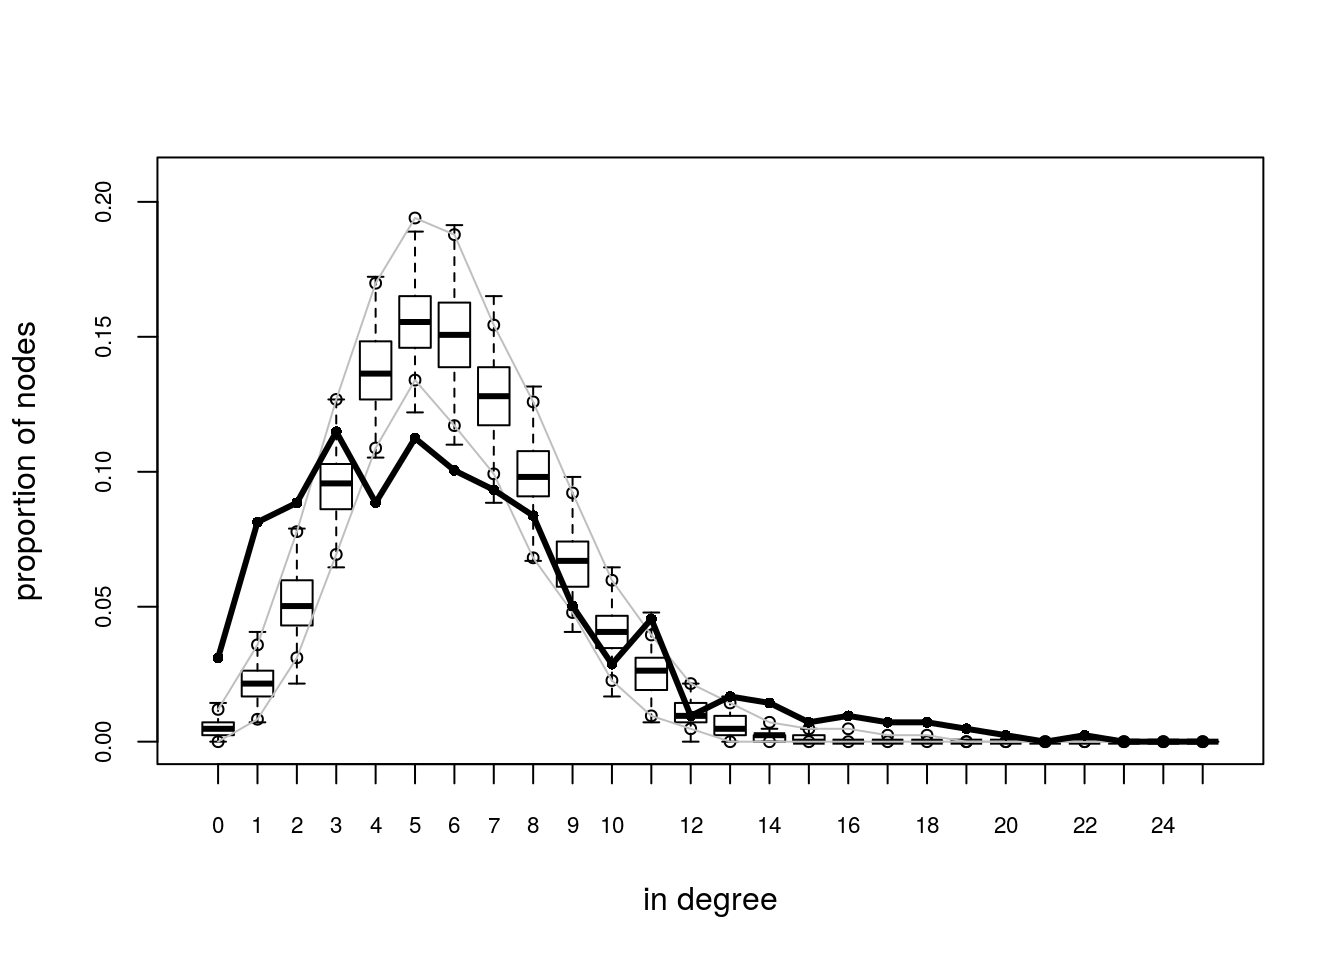
\includegraphics{04-ergms_files/figure-latex/checking-gof-1.pdf} 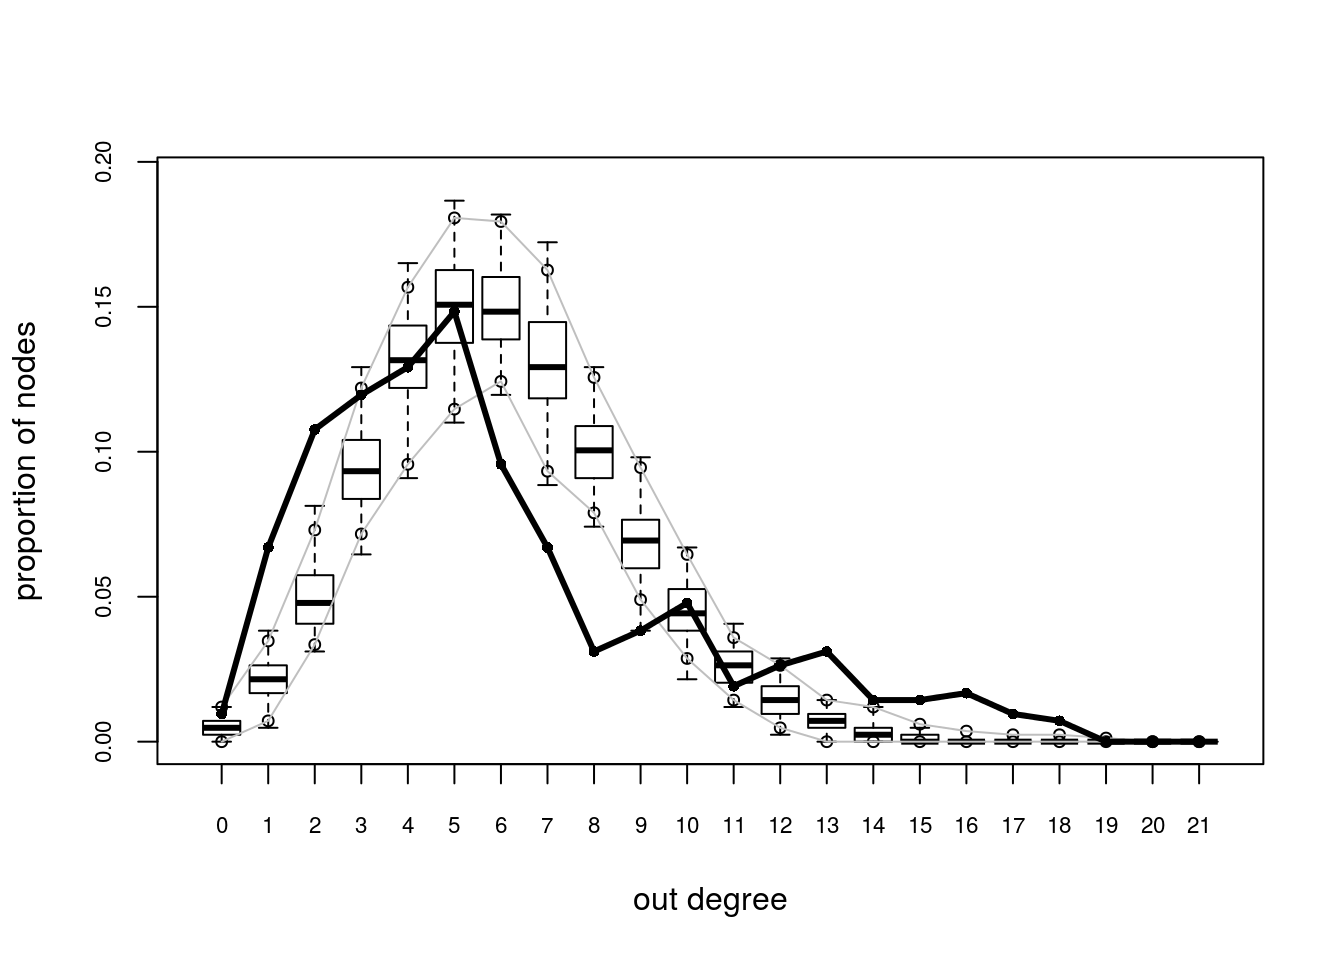
\includegraphics{04-ergms_files/figure-latex/checking-gof-2.pdf} 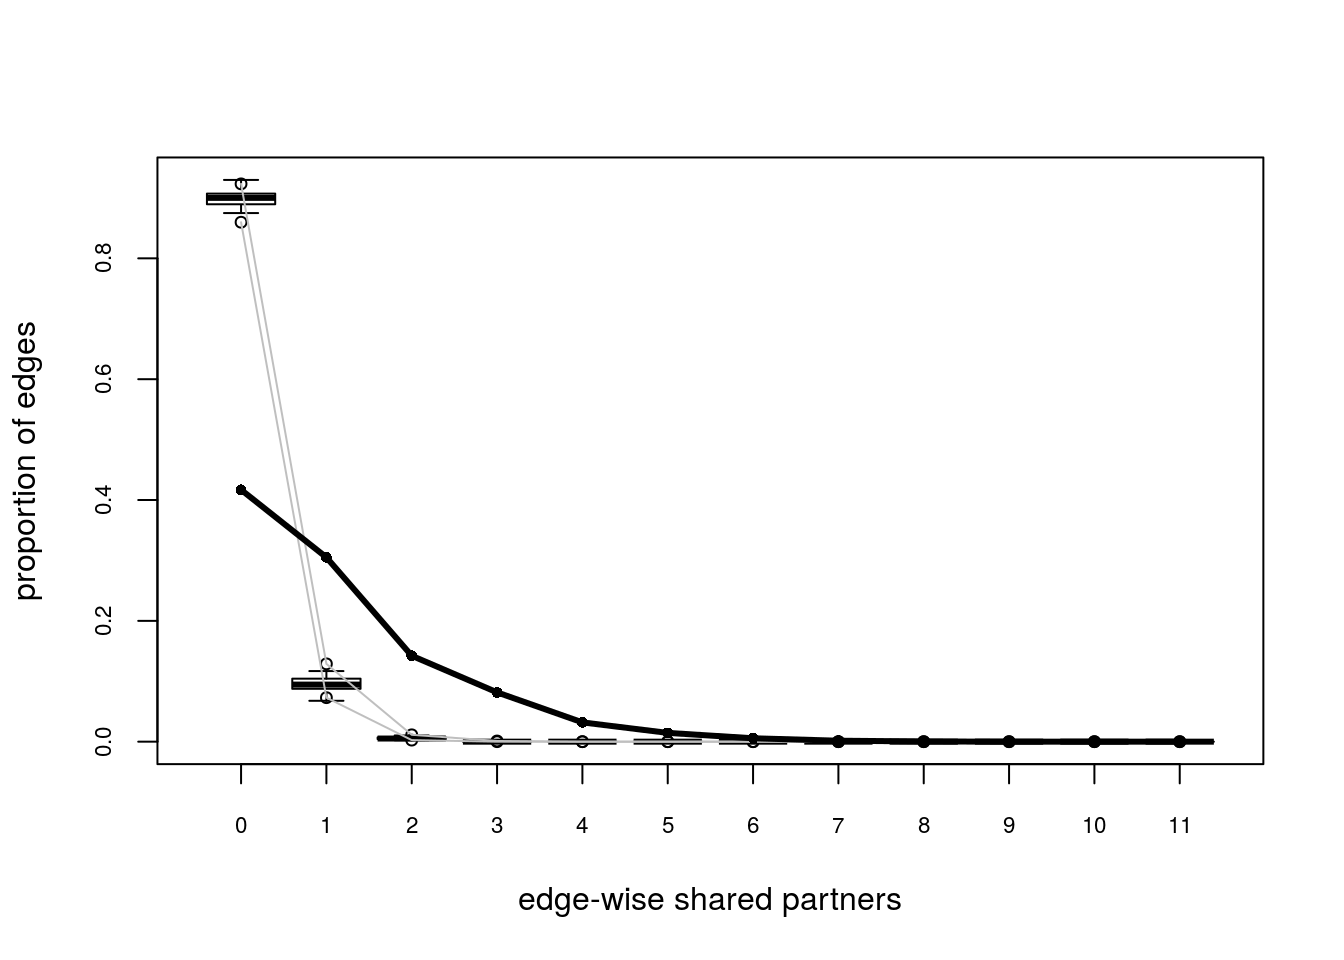
\includegraphics{04-ergms_files/figure-latex/checking-gof-3.pdf} 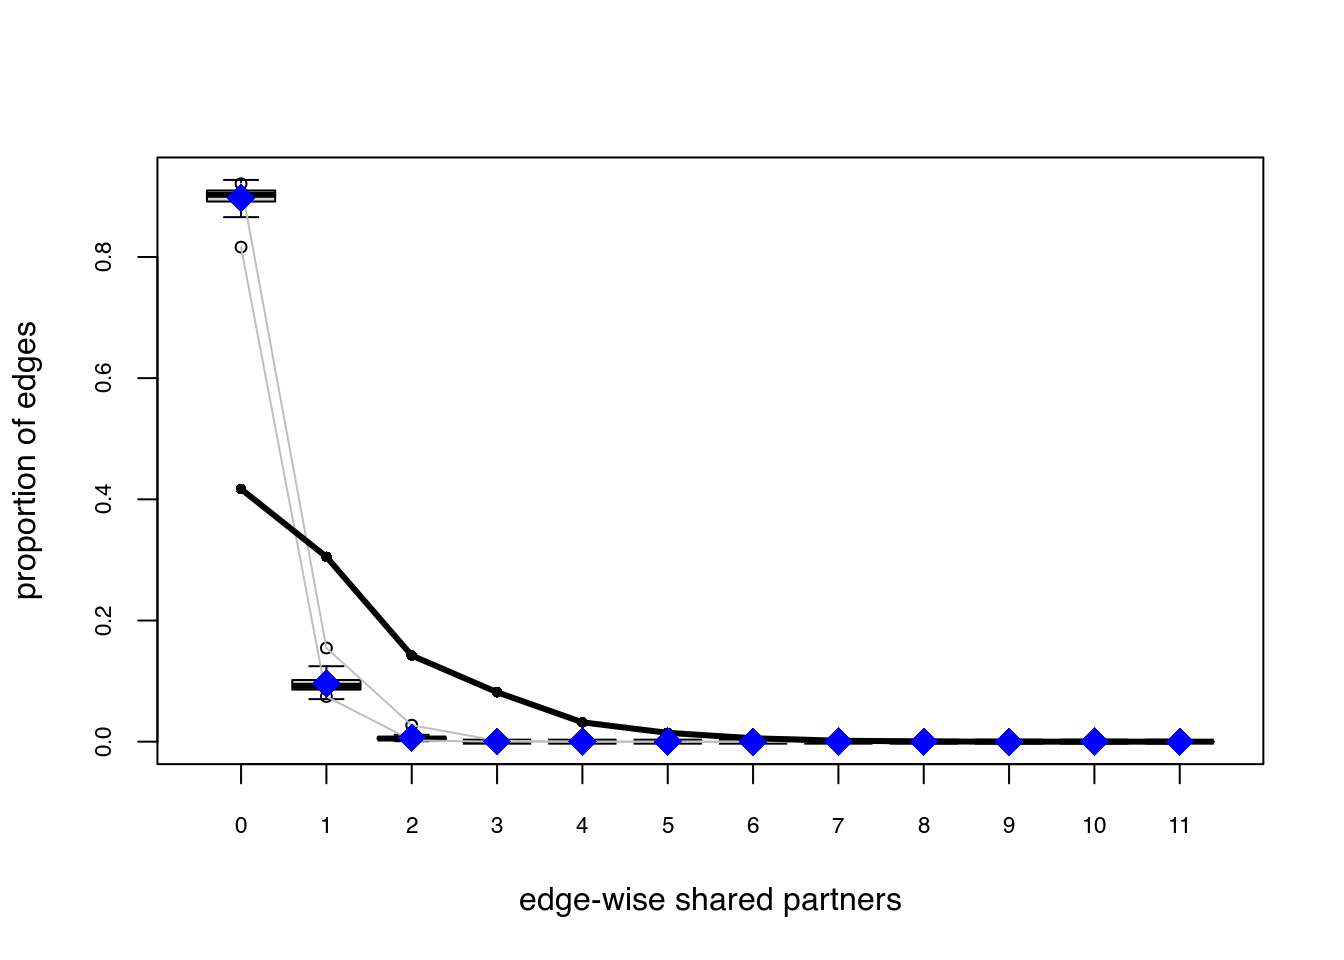
\includegraphics{04-ergms_files/figure-latex/checking-gof-4.pdf} 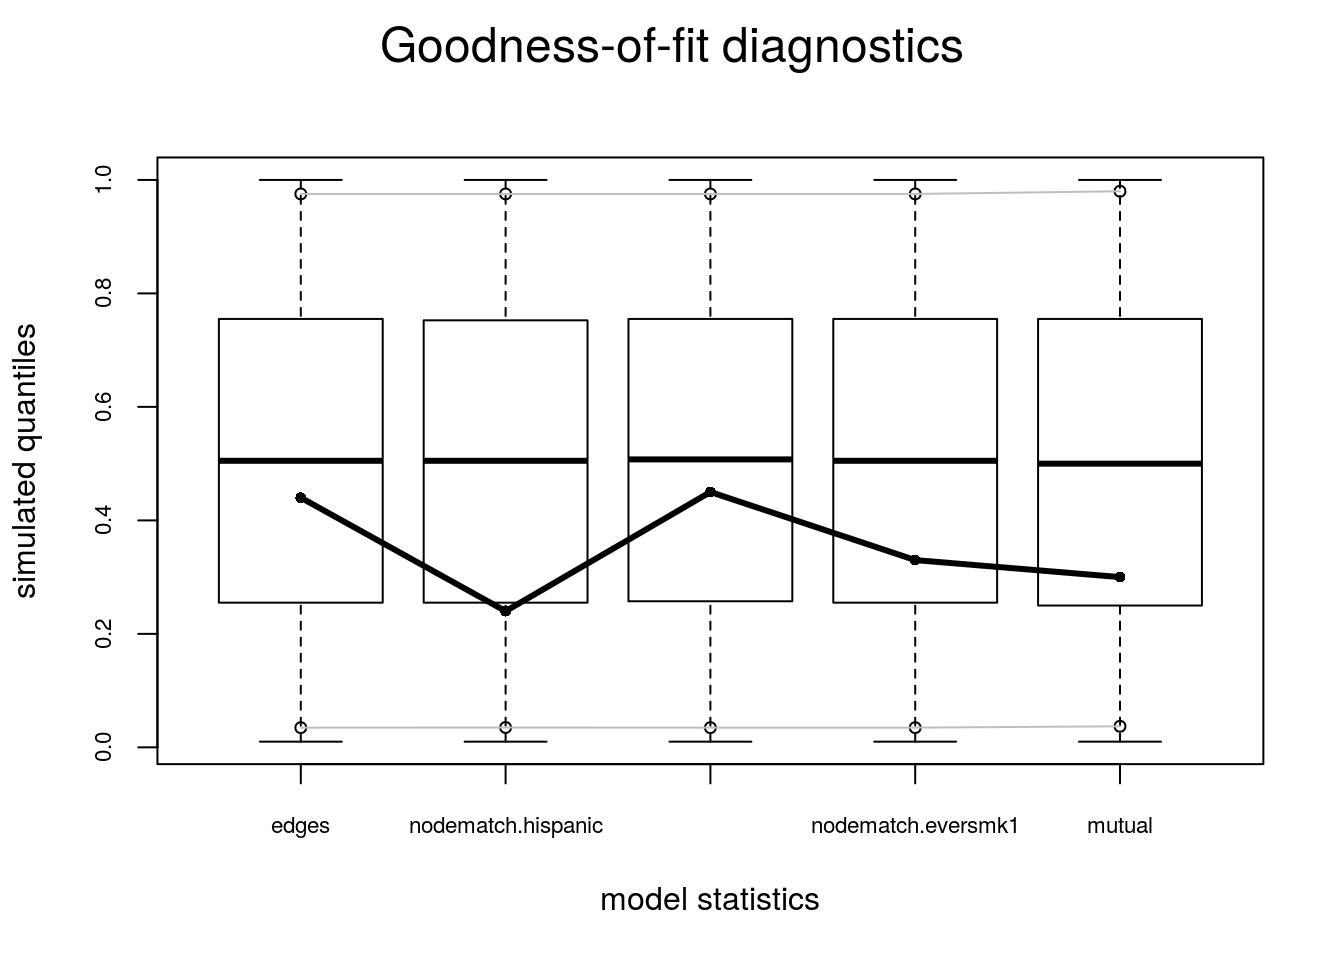
\includegraphics{04-ergms_files/figure-latex/checking-gof-5.pdf}

Try the following configuration instead

\begin{Shaded}
\begin{Highlighting}[]
\NormalTok{ans0\_bis }\OtherTok{\textless{}{-}} \FunctionTok{ergm}\NormalTok{(}
\NormalTok{  network\_111 }\SpecialCharTok{\textasciitilde{}}
\NormalTok{    edges }\SpecialCharTok{+}
    \FunctionTok{nodematch}\NormalTok{(}\StringTok{"hispanic"}\NormalTok{) }\SpecialCharTok{+}
    \FunctionTok{nodematch}\NormalTok{(}\StringTok{"female1"}\NormalTok{) }\SpecialCharTok{+}
\NormalTok{    mutual }\SpecialCharTok{+} 
    \FunctionTok{esp}\NormalTok{(}\DecValTok{0}\SpecialCharTok{:}\DecValTok{3}\NormalTok{) }\SpecialCharTok{+} 
    \FunctionTok{idegree}\NormalTok{(}\DecValTok{0}\SpecialCharTok{:}\DecValTok{10}\NormalTok{)}
\NormalTok{    ,}
  \AttributeTok{constraints =} \SpecialCharTok{\textasciitilde{}}\FunctionTok{bd}\NormalTok{(}\AttributeTok{maxout =} \DecValTok{19}\NormalTok{),}
  \AttributeTok{control =} \FunctionTok{control.ergm}\NormalTok{(}
    \AttributeTok{seed        =} \DecValTok{1}\NormalTok{,}
    \AttributeTok{MCMLE.maxit =} \DecValTok{15}\NormalTok{,}
    \AttributeTok{parallel    =} \DecValTok{4}\NormalTok{,}
    \AttributeTok{CD.maxit    =} \DecValTok{15}\NormalTok{,}
    \AttributeTok{MCMC.samplesize =} \DecValTok{2048}\SpecialCharTok{*}\DecValTok{4}\NormalTok{,}
    \AttributeTok{MCMC.burnin =} \DecValTok{30000}\NormalTok{,}
    \AttributeTok{MCMC.interval =} \DecValTok{2048}\SpecialCharTok{*}\DecValTok{4}
\NormalTok{    )}
\NormalTok{  )}
\end{Highlighting}
\end{Shaded}

Increase the sample size so the curves are more smooth, longer intervals (thinning) so we reduce the autocorrelation, larger burin. All this together to improve the Gelman test statistic. We also added idegree from 0 to 10, and esp from 0 to 3 to explicitly match those statistics in our model.

\begin{Shaded}
\begin{Highlighting}[]
\NormalTok{knitr}\SpecialCharTok{::}\FunctionTok{include\_graphics}\NormalTok{(}\StringTok{"awful{-}chains.png"}\NormalTok{)}
\end{Highlighting}
\end{Shaded}

\begin{figure}[!h]
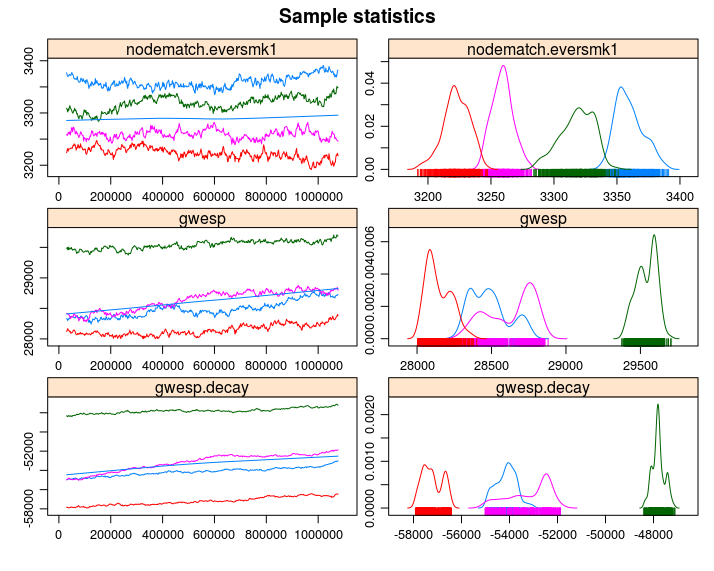
\includegraphics[width=9.92in]{awful-chains} \caption{An example of a terrible ERGM (no convergence at all). Also, a good example of why running multiple chains can be useful}\label{fig:badconvergence}
\end{figure}

\hypertarget{more-on-mcmc-convergence}{%
\section{More on MCMC convergence}\label{more-on-mcmc-convergence}}

For more on this issue, I recommend reviewing \href{http://www.mcmchandbook.net/HandbookChapter1.pdf}{chapter 1} and \href{http://www.mcmchandbook.net/HandbookChapter6.pdf}{chapter 6} from the Handbook of MCMC (\protect\hyperlink{ref-brooks2011}{Brooks et al. 2011}). Both chapters are free to download from the \href{http://www.mcmchandbook.net/HandbookSampleChapters.html}{book's website}.

For GOF take a look at section 6 of \href{https://statnet.csde.washington.edu/trac/raw-attachment/wiki/Sunbelt2016/ergm_tutorial.html}{ERGM 2016 Sunbelt tutorial}, and for a more technical review you can take a look at (\protect\hyperlink{ref-HunterJASA2008}{David R. Hunter, Goodreau, and Handcock 2008}).

\hypertarget{separable-temporal-exponential-family-random-graph-models}{%
\chapter{(Separable) Temporal Exponential Family Random Graph Models}\label{separable-temporal-exponential-family-random-graph-models}}

This tutorial is great! \url{https://statnet.org/trac/raw-attachment/wiki/Sunbelt2016/tergm_tutorial.pdf}

\hypertarget{stochastic-actor-oriented-models}{%
\chapter{Stochastic Actor Oriented Models}\label{stochastic-actor-oriented-models}}

Stochastic Actor Oriented Models (SOAM), also known as Siena models were introduced by CITATION NEEDED.

As a difference from ERGMs, Siena models look at the data generating process from the individuals' point of view. Based on McFadden's ideas of probabilistic choice, the model is founded in the following equation

\[
U_i(x) - U_i(x') \sim \mbox{Extreame Value Distribution}
\]

In other words, individuals choose between states \(x\) and \(x'\) in a probabilistic way (with some noise),

\[
\frac{\mbox{exp}\left\{f_i^Z(\beta^z,x, z)\right\}}{\sum_{Z'\in\mathcal{C}}\mbox{exp}\left\{f_i^{Z}(\beta, x, z')\right\}}
\]

snijders\_(sociological methodology 2001)

\protect\hyperlink{ref-Ripley2011}{Ripley et al.} (\protect\hyperlink{ref-Ripley2011}{2011})

\hypertarget{hypothesis-testing-in-networks}{%
\chapter{Hypothesis testing in networks}\label{hypothesis-testing-in-networks}}

Overall, there are many ways in which we can see hypothesis testing within
the networks context:

\begin{enumerate}
\def\labelenumi{\arabic{enumi}.}
\item
  \textbf{Comparing two or more networks}, e.g., we want to see if the density of
  two networks are \emph{equal}.
\item
  \textbf{Prevalence of a motif/pattern}, e.g., check whether the observed number
  of transitive triads is different from that expected as of by chance.
\item
  \textbf{Multivariate using ERGMs}, e.g., jointly test whether homophily and
  two stars are the motifs that drive network structure.
\end{enumerate}

The latter we already review in the ERGM chapter. In this part, we will look
at types one and two; both using non-parametric methods.

\hypertarget{comparing-networks}{%
\section{Comparing networks}\label{comparing-networks}}

Imagine that we have two graphs, \((G_1,G_2) \in \mathcal{G}\), and we would like
to assess whether a given statistic \(s(\cdot)\), e.g., density, is equal in both of them.
Formally, we would like to asses whether \(H_0: s(G_1) - s(G_2) = k\) vs
\(H_a: s(G_1) - s(G_2) \neq k\).

As usual, the true distribution of \(s(\cdot)\) is unknown, thus, one approach that
we could use is a non-parametric bootstrap test.

\hypertarget{network-bootstrap}{%
\subsection{Network bootstrap}\label{network-bootstrap}}

The non parametric bootstrap and jackknife methods for social networks were
introduced by (\protect\hyperlink{ref-Snijders1999}{T. A. B. Snijders and Borgatti 1999}). The method itself is used to generate standard
errors for network level statistics. Both methods are implemented in the R
package \href{https://cran.r-project.org/package=netdiffuseR}{\texttt{netdiffuseR}}.

\hypertarget{when-the-statistic-is-normal}{%
\subsubsection{When the statistic is normal}\label{when-the-statistic-is-normal}}

When the we deal with things that are normally distributed, e.g., sample means
like density\footnote{Density is indeed a sample mean as we are, in principle
  computing the average of a sequence of Bernoulli variables. Formally:
  \(\mbox{density}(G) = \frac{1}{n(n-1)}\sum_{ij}A_{ij}\).},
we can make use of the Student's distribution for making inference. In particular,
we can use Bootstrap/Jackknife to approximate the standard errors of the statistic
for each network:

\begin{enumerate}
\def\labelenumi{\arabic{enumi}.}
\item
  Since \(s(G_i)\sim \mbox{N}(\mu_i,\sigma_i^2/m_i)\) for \(i\in\{1,2\}\), in the case
  of the density, \(m_i = n_i * (n_i - 1)\). The statistic is then:

  \[
  s(G_1) - s(G_0)\sim \mbox{N}(\mu_1-\mu_0, \sigma_1^2/n_1 + \sigma_1^2/n_2)
  \]

  Thus

  \[
  \frac{s(G_1) - s(G_0) - \mu_1 + \mu_2}{\sqrt{\sigma_1^2/{m_1} + \sigma_1^2/{m_2}}} \sim t_{m_1 + m_2 - 2}
  \]
  But, if we are testing \(H_0: \mu_1 - \mu_2 = k\), then, under the null

  \[
  \frac{s(G_1) - s(G_0) - k}{\sqrt{\sigma_1^2/{m_1} + \sigma_1^2/{m_2}}} \sim t_{m_1 + m_2 - 2}
  \]
  Where We now proceede to approximate the variances.
\item
  Using the \emph{plugin principle} (\protect\hyperlink{ref-Efron1994}{Efron and Tibshirani 1994}), we can approximate the variances
  using Bootstrap/Jackknife, i.e., compute \(\hat\sigma_1^2\approx\sigma_1^2/m_1\) and
  \(\hat\sigma_2^2\approx\sigma_2^2/m_2\). Using netdiffuseR

\begin{Shaded}
\begin{Highlighting}[]
\FunctionTok{library}\NormalTok{(netdiffuseR)}

\CommentTok{\# Obtain a 100 replicates}
\NormalTok{sg1 }\OtherTok{\textless{}{-}} \FunctionTok{bootnet}\NormalTok{(g1, }\ControlFlowTok{function}\NormalTok{(i) }\FunctionTok{sum}\NormalTok{(i)}\SpecialCharTok{/}\NormalTok{(}\FunctionTok{nnodes}\NormalTok{(i) }\SpecialCharTok{*}\NormalTok{ (}\FunctionTok{nnodes}\NormalTok{(i) }\SpecialCharTok{{-}} \DecValTok{1}\NormalTok{)), }\AttributeTok{R =} \DecValTok{100}\NormalTok{)}
\NormalTok{sg2 }\OtherTok{\textless{}{-}} \FunctionTok{bootnet}\NormalTok{(g2, }\ControlFlowTok{function}\NormalTok{(i) }\FunctionTok{sum}\NormalTok{(i)}\SpecialCharTok{/}\NormalTok{(}\FunctionTok{nnodes}\NormalTok{(i) }\SpecialCharTok{*}\NormalTok{ (}\FunctionTok{nnodes}\NormalTok{(i) }\SpecialCharTok{{-}} \DecValTok{1}\NormalTok{)), }\AttributeTok{R =} \DecValTok{100}\NormalTok{)}

\CommentTok{\# Retrieving the variances}
\NormalTok{hat\_sigma1 }\OtherTok{\textless{}{-}}\NormalTok{ sg1}\SpecialCharTok{$}\NormalTok{var\_t}
\NormalTok{hat\_sigma2 }\OtherTok{\textless{}{-}}\NormalTok{ sg2}\SpecialCharTok{$}\NormalTok{var\_t}

\CommentTok{\# And the actual values}
\NormalTok{sg1 }\OtherTok{\textless{}{-}}\NormalTok{ sg1}\SpecialCharTok{$}\NormalTok{t0}
\NormalTok{sg2 }\OtherTok{\textless{}{-}}\NormalTok{ sg2}\SpecialCharTok{$}\NormalTok{t0}
\end{Highlighting}
\end{Shaded}
\item
  With the approximates in hand, we can then use the the ``t-test table'' to
  retrieve the corresponding value, in R:

\begin{Shaded}
\begin{Highlighting}[]
\CommentTok{\# Building the statistic}
\NormalTok{tstat }\OtherTok{\textless{}{-}}\NormalTok{ (sg1 }\SpecialCharTok{{-}}\NormalTok{ sg2 }\SpecialCharTok{{-}}\NormalTok{ k)}\SpecialCharTok{/}\NormalTok{(}\FunctionTok{sqrt}\NormalTok{(hat\_sigma1 }\SpecialCharTok{+}\NormalTok{ hat\_sigma2))}

\CommentTok{\# Computing the pvalue}
\NormalTok{m1 }\OtherTok{\textless{}{-}} \FunctionTok{nnodes}\NormalTok{(g1)}\SpecialCharTok{*}\NormalTok{(}\FunctionTok{nnodes}\NormalTok{(g1) }\SpecialCharTok{{-}} \DecValTok{1}\NormalTok{)}
\NormalTok{m2 }\OtherTok{\textless{}{-}} \FunctionTok{nnodes}\NormalTok{(g2)}\SpecialCharTok{*}\NormalTok{(}\FunctionTok{nnodes}\NormalTok{(g2) }\SpecialCharTok{{-}} \DecValTok{1}\NormalTok{)}
\FunctionTok{pt}\NormalTok{(tstat, }\AttributeTok{df =}\NormalTok{ m1 }\SpecialCharTok{+}\NormalTok{ m2 }\SpecialCharTok{{-}} \DecValTok{2}\NormalTok{)}
\end{Highlighting}
\end{Shaded}
\end{enumerate}

\hypertarget{when-the-statistic-is-not-normal}{%
\subsubsection{When the statistic is NOT normal}\label{when-the-statistic-is-not-normal}}

In the case that the statistic is not normally distributed, we cannot use the
t-statistic any longer. Nevertheless, the Bootstrap can come to help. While
in general it is better to use distributions of pivot statistics (see (\protect\hyperlink{ref-Efron1994}{Efron and Tibshirani 1994})),
we can still leverage the power of this method to make inferences. For this
example, \(s(\cdot)\) will be the range of the threshold in a diffusion graph.

As before, imagine that we are dealing with an statistic \(s(\cdot)\) for two
different networks, and we would like to asses whether we can reject \(H_0\)
or \href{https://www.thoughtco.com/fail-to-reject-in-a-hypothesis-test-3126424}{fail to reject} it.
The procedure is very similar:

\begin{enumerate}
\def\labelenumi{\arabic{enumi}.}
\item
  One approach that we can test is whether \(k \in \mbox{ConfInt}(s(G_1) - s(G_2))\).
  Building confidence intervals with bootstrap could be more intuitive.
\item
  Like before, we use bootstrap to generate a distribution of \(s(G_1)\) and
  \(s(G_2)\), in R:

\begin{Shaded}
\begin{Highlighting}[]
\CommentTok{\# Obtain a 1000 replicates}
\NormalTok{sg1 }\OtherTok{\textless{}{-}} \FunctionTok{bootnet}\NormalTok{(g1, }\ControlFlowTok{function}\NormalTok{(i) }\FunctionTok{range}\NormalTok{(}\FunctionTok{threshold}\NormalTok{(i)), }\AttributeTok{R =} \DecValTok{1000}\NormalTok{)}
\NormalTok{sg2 }\OtherTok{\textless{}{-}} \FunctionTok{bootnet}\NormalTok{(g2, }\ControlFlowTok{function}\NormalTok{(i) }\FunctionTok{range}\NormalTok{(}\FunctionTok{threshold}\NormalTok{(i)), }\AttributeTok{R =} \DecValTok{1000}\NormalTok{)}

\CommentTok{\# Retrieving the distributions}
\NormalTok{sg1 }\OtherTok{\textless{}{-}}\NormalTok{ sg1}\SpecialCharTok{$}\NormalTok{boot}\SpecialCharTok{$}\NormalTok{t}
\NormalTok{sg2 }\OtherTok{\textless{}{-}}\NormalTok{ sg2}\SpecialCharTok{$}\NormalTok{boot}\SpecialCharTok{$}\NormalTok{t}

\CommentTok{\# Define the statistic}
\NormalTok{sdiff }\OtherTok{\textless{}{-}}\NormalTok{ sg1 }\SpecialCharTok{{-}}\NormalTok{ sg2}
\end{Highlighting}
\end{Shaded}
\item
  Once we have \texttt{sdiff}, we can proceed and compute the, for example, 95\%
  confidence interval, and evaluate whether \(k\) falls within. In R:

\begin{Shaded}
\begin{Highlighting}[]
\NormalTok{diff\_ci }\OtherTok{\textless{}{-}} \FunctionTok{quantile}\NormalTok{(sdiff, }\AttributeTok{probs =} \FunctionTok{c}\NormalTok{(}\FloatTok{0.025}\NormalTok{, .}\DecValTok{975}\NormalTok{))}
\end{Highlighting}
\end{Shaded}
\end{enumerate}

This corresponds to what Efron and Tibshirani call ``percentile interval.''
This is easy to compute, but a better approach is using the ``BCa'' method,
``Bias Corrected and Accelerated.'' (TBD)

\cleardoublepage

\hypertarget{appendix-appendix}{%
\appendix}


\hypertarget{datasets}{%
\chapter{Datasets}\label{datasets}}

\hypertarget{sns-data}{%
\section{SNS data}\label{sns-data}}

\hypertarget{about-the-data}{%
\subsection{About the data}\label{about-the-data}}

\begin{itemize}
\item
  This data is part of the NIH Challenge grant \# RC 1RC1AA019239 ``Social
  Networks and Networking That Puts Adolescents at High Risk.''
\item
  In general terms, the SNS's goal was(is) ``Understand the network effects on
  risk behaviors such as smoking initiation and substance use.''
\end{itemize}

\hypertarget{variables}{%
\subsection{Variables}\label{variables}}

The data has a \emph{wide} structure, which means that there is one row per individual,
and that dynamic attributes are represented as one column per time.

\begin{itemize}
\item
  \texttt{photoid} Photo id at the school level (can be repeated across schools).
\item
  \texttt{school} School id.
\item
  \texttt{hispanic} Indicator variable that equals 1 if the indivual ever reported
  himself as hispanic.
\item
  \texttt{female1}, \ldots, \texttt{female4} Indicator variable that equals 1 if the individual
  reported to be female at the particular wave.
\item
  \texttt{grades1},\ldots, \texttt{grades4} Academic grades by wave. Values from 1 to 5, with 5
  been the best.
\item
  \texttt{eversmk1}, \ldots, \texttt{eversmk4} Indicator variable of ever smoking by wave. A one
  indicated that the individual had smoked at the time of the survey.
\item
  \texttt{everdrk1}, \ldots, \texttt{everdrk4} Indicator variable of ever drinking by wave.
  A one indicated that the individual had drink at the time of the survey.
\item
  \texttt{home1}, \ldots, \texttt{home4} Factor variable for home status by wave. A one
  indicates home ownership, a 2 rent, and a 3 a ``I don't know.''
\end{itemize}

During the survey, participants were asked to name up to 19 of their school
friends:

\begin{itemize}
\item
  \texttt{sch\_friend11}, \ldots, \texttt{sch\_friend119} School friends nominations (19 in total)
  for wave 1. The codes are mapped to the variable \texttt{photoid}.
\item
  \texttt{sch\_friend21}, \ldots, \texttt{sch\_friend219} School friends nominations (19 in total)
  for wave 2. The codes are mapped to the variable \texttt{photoid}.
\item
  \texttt{sch\_friend31}, \ldots, \texttt{sch\_friend319} School friends nominations (19 in total)
  for wave 3. The codes are mapped to the variable \texttt{photoid}.
\item
  \texttt{sch\_friend41}, \ldots, \texttt{sch\_friend419} School friends nominations (19 in total)
  for wave 4. The codes are mapped to the variable \texttt{photoid}.
\end{itemize}

\bibliographystyle{apacite}

\hypertarget{references}{%
\chapter*{References}\label{references}}
\addcontentsline{toc}{chapter}{References}

\hypertarget{refs}{}
\begin{CSLReferences}{1}{0}
\leavevmode\hypertarget{ref-admiraal2006}{}%
Admiraal, Ryan, and Mark S Handcock. 2006. {``Sequential Importance Sampling for Bipartite Graphs with Applications to Likelihood-Based Inference.''} Department of Statistics, University of Washington.

\leavevmode\hypertarget{ref-R-magrittr}{}%
Bache, Stefan Milton, and Hadley Wickham. 2014. \emph{Magrittr: A Forward-Pipe Operator for r}. \url{https://CRAN.R-project.org/package=magrittr}.

\leavevmode\hypertarget{ref-R-intergraph}{}%
Bojanowski, Michal. 2015. \emph{Intergraph: Coercion Routines for Network Data Objects}. \url{http://mbojan.github.io/intergraph}.

\leavevmode\hypertarget{ref-brooks2011}{}%
Brooks, Steve, Andrew Gelman, Galin Jones, and Xiao-Li Meng. 2011. \emph{Handbook of Markov Chain Monte Carlo}. CRC press.

\leavevmode\hypertarget{ref-R-igraph}{}%
Csardi, Gabor, and Tamas Nepusz. 2006. {``The Igraph Software Package for Complex Network Research.''} \emph{InterJournal} Complex Systems: 1695. \url{http://igraph.org}.

\leavevmode\hypertarget{ref-Efron1994}{}%
Efron, Bradley, and Robert J Tibshirani. 1994. \emph{An Introduction to the Bootstrap}. CRC press.

\leavevmode\hypertarget{ref-Geyer1992}{}%
Geyer, Charles J., and Elizabeth A. Thompson. 1992. {``Constrained Monte Carlo Maximum Likelihood for Dependent Data.''} \emph{Journal of the Royal Statistical Society. Series B (Methodological)} 54 (3): 657--99. \url{http://www.jstor.org/stable/2345852}.

\leavevmode\hypertarget{ref-R-statnet}{}%
Handcock, Mark S., David R. Hunter, Carter T. Butts, Steven M. Goodreau, Pavel N. Krivitsky, Skye Bender-deMoll, and Martina Morris. 2016. \emph{Statnet: Software Tools for the Statistical Analysis of Network Data}. The Statnet Project (\url{http://www.statnet.org}). \href{https://CRAN.R-project.org/package=statnet}{CRAN.R-project.org/package=statnet}.

\leavevmode\hypertarget{ref-R-ergm}{}%
Handcock, Mark S., David R. Hunter, Carter T. Butts, Steven M. Goodreau, Pavel N. Krivitsky, and Martina Morris. 2017. \emph{Ergm: Fit, Simulate and Diagnose Exponential-Family Models for Networks}. The Statnet Project (\url{http://www.statnet.org}). \url{https://CRAN.R-project.org/package=ergm}.

\leavevmode\hypertarget{ref-Hunter2008}{}%
Hunter, David R., Mark S. Handcock, Carter T. Butts, Steven M. Goodreau, and Martina Morris. 2008. {``{ergm : A Package to Fit, Simulate and Diagnose Exponential-Family Models for Networks}.''} \emph{Journal of Statistical Software} 24 (3). \url{https://doi.org/10.18637/jss.v024.i03}.

\leavevmode\hypertarget{ref-HunterJASA2008}{}%
Hunter, David R, Steven M Goodreau, and Mark S Handcock. 2008. {``Goodness of Fit of Social Network Models.''} \emph{Journal of the American Statistical Association} 103 (481): 248--58. \url{https://doi.org/10.1198/016214507000000446}.

\leavevmode\hypertarget{ref-lazega2015}{}%
Lazega, Emmanuel, and Tom AB Snijders. 2015. \emph{Multilevel Network Analysis for the Social Sciences: Theory, Methods and Applications}. Vol. 12. Springer.

\leavevmode\hypertarget{ref-R-texreg}{}%
Leifeld, Philip. 2013. {``{texreg}: Conversion of Statistical Model Output in {R} to {LaTeX} and {HTML} Tables.''} \emph{Journal of Statistical Software} 55 (8): 1--24. \url{http://www.jstatsoft.org/v55/i08/}.

\leavevmode\hypertarget{ref-lusher2012}{}%
Lusher, Dean, Johan Koskinen, and Garry Robins. 2012. \emph{Exponential Random Graph Models for Social Networks: Theory, Methods, and Applications}. Cambridge University Press.

\leavevmode\hypertarget{ref-Matloff2011}{}%
Matloff, Norman. 2011. \emph{The Art of r Programming: A Tour of Statistical Software Design}. No Starch Press.

\leavevmode\hypertarget{ref-Morris2008}{}%
Morris, Martina, Mark Handcock, and David Hunter. 2008. {``Specification of Exponential-Family Random Graph Models: Terms and Computational Aspects.''} \emph{Journal of Statistical Software, Articles} 24 (4): 1--24. \url{https://doi.org/10.18637/jss.v024.i04}.

\leavevmode\hypertarget{ref-R-coda}{}%
Plummer, Martyn, Nicky Best, Kate Cowles, and Karen Vines. 2006. {``{CODA}: Convergence Diagnosis and Output Analysis for MCMC.''} \emph{R News} 6 (1): 7--11. \url{https://journal.r-project.org/archive/}.

\leavevmode\hypertarget{ref-R-foreign}{}%
R Core Team. 2017a. \emph{Foreign: Read Data Stored by 'Minitab', 's', 'SAS', 'SPSS', 'Stata', 'Systat', 'Weka', 'dBase', ...} \url{https://CRAN.R-project.org/package=foreign}.

\leavevmode\hypertarget{ref-R}{}%
---------. 2017b. \emph{R: A Language and Environment for Statistical Computing}. Vienna, Austria: R Foundation for Statistical Computing. \url{https://www.R-project.org/}.

\leavevmode\hypertarget{ref-Ripley2011}{}%
Ripley, Ruth M., Tom AB Snijders, Paulina Preciado, and Others. 2011. {``{Manual for RSIENA}.''} \emph{University of Oxford: Department of Statistics, Nuffield College}, no. 2007. \url{https://www.uni-due.de/hummell/sna/R/RSiena_Manual.pdf}.

\leavevmode\hypertarget{ref-R-latticeExtra}{}%
Sarkar, Deepayan, and Felix Andrews. 2016. \emph{latticeExtra: Extra Graphical Utilities Based on Lattice}. \url{https://CRAN.R-project.org/package=latticeExtra}.

\leavevmode\hypertarget{ref-Snijders1999}{}%
Snijders, Tom A B, and Stephen P Borgatti. 1999. {``{Non-Parametric Standard Errors and Tests for Network Statistics}.''} \emph{Connections} 22 (2): 1--10. \url{https://insna.org/PDF/Connections/v22/1999_I-2_61-70.pdf}.

\leavevmode\hypertarget{ref-Snijders2010}{}%
Snijders, Tom A B, Gerhard G. van de Bunt, and Christian E G Steglich. 2010. {``{Introduction to stochastic actor-based models for network dynamics}.''} \emph{Social Networks} 32 (1): 44--60. \url{https://doi.org/10.1016/j.socnet.2009.02.004}.

\leavevmode\hypertarget{ref-Snijders2002}{}%
Snijders, Tom AB. 2002. {``Markov Chain Monte Carlo Estimation of Exponential Random Graph Models.''} \emph{Journal of Social Structure} 3.

\leavevmode\hypertarget{ref-R-rex}{}%
Ushey, Kevin, Jim Hester, and Robert Krzyzanowski. 2017. \emph{Rex: Friendly Regular Expressions}. \url{https://CRAN.R-project.org/package=rex}.

\leavevmode\hypertarget{ref-Wang2009}{}%
Wang, Peng, Ken Sharpe, Garry L. Robins, and Philippa E. Pattison. 2009. {``Exponential Random Graph (p*) Models for Affiliation Networks.''} \emph{Social Networks} 31 (1): 12--25. https://doi.org/\url{https://doi.org/10.1016/j.socnet.2008.08.002}.

\leavevmode\hypertarget{ref-R-stringr}{}%
Wickham, Hadley. 2017. \emph{Stringr: Simple, Consistent Wrappers for Common String Operations}. \url{https://CRAN.R-project.org/package=stringr}.

\leavevmode\hypertarget{ref-R-readxl}{}%
Wickham, Hadley, and Jennifer Bryan. 2017. \emph{Readxl: Read Excel Files}. \url{https://CRAN.R-project.org/package=readxl}.

\leavevmode\hypertarget{ref-R-dplyr}{}%
Wickham, Hadley, Romain Francois, Lionel Henry, and Kirill Müller. 2017. \emph{Dplyr: A Grammar of Data Manipulation}. \url{https://CRAN.R-project.org/package=dplyr}.

\leavevmode\hypertarget{ref-R-tidyr}{}%
Wickham, Hadley, and Lionel Henry. 2017. \emph{Tidyr: Easily Tidy Data with 'Spread()' and 'Gather()' Functions}. \url{https://CRAN.R-project.org/package=tidyr}.

\leavevmode\hypertarget{ref-R-readr}{}%
Wickham, Hadley, Jim Hester, and Romain Francois. 2017. \emph{Readr: Read Rectangular Text Data}. \url{https://CRAN.R-project.org/package=readr}.

\end{CSLReferences}

\end{document}
